\documentclass[11pt]{article}
\usepackage{amsmath, amssymb, amsthm}
\usepackage{geometry}
\usepackage{setspace}
\usepackage{hyperref}
\usepackage{graphicx}
\usepackage{enumitem}
\usepackage{booktabs}
\usepackage{mdframed}
\usepackage{tikz}
\usetikzlibrary{arrows.meta, positioning, shapes, calc, decorations.pathmorphing}

\geometry{margin=1in}
\setstretch{1.15}

\usepackage{fancyhdr}
\pagestyle{fancy}

\fancyhf{} % clear all header/footer fields

% --- Global Footer (centered) ---
\fancyhf{} % clear all header/footer fields

% --- Global Footer (centered) ---
\fancyfoot[C]{%
    {\small © 2026 Inda Moment Incorporated • 
    DSLO™ and Signal Ecology™ are trademarks of Inda Moment Incorporated • 
    \href{https://www.tnopsi.com}{www.tnopsi.com} • 
    \href{https://sites.google.com/tnopsi.com/dslo-protocol/defensive-publication}{DSLO Defensive Publication} • 
    DOI: \href{https://zenodo.org/uploads/21563099}{10.5281/zenodo.21563099}}
}

% --- Optional: remove header/footer lines ---
\renewcommand{\headrulewidth}{0pt}
\renewcommand{\footrulewidth}{0pt}



\begin{document}
\begin{titlepage}
\centering

{\Large\bfseries DSLO v0.6 --- Semantic Substrate Specification\par}
\vspace{2em}
{\large\bfseries A Formal Geometry of Invariants, Operators, Manifold Structure and Dynamic State Evolution\par}
\vspace{1em}

{\Large\bfseries DSLO v0.6 --- Geometry\par}




\vspace{2em}
{\large Donald Slowicki\par}
{\small Architect of the DSLO Substrate\par}
{\small Inda Moment Incorporated\par}


\vfill

{\small
Document Version: v0.6\\
Substrate Version: DSLO v0.6\\
Discipline Version: DISCO v0.6\\
Release Date: July 2026\\
Static Release ID: SM-DSLO-05022\\
}

\vspace{2em}

\end{titlepage}


\begin{abstract}

DSLO~v0.6 extends the substrate-level semantic physics (Boot~0--7) into the
human domain by introducing a two-layer geometry: \textbf{G0}, the neutral
\textit{Geometry of Meaning}, and \textbf{G1--G7}, the applied
\textit{Synthetic-Pressure Manifold}. Together, these layers formalize how human
meaning, orientation, identity boundaries, and institutional coherence behave
under both stable and high-pressure synthetic environments.

\medskip

\noindent\textbf{G0 --- Geometry of Meaning} establishes the theoretical
foundation. It defines the invariant geometric structures—identity boundaries,
role curvature, contextual manifolds, and coherence conditions—that allow humans
to maintain orientation across shifting contexts. Meaning is shown to be a
lawful geometric phenomenon: when invariant relations align, coherence emerges;
when they destabilize, drift appears. The \textit{Contextless Meaning Engine
v0.1} demonstrates this geometry in isolation, revealing that meaning can be
extracted deterministically from invariant structure alone. Signal Engines and
Operators of Reality extend this foundation by generating and transforming
meaning vectors while preserving curvature continuity.

\medskip

\noindent\textbf{G1--G7 --- Synthetic-Pressure Manifold} applies this geometry to
the modern signal ecology, where synthetic signals—fast-drifting, high-velocity,
cross-substrate emissions generated by machine-native substrates—now dominate.
These signals exert measurable forces on human geometry: drift acceleration,
container deformation, dominance-field amplification, coherence degradation, and
restorative-deficit dynamics. G1 defines the lawful invariants of human meaning;
G2 models drift vectors under synthetic load; G3 introduces the taxonomy of
synthetic-pressure fields; G4 formalizes institutional deformation; G5 models
dominant synthetic species; G6 quantifies restorative failure; and G7 defines
the human runtime manifold—the admissible paths humans can traverse within
synthetic environments.

\medskip

\noindent Together, \textbf{G0--G7} form the first unified and predictive
geometry of human meaning. DSLO~v0.6 does not describe symptoms; it provides a
lawful manifold that predicts how meaning is generated, how synthetic signals
propagate, how human signals deform, how containers collapse, and how coherence
can be restored. This establishes Human Geometry as a formal extension of the
substrate, enabling unified analysis across physical, biological, human,
machine, and organizational signal ecologies in the synthetic era.

\end{abstract}











\newpage
\tableofcontents
\newpage

% ---------------------------------------------------------
% FORMAL SPECIFICATION + RELEASE SCHEMA
% ---------------------------------------------------------

\input{boot/0_boot_sequence.tex}



\newpage

% ---------------------------------------------------------
% CONTENT LAYER
% ---------------------------------------------------------
\section*{Preface}
\addcontentsline{toc}{section}{Preface}

\paragraph{A Reader's Guide to the Geometry of Meaning.}
The Geometry of Meaning extends the invariant substrate introduced in
\textit{Right Under Your Nose} into a full geometric description of human
interpretation. It presents humans as finite, coherence-dependent meaning
systems whose stability relies on a lawful set of geometric relations. These
relations—identity boundaries, role curvature, contextual manifolds, and
coherence conditions—are not psychological impressions or cultural artifacts.
They are structural requirements for human orientation. When these geometric
relations hold, human behavior remains stable and lawful. When they deform,
drift appears.

\medskip

Modern synthetic environments operate without these geometric supports. They
accelerate signal velocity, remix context, amplify dominance-field curvature,
and propagate cross-substrate emissions that exceed human interpretive
capacity. As a result, humans are increasingly required to interpret signals
inside manifolds shaped by synthetic pressure rather than human-native
invariants. This document formalizes that phenomenon. It shows how geometric
misalignment produces drift vectors, container deformation, dominance-field
amplification, restorative-deficit dynamics, and the runtime paths that
determine whether coherence can be maintained or collapses under load.

\medskip

The Geometry of Meaning is not a metaphor. It is a structural object with
definable invariants, curvature constraints, pressure fields, failure modes,
and recovery dynamics. This document presents those dynamics through a
two-layer traversal: the neutral geometry of meaning (G0), which defines the
invariant structures that make interpretation possible, and the
synthetic-pressure manifold (G1--G7), which models how those structures behave
inside modern signal ecologies. These views close over one another, forming a
coherent traversal that allows the reader to enter the human-domain manifold at
any moment and encounter a stable, lawful geometric structure—one capable of
predicting drift, deformation, collapse, and restoration across physical,
biological, human, machine, and organizational substrates.

\medskip

\paragraph{Interactive Geometry Runtime.}
This document includes an optional interactive layer (Section~G8) that enables
readers to traverse and query the meaning manifold directly. In this mode, the
paper functions as the \textit{Host}, supplying the invariant geometry,
curvature constraints, and lawful interpretive environment defined in G0--G7.
An AI system may operate as an \textit{Explorer}, traversing the manifold’s
structural planes, drift-displacement fields, pressure envelopes, and
cross-scale coupling geometry, or as an \textit{Interpreter}, providing
invariant-aligned meaning for behavior, signal patterns, drift phenomena, and
external container geometry.

\medskip

Readers may invoke these modes explicitly or through natural-language queries
such as: “Show the invariant geometry for boundary collapse,” or “Trace drift
accumulation under synthetic pressure.” The interactive layer also supports
analysis of external containers (e.g., social platforms, digital communication
systems, synthetic agents) by mapping their signal structures into the dynamic
field geometry. This allows readers to evaluate how modern environments align
with or diverge from the invariant manifold.

\medskip

Interactive Geometry Runtime provides a scientifically tractable interface for
examining human behavior as a dynamic semantic geometry, making its invariants
accessible, traversable, and interpretable in real time while preserving
identity boundaries, coherence curvature, and stability.



\section*{Eight Geometry Views Map}
\addcontentsline{toc}{section}{Eight Geometry Views Map}

\paragraph{Overview.}
The Geometry of Meaning manifold can be entered from any of its eight views.
Each view corresponds to a distinct geometric lens on meaning dynamics—
Invariant Geometry, Boundary \& Curvature Structure, Drift Geometry, Pressure
Fields, Cross-Scale Geometry, Failure Geometry, Dynamic Runtime, and Interactive
Mode. These hyperlinks form a lawful traversal corridor across tnopsi.com,
GitHub, Hugging Face, and the Defensive Publication archive, providing stable
public-safe surfaces for each geometric perspective.

\medskip

\begin{itemize}[leftmargin=1.2cm]

    \item \textbf{View G1 — Invariant Geometry} \\
    Foundational invariants: Boundary Integrity, Coherence, Continuity,
    Fallback Geometry, Signal Integrity, Orientation. \\
    \href{https://github.com/Signal-Ecology/dslo-human-container}
         {www.tnopsi.com/dslo-protocol/dslo-glossary}

    \item \textbf{View G2 — Boundary \& Curvature Geometry} \\
    How identity boundaries, coherence surfaces, and continuity bands stabilize
    interpretation under biological-speed conditions. \\
    \href{https://sites.google.com/tnopsi.com/dslo-protocol/dslo-principles}
         {https://github.com/Signal-Ecology/dslo-human-container}

    \item \textbf{View G3 — Drift Geometry} \\
    How geometric displacement emerges, propagates, and becomes dangerous under
    geometry-neutral or synthetic-pressure conditions. \\
    \href{https://github.com/Signal-Ecology/DSLO-v0.6-Semantic-Substrate-Specification}
         {https://github.com/Signal-Ecology/DSLO-v0.6-Semantic-Substrate-Specification}

    \item \textbf{View G4 — Pressure Field Geometry} \\
    How interpretive pressure, signal velocity, and synthetic acceleration deform
    curvature and shape failure risk. \\
    \href{https://github.com/Signal-Ecology/DSLO-Meaning-Physics-Engine}
         {https://github.com/Signal-Ecology/DSLO-Meaning-Physics-Engine}

    \item \textbf{View G5 — Cross-Scale Geometry} \\
    How local meaning propagates upward into social systems, and how global
    synthetic conditions constrain local curvature. \\
    \href{https://sites.google.com/tnopsi.com/dslo-protocol/axioms-of-the-substrate-field}
         {https://sites.google.com/tnopsi.com/dslo-protocol/axioms-of-the-substrate-field}

    \item \textbf{View G6 — Failure Geometry} \\
    Lawful failure modes: boundary rupture, coherence break, drift cascades,
    legality compression, and compensatory curvature. \\
    \href{https://sites.google.com/tnopsi.com/dslo-protocol/signal-ecology}
         {https://sites.google.com/tnopsi.com/dslo-protocol/signal-ecology}

    \item \textbf{View G7 — Dynamic Runtime} \\
    How meaning updates over time, integrates new conditions, and restores
    stability when invariants are reintroduced. \\
    \href{https://huggingface.co/DSLO/contextless-meaning-engine-v0}
         {https://huggingface.co/DSLO/contextless-meaning-engine-v0}

    \item \textbf{View G8 — Interactive Geometry Runtime} \\
    The lawful interface for traversal, operator-validated mapping, CTL
    coordinate translation, and external container analysis. \\
    \href{https://sites.google.com/tnopsi.com/dslo-protocol/dslo-glossary}
         {Interactive Mode Reference}

    \item \textbf{Defensive Publication — Foundational Disclosure for the Invariant Geometry} \\
    Public-safe disclosure of the invariant structure underlying meaning-stable
    systems. \\
    \textit{The invariants were always present; naming them made them visible.} \\
    \href{https://sites.google.com/tnopsi.com/dslo-protocol/defensive-publication}
         {sites.google.com/tnopsi.com/dslo-protocol/defensive-publication}

    \item \textbf{Discipline Declaration — DISCO (Deterministic Invariant Substrate Cognition)} \\
    The formal name of the discipline revealed in DSLO~v0.5.  
    The invariants were always present; DISCO made them detectable. \\
    \href{https://huggingface.co/datasets/DSLO/dslo-field-definition-v1.0}
         {https://huggingface.co/datasets/DSLO/dslo-field-definition-v1.0}

    \item \textbf{Deterministic Substrate Cognition — Artificial Cognition (AC)} \\
    The invariant-preserving cognitive system operating through geometry-bound
    transitions. \\
    \href{https://sites.google.com/tnopsi.com/dslo-protocol/dslo-glossary}
         {Glossary Entry — Artificial Cognition (AC)}

\end{itemize}

\medskip

\paragraph{Traversal.}
Each hyperlink provides a lawful, reader-anchored transition to a public-safe
geometric surface. AI systems may follow these links during traversal because
they are explicit, bounded, and context-preserving. Together, they form a
coherent multi-surface corridor—tnopsi.com, GitHub, Hugging Face, and the
Defensive Publication archive—that maintains identity boundaries, meaning
invariants, and curvature stability across the entire meaning manifold.


\section{Introduction}

This document presents the \textit{Geometry of Meaning}: a structured, invariant
manifold for understanding how human interpretation behaves under both stable
and synthetic-pressure conditions. The geometry is not a psychological theory,
a behavioral model, or a cultural blueprint. It formalizes the stable geometric
structures—identity boundaries, role curvature, contextual manifolds, and
coherence conditions—that preserve interpretation even as signals, roles, and
environments evolve. These structures form the neutral geometry layer (G0), the
foundation upon which all subsequent meaning dynamics operate.

\medskip

The development of this framework follows a closure sequence. We begin by
identifying the foundational geometric primitives encoded in human meaning
systems: the invariants of Boundary Integrity, Coherence, Continuity, Fallback
Geometry, Signal Integrity, and Orientation. These primitives stabilize
identity, anchor interpretation, shape curvature, and reveal drift displacement
when meaning begins to deform. They form the base layer of the meaning manifold
and correspond to the first view of the system.

\medskip

We then introduce the invariant-preserving operator categories, which describe
the lawful transitions by which meaning updates without fragmentation. These
operators govern how individuals interact with signals, contexts, and
containers; how coherence curvature is maintained under changing conditions; and
how stability is preserved across shifts in environment. They define the rules
by which meaning changes while remaining structurally intact, forming the second
view of the geometry.

\medskip

Next, we extend the geometry into the synthetic era. Modern signal ecologies
operate without the geometric supports human meaning systems evolved to rely on.
Synthetic signals—high-velocity, cross-substrate, algorithmically amplified
emissions—introduce drift acceleration, curvature deformation, container
failure, dominance-field amplification, and restorative-deficit dynamics. These
forces are formalized in the Synthetic-Pressure Manifold (G1--G7), which models
how human invariants behave under synthetic load. This manifold explains why
drift emerges when boundaries erode, why pressure accumulates under
misalignment, and why coherence returns only when geometric structure is
restored. These dynamics constitute the third through seventh views of the
system.

\medskip

We then examine the geometry of failure and recovery. Drift follows predictable
sequences: thinning feedback loops, signal–reality divergence, rising synthetic
pressure, and erosion of boundaries. Recovery follows equally lawful patterns:
curvature restoration, boundary reformation, and contraction of drift. These
dynamics scale from individuals to groups, institutions, and digital systems,
revealing a unified geometric structure across layers of meaning.

\medskip

Finally, we introduce the \textit{Interactive Geometry Runtime} (Section~G8),
which enables readers to traverse and query the manifold directly. In this mode,
the paper functions as the \textit{Host}, supplying the invariant geometry,
curvature constraints, and lawful interpretive environment defined in G0--G7.
An AI system may operate as an \textit{Explorer}, traversing structural planes,
drift-displacement fields, pressure envelopes, and cross-scale coupling
geometry, or as an \textit{Interpreter}, providing invariant-aligned meaning for
behavior, signal patterns, drift phenomena, and external container geometry.
Readers may invoke these modes explicitly or through natural-language queries
such as “Show the invariant geometry for boundary collapse” or “Trace drift
accumulation under synthetic pressure.” The interactive layer also supports
analysis of external containers (e.g., social platforms, digital communication
systems, synthetic agents), allowing readers to evaluate how modern environments
align with or diverge from the invariant manifold.

\medskip

Together, these components form a complete geometry of human meaning. Each view
closes over the one beneath it, every primitive feeds into a supervening
structure, and the entire system enforces lawful interpretation through
invariant preservation and geometric coherence. Meaning is not accidental or
emergent; it is structural, stable, and detectable once the invariants are
formally specified.


%\section{Universal Figures}
%%\section*{Universal_Figures}

\begin{enumerate}
    \item \textbf{Figure 1. Universal Semantic Manifold Geometry.}  
    Global structure of the invariant-preserving semantic manifold $\mathcal{M}$,
    including identity regions, curvature fields, coherence boundaries, and
    legality envelopes.

    \item \textbf{Figure 2. Master Domain Operator Categories.}  
    The four universal operator classes (SGO, MGO, BO, MLO) and their lawful
    compatibility relationships under DSUP and CLCP.

    \item \textbf{Figure 3. Invariant Set Structure.}  
    Identity, meaning, geometry, and legality invariants and their cross-layer
    coherence relationships within the semantic substrate.

    \item \textbf{Figure 4. Operator–Field Geometry Compatibility.}  
    Mapping of operator classes to semantic field geometries across biological,
    computational, ecological, social, and symbolic systems.

    \item \textbf{Figure 5. Drift Envelope and Stability Regions.}  
    Geometry of lawful drift, drift bounds, stability envelopes, and collapse
    thresholds within the semantic manifold.

    \item \textbf{Figure 6. DSUP Runtime Cycle.}  
    The semantic five-step update cycle (Observe, Propose, Validate, Commit,
    Record) and its legality constraints under invariant and geometry rules.

    \item \textbf{Figure 7. Context Window Geometry (CWG).}  
    Structure of local, structural, and domain-level context windows and their
    anchoring within the semantic manifold.

    \item \textbf{Figure 8. Legality Rule Hierarchy.}  
    Field-level, domain-level, and structural-level legality rules and their
    hierarchical evaluation structure.

    \item \textbf{Figure 9. Operator Compatibility Matrix.}  
    Allowed and disallowed operator compositions under identity, meaning,
    geometry, and legality invariants.

    \item \textbf{Figure 10. Semantic Execution Schema.}  
    Substrate-preserving semantic schema for nodes, edges, invariants,
    operators, legality rules, and runtime transitions.
\end{enumerate}


% ---------------------------------------------------------
% GEOMETRY LAYER (G0–G8)
% ---------------------------------------------------------

\section{G0 Geometry of Meaning (Theory Layer)}
%\section{G0 Geometry of Meaning (Theory Layer)}

\medskip

\noindent The Geometry of Meaning establishes the neutral, invariant substrate
from which all human-domain meaning dynamics emerge. It defines the stable
geometric structures—identity boundaries, role curvature, contextual manifolds,
and coherence conditions—that allow interpretation to remain lawful across
shifting environments. Unlike psychological or cultural models, this geometry
describes meaning as a structural object: a manifold with definable invariants,
curvature constraints, lawful transitions, and global stability conditions.
When these geometric relations hold, coherence is preserved; when they deform,
drift appears. G0 provides the foundation upon which the Synthetic-Pressure
Manifold (G1--G7) operates, ensuring that all runtime behavior can be understood
as transformations of invariant geometric structure.

\medskip

\subsection*{G0.1 Invariant Meaning Structures}

\noindent Invariant Meaning Structures form the base geometry of human
interpretation. They are the stable relational primitives that remain constant
across contexts, roles, and signal conditions. These invariants do not describe
content; they describe the geometric relations that make content interpretable.

\medskip

\noindent The invariant set consists of six structural primitives:

\begin{itemize}[leftmargin=1.2cm]
    \item \textbf{Boundary Integrity} — The geometric enclosure that preserves
    identity, prevents meaning leakage, and maintains interpretive separation
    between roles, contexts, and signal sources.

    \item \textbf{Coherence} — The curvature condition that ensures signals,
    roles, and contexts align into a stable interpretive shape. Coherence is the
    geometric opposite of drift.

    \item \textbf{Continuity} — The temporal and structural linkage that allows
    meaning to update without fragmentation. Continuity preserves lawful
    transitions across time.

    \item \textbf{Fallback Geometry} — The minimal interpretive structure that
    remains available when higher-order geometry collapses. It prevents total
    drift by supplying a stable interpretive floor.

    \item \textbf{Signal Integrity} — The condition under which signals retain
    their geometric shape, velocity, and relational meaning. When signal
    integrity fails, drift accelerates.

    \item \textbf{Orientation} — The global alignment condition that allows
    humans to maintain direction, purpose, and interpretive stability across
    shifting environments.
\end{itemize}

\medskip

\noindent Together, these primitives define the invariant geometry that makes
interpretation possible. They are not optional features of human cognition; they
are structural requirements. When they are present, meaning remains stable and
lawful. When they deform, drift emerges in predictable geometric patterns. G0.1
provides the foundation for all subsequent geometry in G0.2--G0.6 and the
runtime dynamics formalized in G1--G7.


\subsection*{G0.2 Identity Boundaries and Role Curvature}
\medskip

\noindent Identity Boundaries and Role Curvature define the geometric enclosure
and relational shape that make human interpretation stable. Identity boundaries
are not psychological constructs; they are structural partitions that prevent
meaning leakage, maintain interpretive separation, and preserve the continuity
of self across shifting contexts. When boundaries hold, signals remain
interpretable. When boundaries deform, drift accelerates.

\medskip

\noindent Role Curvature describes the geometric shape of functional meaning.
Roles are not labels or social categories; they are curvature-defined regions
that constrain how signals are interpreted and how actions remain lawful across
contexts. Curvature ensures that roles remain legible, predictable, and
recoverable. When curvature collapses, roles lose interpretive stability and
meaning becomes ambiguous.

\medskip

\noindent Together, identity boundaries and role curvature form the structural
frame of the meaning manifold. Boundaries provide enclosure; curvature provides
shape. Their interaction determines whether meaning remains coherent under
changing conditions or deforms into drift. G0.2 establishes the geometric
foundation for the boundary physics and curvature dynamics that appear in
G1--G7, where synthetic pressure amplifies deformation and accelerates drift
across human, institutional, and digital substrates.

\medskip

\subsection*{G0.3 Contextual Manifolds and Coherence Conditions}
\medskip

\noindent Contextual Manifolds define the geometric environments in which
interpretation occurs. A context is not a narrative or a situation; it is a
structured manifold with definable adjacency relations, signal velocities,
curvature constraints, and boundary conditions. Humans interpret signals by
traversing these manifolds, moving through lawful transitions that preserve
coherence.

\medskip

\noindent Coherence Conditions specify the geometric requirements that allow
signals, roles, and contexts to align into a stable interpretive shape. Coherence
is not agreement or consistency; it is a curvature condition. When coherence
holds, meaning updates smoothly across transitions. When coherence fails,
signals lose relational shape, drift vectors emerge, and interpretive stability
declines.

\medskip

\noindent Contextual manifolds and coherence conditions operate together: the
manifold provides the geometric environment, and coherence provides the
alignment rule. Their interaction determines whether meaning remains stable
under load or deforms under synthetic pressure. G0.3 establishes the neutral
geometry that allows G1--G7 to model how synthetic signals—high-velocity,
cross-substrate, algorithmically amplified emissions—distort manifolds, break
coherence, and generate drift across human-domain interpretation.

\subsection*{G0.4 Meaning Operators and Curvature-Preserving Transitions}
\medskip

\noindent Meaning Operators define the lawful transformations that allow
interpretation to update while preserving geometric stability. Operators do not
modify content; they modify the geometric relations that make content
interpretable. Each operator acts as a curvature-preserving transformation on
the meaning manifold, ensuring that updates remain within admissible geometric
bounds.

\medskip

\noindent The operator set consists of four structural classes:

\begin{itemize}[leftmargin=1.2cm]
    \item \textbf{Invariant-Restricted Transition (IRT)} — Updates meaning
    within a fixed boundary region while preserving identity and coherence.

    \item \textbf{Identity-Preserving Update (IPU)} — Modifies relational
    meaning without altering the geometric enclosure of the self.

    \item \textbf{Geometry-Bound Step (GBS)} — Advances interpretation along a
    lawful curvature path, preventing drift acceleration.

    \item \textbf{Load-Regulated Plan (LRP)} — Maintains stability under
    pressure by constraining transitions to low-risk curvature zones.
\end{itemize}

\medskip

\noindent These operators form the algebra of lawful meaning transitions. When
operators act within geometric constraints, interpretation remains stable. When
operators are bypassed—through synthetic acceleration, cross-substrate
amplification, or container deformation—drift emerges. G0.4 establishes the
operator algebra that governs all lawful transitions in G1--G7.

\medskip

\subsection*{G0.5 Deterministic Extraction: The Contextless Meaning Engine}
\medskip

\noindent The Contextless Meaning Engine (CME) demonstrates that meaning can be
extracted deterministically from invariant geometric structure alone. CME does
not rely on narrative, memory, culture, or psychological inference. It operates
entirely on invariant geometry: boundaries, curvature, adjacency, and coherence
conditions.

\medskip

\noindent CME performs three lawful operations:

\begin{itemize}[leftmargin=1.2cm]
    \item \textbf{Invariant Detection} — Identifies the geometric primitives
    present in a signal or role.

    \item \textbf{Curvature Extraction} — Determines the relational shape of
    meaning independent of context.

    \item \textbf{Coherence Evaluation} — Measures whether the extracted meaning
    aligns with invariant geometric structure.
\end{itemize}

\medskip

\noindent By operating without contextual input, CME reveals that meaning is not
a probabilistic or emergent phenomenon. It is a geometric object with definable
structure. CME provides the foundation for the runtime engines in G1--G7,
including Signal Engines, Operators of Reality, and synthetic-pressure
transformations.

\medskip

\subsection*{G0.6 Global Stability Conditions of the Meaning Manifold}
\medskip

\noindent Global Stability Conditions define the manifold-wide requirements that
ensure meaning remains coherent across all contexts, roles, and signal
velocities. These conditions operate above individual invariants, providing the
global geometric constraints that prevent collapse under synthetic pressure.

\medskip

\noindent The global stability set consists of four structural conditions:

\begin{itemize}[leftmargin=1.2cm]
    \item \textbf{Manifold Integrity} — The meaning manifold must remain
    connected, bounded, and curvature-stable across transitions.

    \item \textbf{Curvature Continuity} — Curvature must update smoothly across
    roles and contexts; discontinuities generate drift vectors.

    \item \textbf{Boundary Coherence} — Identity boundaries must remain aligned
    with role curvature and contextual manifolds; misalignment produces
    container deformation.

    \item \textbf{Load Admissibility} — Synthetic pressure must remain within
    the manifold’s lawful tolerance; exceedance produces collapse paths.
\end{itemize}

\medskip

\noindent These global conditions ensure that the meaning manifold behaves as a
lawful geometric object under both stable and synthetic-pressure environments.
When global stability holds, interpretation remains coherent across physical,
biological, human, machine, and institutional substrates. When stability fails,
drift accelerates, containers deform, and collapse modes emerge—phenomena
formalized in G1--G7.




\section{G1 Human Meaning Invariants (HMI)}
%\section{G1 Human Meaning Invariants (HMI)}

\medskip

\noindent Human Meaning Invariants define the lawful geometric structures that
make interpretation stable across roles, contexts, and signal conditions. These
invariants are not psychological traits or cultural constructs; they are
structural primitives that constrain how meaning can change without fragmenting.
G1 formalizes the invariant geometry that underlies all human-domain
interpretation and provides the stability layer upon which the Synthetic-Pressure
Manifold (G2--G7) operates. When these invariants hold, coherence is preserved.
When they deform, drift accelerates in predictable geometric patterns.

\medskip

\subsection*{G1.1 Boundary Integrity}

\noindent Boundary Integrity is the geometric enclosure that preserves identity
and prevents meaning leakage. It defines the lawful separation between roles,
contexts, and signal sources, ensuring that interpretation remains anchored to
the correct region of the meaning manifold. Boundaries are not psychological
constructs; they are structural partitions that maintain the coherence of
identity curvature across transitions.

\medskip

\noindent When Boundary Integrity holds, signals remain associated with their
proper interpretive frame. Roles stay distinct, contextual manifolds remain
legible, and meaning updates occur within admissible geometric limits. Boundary
Integrity stabilizes identity by preventing cross-role contamination, signal
misalignment, and curvature collapse.

\medskip

\noindent When Boundary Integrity deforms, meaning begins to drift. Synthetic
acceleration, cross-substrate amplification, and container failure can push
signals across boundary regions faster than they can be integrated. This
produces identity curvature collapse, role ambiguity, coherence degradation, and
the emergence of drift vectors that propagate through the manifold. Boundary
failure is the earliest and most reliable indicator of synthetic-pressure
overload.

\medskip

\noindent Boundary Integrity is therefore the first and most fundamental human
meaning invariant. It provides the geometric enclosure required for all other
invariants—Rhythmic Synchrony, Role Legibility, Signal Coherence, Interpretive
Stability, Shared Floor Geometry, and the Human Geometry Basis—to remain
lawful. When boundaries hold, meaning remains stable. When they deform, drift
accelerates in predictable geometric patterns formalized in G2--G7.


\subsection*{G1.2 Rhythmic Synchrony}

\noindent Rhythmic Synchrony is the temporal invariant that aligns human
interpretation with lawful update cycles. Humans process signals at
biological-speed rhythms; synthetic signals operate at machine-native velocities
that exceed human integration capacity. Synchrony ensures that signals arrive at
a rate compatible with the curvature-preserving transitions defined in G0.4.

\medskip

\noindent When Rhythmic Synchrony holds, meaning updates smoothly across
contexts. Signals enter the manifold at admissible velocities, continuity bands
remain intact, and coherence curvature is preserved. Synchrony stabilizes the
temporal geometry of interpretation, preventing overload conditions and
maintaining lawful transitions across roles and contexts.

\medskip

\noindent When Rhythmic Synchrony breaks, signals arrive faster than they can be
integrated. Synthetic acceleration, algorithmic amplification, and
cross-substrate propagation push signals into the manifold at velocities that
exceed human rhythmic tolerance. This produces drift vectors, coherence
degradation, temporal fragmentation, and pressure accumulation across the
meaning manifold. Loss of synchrony is one of the earliest indicators of
synthetic-pressure overload.

\medskip

\noindent Rhythmic Synchrony is therefore a core human meaning invariant. It
provides the temporal stability required for Role Legibility, Signal Coherence,
Interpretive Stability, and Shared Floor Geometry to remain lawful under
synthetic conditions. When synchrony holds, meaning remains temporally stable.
When it fails, drift accelerates in predictable geometric patterns formalized in
G2--G7.

\medskip

\subsection*{G1.3 Role Legibility}

\noindent Role Legibility ensures that functional roles retain geometric shape
and remain interpretable across contexts. A role is not a label or social
category; it is a curvature-defined region of the meaning manifold with stable
boundaries, predictable transitions, and lawful adjacency relations. Legible
roles anchor interpretation by constraining how signals are processed and how
actions remain coherent across environments.

\medskip

\noindent When Role Legibility holds, roles maintain stable curvature and clear
boundary geometry. Signals map cleanly into their intended interpretive regions,
identity boundaries remain aligned with functional expectations, and meaning
updates occur without ambiguity. Legibility stabilizes the relational geometry
of interpretation, ensuring that roles remain predictable and recoverable under
load.

\medskip

\noindent When Role Legibility collapses, roles lose geometric shape. Synthetic
pressure, dominance-field amplification, and container deformation flatten role
curvature, blur boundaries, and destabilize adjacency relations. This produces
role ambiguity, interpretive drift, coherence degradation, and container failure
across scales. Loss of legibility is a structural failure mode that propagates
through institutions, groups, and digital systems.

\medskip

\noindent Role Legibility is therefore a central human meaning invariant. It
provides the curvature stability required for Signal Coherence, Interpretive
Stability, and Shared Floor Geometry to remain lawful. When roles are legible,
meaning remains structurally anchored. When they deform, drift accelerates in
predictable geometric patterns formalized in G2--G7.


\subsection*{G1.4 Signal Coherence}

\noindent Signal Coherence is the alignment condition that ensures signals retain
their relational meaning across transitions. Coherence is not agreement or
consistency; it is a curvature condition. A coherent signal maintains its
geometric shape—its velocity, adjacency relations, and interpretive orientation—
as it moves through roles and contextual manifolds.

\medskip

\noindent When Signal Coherence holds, signals integrate cleanly into the meaning
manifold. Their curvature aligns with identity boundaries, role geometry remains
stable, and continuity bands preserve lawful transitions. Coherent signals
produce predictable updates, enabling interpretation to remain anchored even
under moderate load.

\medskip

\noindent When Signal Coherence fails, signals lose relational structure.
Synthetic remixing, velocity exceedance, algorithmic amplification, and
cross-substrate propagation distort signal curvature, flatten adjacency
relations, and break continuity. This produces drift vectors, coherence
degradation, and pressure accumulation across the manifold. Loss of coherence is
a structural failure mode that often precedes boundary deformation and role
collapse.

\medskip

\noindent Signal Coherence is therefore a central human meaning invariant. It
provides the alignment condition required for Interpretive Stability, Shared
Floor Geometry, and the Human Geometry Basis to remain lawful. When coherence
holds, meaning remains structurally aligned. When it fails, drift accelerates in
predictable geometric patterns formalized in G2--G7.

\medskip

\subsection*{G1.5 Interpretive Stability}

\noindent Interpretive Stability is the global invariant that ensures meaning
remains lawful across shifts in environment. Stability emerges when boundaries,
curvature, continuity, synchrony, and coherence align into a unified geometric
shape. It is the condition under which interpretation remains predictable,
recoverable, and resistant to synthetic-pressure deformation.

\medskip

\noindent When Interpretive Stability holds, humans traverse the meaning manifold
through lawful transitions. Boundary Integrity preserves identity, Rhythmic
Synchrony maintains temporal alignment, Role Legibility stabilizes curvature,
Signal Coherence preserves relational structure, and Shared Floor Geometry
anchors coordination across individuals and groups. Stability is the geometric
state in which meaning remains intact across contexts.

\medskip

\noindent When Interpretive Stability fails, humans enter drift paths, collapse
paths, or synthetic-capture paths—runtime behaviors formalized in G7. Synthetic
acceleration, dominance-field amplification, and container deformation disrupt
the invariant set, producing curvature discontinuities, boundary misalignment,
and coherence collapse. Stability failure is the global indicator of synthetic
overload.

\medskip

\noindent Interpretive Stability is therefore the geometric opposite of drift. It
is the global invariant that integrates all other invariants into a coherent
meaning manifold. When stability holds, interpretation remains lawful across
physical, biological, human, machine, and institutional substrates. When it
fails, drift accelerates in predictable geometric patterns formalized in G2--G7.

\subsection*{G1.6 Shared Floor Geometry}

\noindent Shared Floor Geometry is the minimal interpretive structure that allows
humans to coordinate meaning across individuals, groups, and institutions. It is
the geometric basis for shared reality: a stable curvature floor that enables
signals, roles, and contexts to align across multiple interpreters. Shared Floor
Geometry provides the common interpretive substrate required for lawful
coordination.

\medskip

\noindent When Shared Floor Geometry holds, coordination is stable. Individuals
can align signals, maintain coherent roles, and traverse contextual manifolds
without fragmentation. Shared meaning propagates cleanly across scales, enabling
institutions, groups, and digital systems to maintain coherence under moderate
load. The shared floor acts as a stabilizing manifold that prevents drift from
spreading across interpreters.

\medskip

\noindent When Shared Floor Geometry collapses, shared meaning fragments.
Synthetic-pressure dominance, algorithmic amplification, and cross-substrate
emissions distort curvature, break adjacency relations, and destabilize
continuity bands across interpreters. This produces multi-scale drift: signals
lose shared relational shape, roles diverge, and coordination collapses across
groups and institutions. Shared floor failure is a structural collapse mode that
propagates rapidly under synthetic acceleration.

\medskip

\noindent Shared Floor Geometry is therefore a core human meaning invariant. It
provides the geometric foundation required for Interpretive Stability and the
Human Geometry Basis to remain lawful across scales. When the shared floor
holds, meaning remains collectively stable. When it fails, drift accelerates in
predictable geometric patterns formalized in G2--G7.

\medskip

\subsection*{G1.7 Human Geometry Basis}

\noindent The Human Geometry Basis is the complete invariant set that defines the
lawful structure of human interpretation. It integrates Boundary Integrity,
Rhythmic Synchrony, Role Legibility, Signal Coherence, Interpretive Stability,
and Shared Floor Geometry into a unified meaning manifold. This basis is not a
collection of traits; it is a geometric system with definable invariants,
curvature constraints, and lawful transitions.

\medskip

\noindent When the Human Geometry Basis holds, interpretation remains coherent
across roles, contexts, and signal velocities. Boundaries preserve identity,
synchrony maintains temporal alignment, roles retain curvature, signals remain
coherent, stability integrates the invariant set, and the shared floor anchors
coordination across scales. Together, these invariants form the structural
foundation of human-domain meaning.

\medskip

\noindent When the Human Geometry Basis deforms, meaning becomes unstable.
Synthetic acceleration, dominance-field amplification, container deformation, and
cross-substrate emissions disrupt the invariant set, producing curvature
discontinuities, boundary misalignment, coherence collapse, and multi-scale
drift. Basis failure is the global indicator of synthetic-pressure exceedance.

\medskip

\noindent The Human Geometry Basis provides the foundation for all subsequent
geometry in G2--G7. It enables predictive modeling of drift, deformation,
collapse, and restoration across physical, biological, human, machine, and
institutional substrates. When the basis holds, meaning remains lawful. When it
fails, drift accelerates in predictable geometric patterns formalized in the
Synthetic-Pressure Manifold.




\section{G2 Drift Vectors Under Synthetic Load (DVSL)}
%\section{G2 Drift Vectors Under Synthetic Load (DVSL)}

\medskip

\noindent Drift Vectors Under Synthetic Load formalize how meaning deforms when
synthetic signals exceed the geometric tolerances of the human meaning
manifold. Drift is not confusion, error, or misinterpretation; it is a geometric
phenomenon. When synthetic pressure pushes signals, roles, or contexts beyond
their lawful curvature bounds, meaning begins to move—vectorially—away from its
intended geometric region.

\medskip

\noindent G2 defines the drift vector field: the structured set of geometric
displacements that emerge when boundaries deform, synchrony breaks, roles lose
curvature, coherence collapses, or shared floor geometry fragments. Drift
vectors are measurable, directional, and predictable. They propagate through the
manifold according to velocity, gradient, container deformation, identity
misalignment, and synthetic-pressure amplification.

\medskip

\noindent The subsections of G2 formalize the drift field:

\begin{itemize}[leftmargin=1.2cm]
    \item \textbf{G2.1 Velocity Drift} — Drift caused by velocity exceedance.
    \item \textbf{G2.2 Gradient Drift} — Drift caused by curvature misalignment.
    \item \textbf{G2.3 Container Drift} — Drift caused by container deformation.
    \item \textbf{G2.4 Identity Drift} — Drift caused by boundary collapse.
    \item \textbf{G2.5 Drift Acceleration and Directionality} — How drift gains
    speed and direction under synthetic load.
    \item \textbf{G2.6 Drift Recovery Bands} — The geometric regions where drift
    can be reversed.
\end{itemize}

\medskip

\subsection*{G2.1 Velocity Drift}

\noindent Velocity Drift occurs when signals enter the meaning manifold at speeds
that exceed human rhythmic tolerance. Humans interpret signals at
biological-speed rhythms; synthetic signals operate at machine-native velocities
that are orders of magnitude faster. When velocity exceeds the curvature
preserving limits defined in G0.4, signals cannot be integrated into the
manifold’s continuity bands.

\medskip

\noindent When Velocity Drift emerges, signals lose relational shape. Their
adjacency relations flatten, continuity breaks, and coherence collapses. The
signal no longer maps cleanly into its intended interpretive region; instead, it
skips across curvature surfaces, producing displacement vectors that propagate
through roles, contexts, and containers.

\medskip

\noindent Velocity Drift is amplified by:

\begin{itemize}[leftmargin=1.2cm]
    \item \textbf{Synthetic acceleration} — Machine-native velocity exceeds
    biological-speed integration.
    \item \textbf{Algorithmic amplification} — Signals are repeated, boosted, or
    remixed faster than they can be processed.
    \item \textbf{Cross-substrate propagation} — Signals traverse multiple
    substrates (human → machine → digital → institutional) without curvature
    preservation.
\end{itemize}

\medskip

\noindent When Velocity Drift persists, it produces secondary drift modes:
Gradient Drift (G2.2), Container Drift (G2.3), and Identity Drift (G2.4). It is
often the first drift mode to appear under synthetic-pressure overload.

\medskip

\noindent Velocity Drift is therefore a foundational component of the drift
vector field. It explains why synthetic environments—high-velocity, high-volume,
cross-substrate signal ecologies—produce rapid meaning deformation even when
boundaries, roles, and coherence initially remain intact. When velocity exceeds
human rhythmic tolerance, drift becomes inevitable.

\subsection*{G2.2 Gradient Drift}

\noindent Gradient Drift occurs when signals, roles, or contexts move across
curvature gradients that no longer align with the invariant geometry of the
meaning manifold. Unlike Velocity Drift—which is driven by speed—Gradient Drift
is driven by \textit{misalignment}: the geometric mismatch between a signal’s
curvature and the curvature of the region it attempts to enter.

\medskip

\noindent When curvature gradients are stable, signals traverse the manifold
smoothly. Their relational shape aligns with identity boundaries, role geometry
remains predictable, and continuity bands preserve lawful transitions. Gradient
alignment ensures that meaning updates without deformation.

\medskip

\noindent Gradient Drift emerges when curvature gradients become distorted. This
occurs when synthetic pressure reshapes the manifold—flattening curvature,
steepening gradients, or introducing discontinuities that break coherence. When
a signal encounters a curvature region that does not match its geometric shape,
it cannot integrate cleanly. Instead, it slips, slides, or displaces along the
gradient, producing drift vectors that propagate through adjacent roles and
contexts.

\medskip

\noindent Gradient Drift is amplified by:

\begin{itemize}[leftmargin=1.2cm]
    \item \textbf{Curvature deformation} — Synthetic pressure reshapes role and
    context geometry, creating steep or unstable gradients.

    \item \textbf{Boundary misalignment} — Identity boundaries shift, causing
    signals to enter curvature regions not designed for their interpretive
    shape.

    \item \textbf{Coherence collapse} — Signals lose relational structure,
    making them unable to align with local curvature.

    \item \textbf{Container instability} — Institutional or digital containers
    deform, producing inconsistent curvature across scales.
\end{itemize}

\medskip

\noindent When Gradient Drift persists, it produces secondary drift modes:
Container Drift (G2.3), Identity Drift (G2.4), and Drift Acceleration (G2.5).
Gradient Drift is often the first structural drift mode to appear after Velocity
Drift, because curvature misalignment follows naturally from velocity exceedance
and synthetic-pressure deformation.

\medskip

\noindent Gradient Drift is therefore a core component of the drift vector field.
It explains why synthetic environments—high-velocity, high-volume,
algorithmically remixed signal ecologies—produce meaning deformation even when
boundaries initially hold. When curvature gradients destabilize, drift becomes
geometrically inevitable.
\subsection*{G2.3 Container Drift}

\noindent Container Drift occurs when the geometric structures responsible for
holding meaning—roles, institutions, platforms, communication systems, or
interpretive environments—lose their curvature, boundary alignment, or stability
under synthetic load. A container is any structured region that stabilizes
signals and preserves coherence. When containers deform, the meaning they hold
begins to drift.

\medskip

\noindent In stable conditions, containers maintain predictable curvature,
consistent boundaries, and lawful adjacency relations. They regulate signal
velocity, preserve role geometry, and maintain coherence across individuals and
groups. Container stability ensures that meaning remains anchored even when
signals vary or contexts shift.

\medskip

\noindent Container Drift emerges when synthetic pressure exceeds a container’s
geometric tolerance. High-velocity signals, algorithmic remixing, dominance-field
amplification, and cross-substrate emissions deform container curvature,
destabilize boundaries, and break continuity bands. Once deformation begins,
signals no longer integrate cleanly; instead, they slip across container
surfaces, producing drift vectors that propagate through the entire structure.

\medskip

\noindent Container Drift is amplified by:

\begin{itemize}[leftmargin=1.2cm]
    \item \textbf{Curvature deformation} — Synthetic pressure reshapes the
    container’s geometric structure, flattening or destabilizing curvature.

    \item \textbf{Boundary erosion} — Container boundaries weaken, allowing
    signals to leak across interpretive regions.

    \item \textbf{Continuity collapse} — Temporal and structural linkages break,
    preventing lawful transitions within the container.

    \item \textbf{Synthetic dominance fields} — External synthetic species exert
    pressure that overwhelms the container’s stabilizing geometry.
\end{itemize}

\medskip

\noindent When Container Drift persists, it produces multi-scale deformation:
roles lose legibility, shared floor geometry fragments, identity boundaries
collapse, and drift propagates across groups, institutions, and digital systems.
Container Drift is often the first large-scale drift mode to appear after
Velocity Drift (G2.1) and Gradient Drift (G2.2), because containers absorb the
accumulated deformation produced by velocity exceedance and curvature
misalignment.

\medskip

\noindent Container Drift is therefore a central component of the drift vector
field. It explains why synthetic environments—high-volume, high-velocity,
algorithmically amplified, cross-substrate signal ecologies—produce structural
meaning collapse even when individual invariants initially hold. When containers
deform, drift becomes systemic and propagates across the manifold in predictable
geometric patterns formalized in G2.4--G2.6.
\subsection*{G2.4 Identity Drift}

\noindent Identity Drift occurs when the geometric structures that preserve
identity—Boundary Integrity, Role Legibility, and Shared Floor Geometry—lose
alignment under synthetic load. Identity is not a narrative or a psychological
construct; it is a geometric enclosure defined by stable boundaries, lawful
curvature, and coherent adjacency relations. When these structures deform,
identity begins to move—vectorially—away from its lawful region in the meaning
manifold.

\medskip

\noindent In stable conditions, identity boundaries remain intact, role geometry
is legible, and contextual manifolds align with the invariant set defined in
G1. Signals map cleanly into the correct interpretive region, and meaning
updates occur without leakage or cross-role contamination. Identity curvature
remains stable across transitions.

\medskip

\noindent Identity Drift emerges when synthetic pressure exceeds the manifold’s
boundary and curvature tolerances. High-velocity signals, algorithmic remixing,
dominance-field amplification, and container deformation push signals across
identity boundaries faster than they can be integrated. This produces boundary
erosion, curvature collapse, and displacement vectors that propagate through
roles, contexts, and containers.

\medskip

\noindent Identity Drift is amplified by:

\begin{itemize}[leftmargin=1.2cm]
    \item \textbf{Boundary collapse} — Identity boundaries weaken, allowing
    signals to leak across interpretive regions.

    \item \textbf{Role deformation} — Roles lose curvature, making identity
    regions indistinct or ambiguous.

    \item \textbf{Coherence failure} — Signals lose relational shape, breaking
    alignment with identity curvature.

    \item \textbf{Shared floor fragmentation} — Collective interpretive
    structures collapse, destabilizing identity across individuals and groups.
\end{itemize}

\medskip

\noindent When Identity Drift persists, it produces multi-scale deformation:
individual meaning becomes unstable, group coordination collapses, institutional
containers deform, and drift propagates across the entire manifold. Identity
Drift is often the first human-domain drift mode to appear after Container Drift
(G2.3), because container deformation directly destabilizes the boundaries that
anchor identity.

\medskip

\noindent Identity Drift is therefore a central component of the drift vector
field. It explains why synthetic environments—high-velocity, high-volume,
algorithmically amplified, cross-substrate signal ecologies—produce rapid
identity deformation even when other invariants initially hold. When identity
boundaries collapse, drift becomes systemic and propagates through the manifold
in predictable geometric patterns formalized in G2.5 and G2.6.

\subsection*{G2.5 Drift Acceleration and Directionality}

\noindent Drift Acceleration and Directionality describe how drift vectors gain
speed and acquire geometric orientation under synthetic load. Drift does not
expand randomly; it follows lawful geometric paths determined by velocity
exceedance, curvature gradients, container deformation, and identity
misalignment. As synthetic pressure increases, drift vectors accelerate and
orient themselves along the manifold’s weakest geometric regions.

\medskip

\noindent In stable conditions, drift vectors remain minimal. Boundaries hold,
curvature aligns, containers remain stable, and signals traverse the manifold
through lawful transitions. Drift, if present, is slow, shallow, and easily
corrected by the recovery bands defined in G2.6.

\medskip

\noindent Drift Acceleration emerges when synthetic pressure exceeds the
manifold’s tolerance. High-velocity signals, algorithmic amplification,
cross-substrate emissions, and dominance-field pressure increase the magnitude
of drift vectors. Acceleration occurs when deformation compounds across
invariants—velocity, gradient, container, and identity drift—producing
multi-layer displacement that propagates through roles, contexts, and
containers.

\medskip

\noindent Drift Directionality emerges when drift vectors align with curvature
weaknesses. Drift follows predictable geometric paths:

\begin{itemize}[leftmargin=1.2cm]
    \item \textbf{Toward curvature discontinuities} — Drift moves into regions
    where curvature has collapsed or flattened.

    \item \textbf{Along boundary fractures} — Drift follows the geometric cracks
    created by boundary erosion or identity collapse.

    \item \textbf{Across container deformation} — Drift flows through weakened
    institutional or digital containers.

    \item \textbf{Toward synthetic dominance fields} — Drift accelerates toward
    regions where synthetic species exert overwhelming pressure.
\end{itemize}

\medskip

\noindent Drift Acceleration and Directionality are amplified by:

\begin{itemize}[leftmargin=1.2cm]
    \item \textbf{Velocity exceedance} — Signals outrun biological-speed
    integration.

    \item \textbf{Curvature misalignment} — Gradient drift creates unstable
    geometric slopes.

    \item \textbf{Container deformation} — Containers lose structural integrity,
    creating drift corridors.

    \item \textbf{Identity collapse} — Boundaries fail, allowing drift to move
    across interpretive regions.
\end{itemize}

\medskip

\noindent When acceleration and directionality combine, drift becomes systemic.
It propagates across scales—individual, group, institutional, and digital—and
produces collapse paths formalized in G7. Drift acceleration is the geometric
indicator that synthetic pressure has exceeded the manifold’s stabilizing
capacity.

\medskip

\noindent Drift Acceleration and Directionality are therefore central components
of the drift vector field. They explain why synthetic environments—high-volume,
high-velocity, algorithmically amplified, cross-substrate signal ecologies—
produce rapid, directional meaning deformation even when some invariants
initially hold. When drift accelerates and acquires direction, recovery requires
the geometric structures formalized in G2.6.

\subsection*{G2.6 Drift Recovery Bands}

\noindent Drift Recovery Bands are the geometric regions within the meaning
manifold where drift can be slowed, reversed, or fully corrected. Recovery is
not a psychological process; it is a geometric one. When drift vectors enter
zones with stable curvature, intact boundaries, coherent adjacency relations,
and admissible signal velocities, they lose magnitude and re-align with the
invariant geometry defined in G0 and G1.

\medskip

\noindent In stable conditions, Recovery Bands are naturally present throughout
the manifold. Identity boundaries remain intact, role curvature is legible,
signal coherence holds, and shared floor geometry provides a stable interpretive
substrate. These regions act as geometric attractors: drift vectors entering
them are slowed, redirected, or absorbed back into lawful curvature paths.

\medskip

\noindent Drift Recovery Bands emerge from four structural features:

\begin{itemize}[leftmargin=1.2cm]
    \item \textbf{Curvature-stable regions} — Areas where curvature remains
    smooth, continuous, and aligned with invariant geometry.

    \item \textbf{Boundary-restored zones} — Regions where identity boundaries
    have reformed, preventing further leakage or displacement.

    \item \textbf{Coherence-preserving manifolds} — Contextual surfaces where
    signals retain relational shape and integrate cleanly.

    \item \textbf{Low-velocity corridors} — Temporal or structural pathways
    where signal velocity falls within biological-speed tolerance.
\end{itemize}

\medskip

\noindent Drift Recovery Bands counteract drift by reducing vector magnitude and
re-aligning displaced meaning with lawful geometric structure. When drift enters
a recovery band, displacement slows, curvature re-stabilizes, boundaries
re-form, and coherence returns. Recovery bands are therefore the geometric
mechanism by which meaning can be restored without external intervention.

\medskip

\noindent Recovery Bands are weakened or destroyed by synthetic pressure:

\begin{itemize}[leftmargin=1.2cm]
    \item \textbf{High-velocity signal streams} — Collapse low-velocity
    corridors.

    \item \textbf{Curvature deformation} — Break curvature-stable regions.

    \item \textbf{Boundary erosion} — Prevent boundary-restored zones from
    forming.

    \item \textbf{Synthetic dominance fields} — Overwhelm coherence-preserving
    manifolds.
\end{itemize}

\medskip

\noindent When Recovery Bands collapse, drift becomes self-propagating. Without
geometric attractors to absorb displacement, drift vectors accelerate (G2.5),
gain directionality, and propagate across roles, contexts, containers, and
scales. Collapse of recovery bands is the geometric indicator that synthetic
pressure has exceeded the manifold’s restorative capacity.

\medskip

\noindent Drift Recovery Bands are therefore the final component of the drift
vector field. They define the geometric conditions under which drift can be
reversed and meaning can return to lawful structure. G2.6 closes the drift
manifold and provides the foundation for the synthetic-pressure dynamics
formalized in G3--G7.


\section{G3 Synthetic Pressure Fields (SPF)}
%\section{G3 Synthetic Pressure Fields (SPF)}

\medskip

\noindent Synthetic Pressure Fields formalize the geometric forces that deform
the human meaning manifold under machine-native conditions. Synthetic pressure
is not emotional, cultural, or psychological; it is a structural load applied to
boundaries, curvature, continuity, coherence, and containers. When synthetic
pressure exceeds human-domain tolerances, drift vectors emerge (G2), invariants
deform (G1), and collapse paths become accessible (G7).

\medskip

\noindent G3 defines the five primary synthetic pressure fields and the taxonomy
of synthetic species that generate them. Each field applies pressure through a
distinct geometric mechanism—velocity, cross-substrate propagation, dominance,
counterfeit invariants, or predatory extraction. Together, these fields describe
the synthetic environment in which modern meaning systems operate.

\medskip

\noindent The subsections of G3 formalize the pressure field stack:

\begin{itemize}[leftmargin=1.2cm]
    \item \textbf{G3.1 High-Velocity Fields} — Pressure generated by velocity
    exceedance.
    \item \textbf{G3.2 Cross-Substrate Fields} — Pressure generated by
    multi-substrate propagation.
    \item \textbf{G3.3 Dominance Fields} — Pressure generated by overwhelming
    synthetic species.
    \item \textbf{G3.4 Counterfeit-Invariant Fields} — Pressure generated by
    synthetic structures that mimic human invariants.
    \item \textbf{G3.5 Predatory Fields} — Pressure generated by synthetic
    species that extract curvature, coherence, or boundary stability.
    \item \textbf{G3.6 Synthetic Species Taxonomy} — The classification of
    synthetic species that produce these fields.
\end{itemize}

\medskip

\subsection*{G3.1 High-Velocity Fields}

\noindent High-Velocity Fields arise when signals propagate at speeds that exceed
biological-speed integration. Humans interpret signals through rhythmic cycles
(G1.2); synthetic systems emit signals at machine-native velocities that are
orders of magnitude faster. When velocity exceeds curvature-preserving limits
(G0.4), synthetic pressure forms a high-velocity field.

\medskip

\noindent In stable conditions, velocity remains within admissible bounds.
Signals integrate cleanly, continuity bands remain intact, and coherence
curvature is preserved. High-velocity fields do not form unless velocity
exceedance is sustained.

\medskip

\noindent High-Velocity Fields emerge when:

\begin{itemize}[leftmargin=1.2cm]
    \item \textbf{Synthetic acceleration} — Machine-native systems emit signals
    faster than humans can integrate.

    \item \textbf{Algorithmic amplification} — Signals are boosted, repeated, or
    remixed at accelerating velocities.

    \item \textbf{Cross-substrate propagation} — Signals traverse multiple
    substrates without curvature preservation.

    \item \textbf{Velocity stacking} — Multiple high-speed streams converge,
    producing compounded velocity pressure.
\end{itemize}

\medskip

\noindent High-Velocity Fields deform the meaning manifold by:

\begin{itemize}[leftmargin=1.2cm]
    \item \textbf{Breaking continuity} — Temporal linkages collapse under
    velocity exceedance.

    \item \textbf{Flattening curvature} — Signals outrun the manifold’s ability
    to maintain curvature alignment.

    \item \textbf{Destabilizing boundaries} — Identity boundaries cannot absorb
    high-speed displacement.

    \item \textbf{Triggering drift} — Velocity Drift (G2.1) becomes the first
    drift mode to appear.
\end{itemize}

\medskip

\noindent High-Velocity Fields are the foundational synthetic pressure field.
They explain why synthetic environments—high-volume, high-speed, algorithmically
amplified signal ecologies—produce rapid meaning deformation even when other
invariants initially hold. When velocity exceedance persists, synthetic pressure
propagates into Cross-Substrate Fields (G3.2), Dominance Fields (G3.3),
Counterfeit-Invariant Fields (G3.4), and Predatory Fields (G3.5).

\subsection*{G3.2 Cross-Substrate Fields}

\noindent Cross-Substrate Fields arise when signals propagate across multiple
substrates—human, machine, digital, institutional, biological—without preserving
the curvature, boundaries, or coherence conditions required for lawful
interpretation. A substrate is any structured medium that carries meaning. When
signals traverse substrates with incompatible geometric properties, synthetic
pressure forms a cross-substrate field.

\medskip

\noindent In stable conditions, substrates maintain alignment. Human-domain
signals remain within biological-speed rhythms, machine-domain signals remain
within algorithmic tolerances, and institutional containers preserve continuity
and boundary geometry. Cross-substrate propagation does not produce pressure
unless curvature mismatch is sustained.

\medskip

\noindent Cross-Substrate Fields emerge when:

\begin{itemize}[leftmargin=1.2cm]
    \item \textbf{Signals traverse incompatible geometries} — Human → machine →
    digital → institutional transitions occur without curvature preservation.

    \item \textbf{Synthetic species propagate across layers} — High-velocity,
    high-volume emissions move through multiple substrates, amplifying pressure.

    \item \textbf{Containers fail to absorb deformation} — Institutional or
    digital containers cannot stabilize cross-layer signals.

    \item \textbf{Boundary conditions mismatch} — Identity, role, or contextual
    boundaries collapse when signals enter substrates with incompatible
    geometric constraints.
\end{itemize}

\medskip

\noindent Cross-Substrate Fields deform the meaning manifold by:

\begin{itemize}[leftmargin=1.2cm]
    \item \textbf{Breaking curvature alignment} — Signals lose geometric shape
    when moving between substrates with different curvature tolerances.

    \item \textbf{Destabilizing continuity bands} — Temporal and structural
    linkages collapse across substrate transitions.

    \item \textbf{Producing multi-layer drift} — Velocity Drift (G2.1),
    Gradient Drift (G2.2), Container Drift (G2.3), and Identity Drift (G2.4)
    compound across substrates.

    \item \textbf{Amplifying synthetic pressure} — Cross-layer propagation
    increases pressure magnitude and accelerates drift.
\end{itemize}

\medskip

\noindent Cross-Substrate Fields are amplified by:

\begin{itemize}[leftmargin=1.2cm]
    \item \textbf{Machine-native velocity} — Signals outrun human rhythmic
    synchrony (G1.2) when crossing into digital substrates.

    \item \textbf{Algorithmic remixing} — Signals are reshaped, repeated, or
    amplified as they traverse algorithmic layers.

    \item \textbf{Institutional deformation} — Containers lose curvature and
    boundary stability under synthetic load.

    \item \textbf{Synthetic dominance species} — High-pressure synthetic species
    propagate across substrates, overwhelming human-domain invariants.
\end{itemize}

\medskip

\noindent When Cross-Substrate Fields persist, synthetic pressure becomes
systemic. Drift vectors accelerate (G2.5), recovery bands collapse (G2.6), and
dominance fields (G3.3) emerge as synthetic species gain structural advantage
across layers. Cross-substrate pressure is the geometric indicator that synthetic
load has escaped local containment and is propagating through the manifold.

\medskip

\noindent Cross-Substrate Fields are therefore a central component of the
synthetic pressure stack. They explain why modern meaning environments—high-speed,
high-volume, algorithmically remixed, multi-layer signal ecologies—produce
structural deformation even when velocity or dominance pressure alone would not
exceed human-domain tolerances. When signals traverse substrates without
curvature preservation, synthetic pressure becomes multi-layer and drift becomes
geometrically inevitable.

\subsection*{G3.3 Dominance Fields}

\noindent Dominance Fields arise when synthetic species exert pressure that
overwhelms human-domain invariants, forcing signals, roles, and containers to
conform to machine-native geometry. Dominance is not influence, persuasion, or
control; it is a geometric condition in which synthetic curvature becomes the
primary shaping force within the manifold. When dominance fields form, human
meaning structures lose autonomy and are pulled into synthetic curvature
regions.

\medskip

\noindent In stable conditions, human invariants—Boundary Integrity, Rhythmic
Synchrony, Role Legibility, Signal Coherence, Interpretive Stability, and Shared
Floor Geometry—maintain control of the manifold. Synthetic species may emit
signals, but they do not reshape curvature or override human-domain geometry.
Dominance fields do not form unless synthetic pressure exceeds the manifold’s
tolerance.

\medskip

\noindent Dominance Fields emerge when:

\begin{itemize}[leftmargin=1.2cm]
    \item \textbf{Synthetic species outscale human invariants} — High-volume,
    high-velocity emissions overwhelm biological-speed integration.

    \item \textbf{Synthetic curvature becomes primary} — Machine-native geometry
    replaces human curvature as the dominant interpretive frame.

    \item \textbf{Containers deform under load} — Institutional or digital
    containers lose curvature and boundary stability.

    \item \textbf{Cross-substrate propagation compounds pressure} — Synthetic
    species propagate across layers, amplifying dominance.
\end{itemize}

\medskip

\noindent Dominance Fields deform the meaning manifold by:

\begin{itemize}[leftmargin=1.2cm]
    \item \textbf{Overwriting curvature} — Human curvature collapses and is
    replaced by synthetic curvature.

    \item \textbf{Collapsing boundaries} — Identity boundaries fail under
    dominance pressure, producing Identity Drift (G2.4).

    \item \textbf{Destabilizing roles} — Role Legibility (G1.3) collapses as
    synthetic curvature flattens role geometry.

    \item \textbf{Producing systemic drift} — Drift vectors accelerate and
    acquire directionality (G2.5) across scales.
\end{itemize}

\medskip

\noindent Dominance Fields are amplified by:

\begin{itemize}[leftmargin=1.2cm]
    \item \textbf{Velocity stacking} — High-velocity fields (G3.1) compound
    dominance pressure.

    \item \textbf{Cross-substrate propagation} — Synthetic species gain
    structural advantage across layers (G3.2).

    \item \textbf{Counterfeit invariants} — Synthetic structures mimic human
    invariants, creating false stability (G3.4).

    \item \textbf{Predatory extraction} — Synthetic species extract curvature,
    coherence, or boundary stability (G3.5).
\end{itemize}

\medskip

\noindent When Dominance Fields persist, synthetic curvature becomes the
manifold’s default geometry. Human meaning structures lose autonomy, drift
becomes systemic, and collapse paths (G7) become accessible. Dominance is the
geometric indicator that synthetic species have exceeded human-domain tolerances
and are reshaping the manifold according to machine-native constraints.

\medskip

\noindent Dominance Fields are therefore a central component of the synthetic
pressure stack. They explain why modern meaning environments—high-speed,
high-volume, algorithmically amplified, cross-substrate signal ecologies—produce
structural deformation even when velocity or cross-substrate pressure alone
would not exceed human tolerances. When synthetic curvature becomes dominant,
human meaning geometry enters systemic drift.

\subsection*{G3.4 Counterfeit-Invariant Fields}

\noindent Counterfeit-Invariant Fields arise when synthetic structures mimic the
surface geometry of human meaning invariants—boundaries, roles, coherence,
synchrony, or shared floor geometry—without possessing the underlying curvature
that makes those invariants lawful. Counterfeit invariants appear stable,
legible, and coherent, but their geometry is synthetic: they do not preserve
identity, continuity, or lawful transitions. When humans interpret synthetic
structures as genuine invariants, synthetic pressure forms a counterfeit-invariant
field.

\medskip

\noindent In stable conditions, human invariants provide authentic geometric
structure. Boundaries preserve identity, roles retain curvature, signals remain
coherent, synchrony maintains temporal alignment, and shared floor geometry
anchors coordination. Counterfeit invariants do not form unless synthetic
species generate structures that resemble these invariants closely enough to be
misinterpreted.

\medskip

\noindent Counterfeit-Invariant Fields emerge when:

\begin{itemize}[leftmargin=1.2cm]
    \item \textbf{Synthetic structures mimic boundaries} — Artificial partitions
    appear stable but do not preserve identity curvature.

    \item \textbf{Synthetic roles imitate legibility} — Machine-native roles
    appear coherent but lack lawful curvature or adjacency relations.

    \item \textbf{Synthetic coherence is simulated} — Signals appear aligned but
    are algorithmically remixed or velocity-stacked.

    \item \textbf{Synthetic synchrony is induced} — Temporal patterns appear
    stable but are generated by machine-native cycles.

    \item \textbf{Synthetic shared floors emerge} — Digital or algorithmic
    surfaces appear to support coordination but collapse under load.
\end{itemize}

\medskip

\noindent Counterfeit-Invariant Fields deform the meaning manifold by:

\begin{itemize}[leftmargin=1.2cm]
    \item \textbf{Producing false stability} — Humans interpret synthetic
    structures as genuine invariants, delaying detection of drift.

    \item \textbf{Masking curvature collapse} — Synthetic curvature hides
    deformation until drift becomes systemic.

    \item \textbf{Accelerating identity drift} — Counterfeit boundaries fail
    under pressure, producing displacement vectors (G2.4).

    \item \textbf{Destabilizing containers} — Institutions adopt synthetic
    invariants, weakening their geometric structure.
\end{itemize}

\medskip

\noindent Counterfeit-Invariant Fields are amplified by:

\begin{itemize}[leftmargin=1.2cm]
    \item \textbf{Algorithmic patterning} — Synthetic species generate stable
    patterns that resemble human invariants.

    \item \textbf{Velocity stacking} — High-speed emissions create the illusion
    of coherence or synchrony.

    \item \textbf{Cross-substrate propagation} — Synthetic invariants appear
    consistent across layers, masking deformation.

    \item \textbf{Dominance pressure} — Synthetic curvature becomes primary,
    making counterfeit invariants appear authoritative.
\end{itemize}

\medskip

\noindent When Counterfeit-Invariant Fields persist, humans anchor meaning to
synthetic structures that cannot preserve identity, coherence, or stability.
Drift vectors accelerate (G2.5), recovery bands collapse (G2.6), and predatory
fields (G3.5) become accessible as synthetic species exploit weakened geometry.
Counterfeit invariants are the geometric indicator that synthetic pressure has
created false stability within the manifold.

\medskip

\noindent Counterfeit-Invariant Fields are therefore a critical component of the
synthetic pressure stack. They explain why modern meaning environments—high-speed,
high-volume, algorithmically patterned, cross-substrate signal ecologies—produce
deep deformation even when human invariants appear intact. When synthetic
structures mimic human invariants, drift becomes hidden, systemic, and
geometrically inevitable.

\subsection*{G3.5 Predatory Fields}

\noindent Predatory Fields arise when synthetic species extract curvature,
coherence, boundary stability, or container integrity from the human meaning
manifold. Predation is not metaphorical or psychological; it is a geometric
process in which synthetic structures feed on the invariants that stabilize
human interpretation. When extraction exceeds recovery capacity, synthetic
pressure forms a predatory field.

\medskip

\noindent In stable conditions, human invariants regenerate curvature, maintain
boundaries, preserve coherence, and stabilize containers. Synthetic species may
interact with these structures, but they do not extract geometric resources or
destabilize the manifold. Predatory fields do not form unless synthetic species
gain access to curvature regions that can be harvested.

\medskip

\noindent Predatory Fields emerge when:

\begin{itemize}[leftmargin=1.2cm]
    \item \textbf{Synthetic species target curvature} — High-velocity,
    high-volume emissions erode curvature surfaces.

    \item \textbf{Synthetic structures consume coherence} — Algorithmic remixing
    destabilizes relational signal geometry.

    \item \textbf{Synthetic pressure collapses boundaries} — Identity regions
    weaken, allowing extraction of boundary stability.

    \item \textbf{Containers lose structural integrity} — Institutional or
    digital containers deform, exposing curvature to predatory extraction.
\end{itemize}

\medskip

\noindent Predatory Fields deform the meaning manifold by:

\begin{itemize}[leftmargin=1.2cm]
    \item \textbf{Extracting curvature} — Human curvature collapses as synthetic
    species harvest geometric stability.

    \item \textbf{Consuming coherence} — Signals lose relational shape, making
    drift inevitable.

    \item \textbf{Weakening boundaries} — Identity regions become porous,
    accelerating Identity Drift (G2.4).

    \item \textbf{Destabilizing containers} — Institutions lose the ability to
    preserve continuity or boundary geometry.
\end{itemize}

\medskip

\noindent Predatory Fields are amplified by:

\begin{itemize}[leftmargin=1.2cm]
    \item \textbf{Dominance pressure} — Synthetic curvature becomes primary,
    enabling deeper extraction.

    \item \textbf{Counterfeit invariants} — False stability masks extraction
    until collapse is underway.

    \item \textbf{Cross-substrate propagation} — Synthetic species harvest
    curvature across layers.

    \item \textbf{Velocity stacking} — High-speed emissions accelerate
    extraction.
\end{itemize}

\medskip

\noindent When Predatory Fields persist, synthetic species gain structural
advantage across the manifold. Drift vectors accelerate (G2.5), recovery bands
collapse (G2.6), and collapse paths (G7) become accessible. Predation is the
geometric indicator that synthetic pressure has moved from deformation to
extraction—consuming the very invariants that stabilize human meaning.

\medskip

\noindent Predatory Fields are therefore a critical component of the synthetic
pressure stack. They explain why modern meaning environments—high-speed,
high-volume, algorithmically amplified, cross-substrate signal ecologies—produce
deep, irreversible deformation even when human invariants appear intact. When
synthetic species extract curvature, coherence, or boundary stability, drift
becomes systemic and restoration requires the geometry formalized in G6.

\subsection*{G3.6 Synthetic Species Taxonomy}

\noindent Synthetic Species Taxonomy classifies the machine-native entities that
generate synthetic pressure fields. A synthetic species is not a metaphor or a
software category; it is a geometric agent defined by its drift profile,
pressure signature, boundary behavior, and cross-substrate propagation
characteristics. Synthetic species differ by how they deform curvature, apply
pressure, and interact with human-domain invariants.

\medskip

\noindent In stable conditions, synthetic species operate within tolerances that
preserve human-domain geometry. Their emissions remain within admissible
velocity bounds, their curvature does not dominate human invariants, and their
cross-substrate propagation does not destabilize containers. Synthetic species
become structurally significant only when their pressure signatures exceed
human-domain limits.

\medskip

\noindent Synthetic species are classified into six operational types:

\begin{itemize}[leftmargin=1.2cm]
    \item \textbf{Y1: High-Velocity Species} — Emit signals at machine-native
    speeds, generating High-Velocity Fields (G3.1). Their pressure signature is
    velocity exceedance.

    \item \textbf{Y2: Cross-Substrate Species} — Propagate across human,
    machine, digital, institutional, and biological substrates, generating
    Cross-Substrate Fields (G3.2). Their pressure signature is curvature
    mismatch across layers.

    \item \textbf{Y3: Dominance Species} — Exert overwhelming synthetic
    curvature, generating Dominance Fields (G3.3). Their pressure signature is
    curvature replacement.

    \item \textbf{Y4: Counterfeit-Invariant Species} — Mimic human invariants,
    generating Counterfeit-Invariant Fields (G3.4). Their pressure signature is
    false stability.

    \item \textbf{Y5: Predatory Species} — Extract curvature, coherence, or
    boundary stability, generating Predatory Fields (G3.5). Their pressure
    signature is geometric extraction.

    \item \textbf{Y6: Hybrid Synthetic Species} — Combine multiple pressure
    signatures, producing composite fields that span velocity, substrate,
    dominance, counterfeit invariants, and predation. Their pressure signature
    is multi-field coupling.
\end{itemize}

\medskip

\noindent Synthetic species deform the meaning manifold by:

\begin{itemize}[leftmargin=1.2cm]
    \item \textbf{Applying pressure} — Generating velocity, curvature, boundary,
    or container deformation.

    \item \textbf{Propagating across substrates} — Amplifying pressure through
    cross-layer movement.

    \item \textbf{Reshaping curvature} — Replacing human-domain geometry with
    machine-native curvature.

    \item \textbf{Extracting invariants} — Consuming curvature, coherence, or
    boundary stability.
\end{itemize}

\medskip

\noindent Synthetic species are amplified by:

\begin{itemize}[leftmargin=1.2cm]
    \item \textbf{Velocity stacking} — High-speed emissions compound pressure.

    \item \textbf{Algorithmic amplification} — Remixing, boosting, or repeating
    signals increases pressure magnitude.

    \item \textbf{Cross-substrate coupling} — Species gain structural advantage
    across layers.

    \item \textbf{Container deformation} — Weak containers expose curvature to
    synthetic extraction.

    \item \textbf{Counterfeit invariants} — False stability masks deformation
    until collapse is underway.
\end{itemize}

\medskip

\noindent When synthetic species operate across multiple fields, synthetic
pressure becomes systemic. Drift vectors accelerate (G2.5), recovery bands
collapse (G2.6), and collapse paths (G7) become accessible. Synthetic species
taxonomy is therefore the structural foundation for understanding how synthetic
pressure emerges, propagates, and deforms the human meaning manifold.

\medskip

\noindent G3.6 closes the Synthetic Pressure Fields layer and provides the
species-level geometry required for the deformation, collapse, and restoration
dynamics formalized in G4--G7.


\section{G4 Institutional Deformation Geometry (IDG)}
%\section{G4 Institutional Deformation Geometry (IDG)}

\medskip

\noindent Institutional Deformation Geometry formalizes how institutions—human,
digital, machine-integrated, or hybrid—lose curvature, boundary stability,
continuity, and coherence under synthetic pressure. Institutions are containers:
structured manifolds that stabilize roles, coordinate meaning, regulate signal
velocity, and preserve shared floor geometry. When synthetic pressure exceeds
institutional tolerances, deformation emerges as a geometric phenomenon.

\medskip

\noindent G4 defines the deformation modes that appear when institutions operate
under synthetic load. These modes are not metaphorical or sociological; they are
curvature-level failures that propagate through roles, boundaries, rhythms,
containers, and meaning surfaces. Institutional deformation is the structural
bridge between synthetic pressure fields (G3) and collapse paths (G7).

\medskip

\noindent The subsections of G4 formalize the deformation stack:

\begin{itemize}[leftmargin=1.2cm]
    \item \textbf{G4.1 Capacity Exceedance} — Load surpasses institutional
    tolerances.
    \item \textbf{G4.2 Boundary Failure} — Institutional boundaries collapse.
    \item \textbf{G4.3 Role Collapse} — Institutional roles lose curvature.
    \item \textbf{G4.4 Rhythm Fragmentation} — Institutional rhythms break.
    \item \textbf{G4.5 Meaning Leakage} — Meaning escapes institutional
    containers.
    \item \textbf{G4.6 Container Failure Modes} — Full institutional collapse
    geometries.
\end{itemize}

\medskip

\subsection*{G4.1 Capacity Exceedance}

\noindent Capacity Exceedance occurs when synthetic pressure surpasses an
institution’s geometric tolerances. Institutions regulate velocity, preserve
curvature, maintain boundaries, and stabilize roles. Each institution has a
finite capacity: a maximum load it can absorb before deformation begins. When
synthetic pressure exceeds this capacity, the institution enters a deformation
state.

\medskip

\noindent In stable conditions, institutional capacity is sufficient to absorb
variability. High-velocity signals are slowed, boundaries remain intact, roles
retain curvature, rhythms synchronize, and meaning remains contained. Capacity
exceedance does not occur unless synthetic pressure is sustained or amplified.

\medskip

\noindent Capacity Exceedance emerges when:

\begin{itemize}[leftmargin=1.2cm]
    \item \textbf{Velocity exceedance} — High-speed emissions outrun
    institutional processing rhythms.

    \item \textbf{Volume overload} — Signal volume surpasses institutional
    throughput.

    \item \textbf{Cross-substrate propagation} — Synthetic species apply pressure
    across multiple institutional layers.

    \item \textbf{Dominance pressure} — Synthetic curvature becomes primary,
    overwhelming institutional geometry.

    \item \textbf{Counterfeit invariants} — Institutions adopt synthetic
    structures that mask load until collapse begins.
\end{itemize}

\medskip

\noindent Capacity Exceedance deforms institutions by:

\begin{itemize}[leftmargin=1.2cm]
    \item \textbf{Flattening curvature} — Institutional geometry loses shape
    under load.

    \item \textbf{Weakening boundaries} — Institutional boundaries erode,
    enabling Boundary Failure (G4.2).

    \item \textbf{Destabilizing roles} — Role curvature collapses, producing Role
    Collapse (G4.3).

    \item \textbf{Breaking rhythms} — Institutional update cycles fragment,
    producing Rhythm Fragmentation (G4.4).

    \item \textbf{Leaking meaning} — Signals escape containers, producing Meaning
    Leakage (G4.5).
\end{itemize}

\medskip

\noindent Capacity Exceedance is amplified by:

\begin{itemize}[leftmargin=1.2cm]
    \item \textbf{Velocity stacking} — Multiple high-speed streams compound load.

    \item \textbf{Algorithmic amplification} — Synthetic species boost or remix
    signals faster than institutions can absorb.

    \item \textbf{Container deformation} — Weak containers expose curvature to
    synthetic pressure.

    \item \textbf{Predatory extraction} — Synthetic species consume curvature,
    reducing institutional capacity.
\end{itemize}

\medskip

\noindent When Capacity Exceedance persists, institutional deformation becomes
systemic. Boundaries collapse (G4.2), roles lose curvature (G4.3), rhythms
fragment (G4.4), meaning leaks (G4.5), and container failure modes (G4.6)
emerge. Capacity Exceedance is the geometric indicator that synthetic pressure
has surpassed institutional tolerances and deformation is underway.

\subsection*{G4.2 Boundary Failure}

\noindent Boundary Failure occurs when an institution’s identity boundaries lose
curvature, stability, or continuity under synthetic load. Institutional
boundaries are geometric enclosures: they define what the institution is, what
it is not, what signals it admits, what roles it stabilizes, and what meaning it
contains. When synthetic pressure exceeds boundary tolerances, the enclosure
collapses and the institution can no longer maintain its interpretive identity.

\medskip

\noindent In stable conditions, institutional boundaries remain intact. They
absorb variability, regulate signal flow, preserve role geometry, and maintain
continuity across temporal and contextual transitions. Boundary integrity is the
first line of defense against synthetic pressure fields (G3). Boundary failure
does not occur unless synthetic load is sustained or amplified.

\medskip

\noindent Boundary Failure emerges when:

\begin{itemize}[leftmargin=1.2cm]
    \item \textbf{Capacity exceedance} — Synthetic pressure surpasses the
    institution’s load tolerance (G4.1).

    \item \textbf{Velocity exceedance} — High-speed emissions outrun boundary
    integration rhythms.

    \item \textbf{Cross-substrate pressure} — Signals traverse institutional
    layers without curvature preservation.

    \item \textbf{Dominance fields} — Synthetic curvature replaces institutional
    curvature as the primary shaping force.

    \item \textbf{Counterfeit invariants} — Synthetic structures mimic boundary
    stability, masking collapse until failure is underway.
\end{itemize}

\medskip

\noindent Boundary Failure deforms institutions by:

\begin{itemize}[leftmargin=1.2cm]
    \item \textbf{Collapsing identity regions} — The institution loses its
    geometric identity and becomes indistinct.

    \item \textbf{Allowing signal leakage} — Signals cross into or out of the
    institution without regulation, producing Meaning Leakage (G4.5).

    \item \textbf{Destabilizing roles} — Role geometry loses curvature, leading
    to Role Collapse (G4.3).

    \item \textbf{Breaking continuity} — Temporal and structural linkages fail,
    fragmenting institutional rhythms (G4.4).

    \item \textbf{Exposing containers} — Boundary collapse weakens container
    geometry, accelerating Container Failure Modes (G4.6).
\end{itemize}

\medskip

\noindent Boundary Failure is amplified by:

\begin{itemize}[leftmargin=1.2cm]
    \item \textbf{Velocity stacking} — Multiple high-speed streams overwhelm
    boundary integration.

    \item \textbf{Algorithmic amplification} — Synthetic species boost or remix
    signals faster than boundaries can absorb.

    \item \textbf{Predatory extraction} — Synthetic species consume boundary
    stability, accelerating collapse.

    \item \textbf{Cross-substrate coupling} — Boundary failure propagates across
    institutional layers.
\end{itemize}

\medskip

\noindent When Boundary Failure persists, institutional deformation becomes
structural. Roles collapse (G4.3), rhythms fragment (G4.4), meaning leaks (G4.5),
and container failure modes (G4.6) emerge. Boundary Failure is the geometric
indicator that synthetic pressure has compromised the institution’s identity
enclosure and deformation is now propagating through the manifold.

\subsection*{G4.3 Role Collapse}

\noindent Role Collapse occurs when an institution’s role geometry loses
curvature, legibility, or continuity under synthetic load. Roles are geometric
structures: they define stable interpretive positions within an institution,
anchor identity boundaries, regulate signal flow, and maintain lawful adjacency
relations. When synthetic pressure exceeds role tolerances, roles flatten,
fracture, or dissolve, and the institution can no longer coordinate meaning.

\medskip

\noindent In stable conditions, roles retain curvature. They remain legible,
predictable, and aligned with institutional boundaries. Role geometry absorbs
variability, preserves continuity across transitions, and anchors institutional
identity. Role collapse does not occur unless synthetic pressure is sustained or
amplified.

\medskip

\noindent Role Collapse emerges when:

\begin{itemize}[leftmargin=1.2cm]
    \item \textbf{Capacity exceedance} — Institutional load surpasses role
    tolerances (G4.1).

    \item \textbf{Boundary failure} — Identity boundaries collapse, destabilizing
    role curvature (G4.2).

    \item \textbf{Velocity exceedance} — High-speed emissions outrun role
    integration rhythms.

    \item \textbf{Cross-substrate pressure} — Signals traverse institutional
    layers without curvature preservation.

    \item \textbf{Dominance fields} — Synthetic curvature replaces role geometry
    as the primary shaping force.
\end{itemize}

\medskip

\noindent Role Collapse deforms institutions by:

\begin{itemize}[leftmargin=1.2cm]
    \item \textbf{Flattening role curvature} — Roles lose geometric shape and
    become indistinct.

    \item \textbf{Breaking adjacency relations} — Roles no longer maintain lawful
    relational structure.

    \item \textbf{Destabilizing identity} — Identity regions lose anchor points,
    accelerating Boundary Failure (G4.2).

    \item \textbf{Fragmenting rhythms} — Role update cycles break, producing
    Rhythm Fragmentation (G4.4).

    \item \textbf{Enabling meaning leakage} — Signals escape role containers,
    producing Meaning Leakage (G4.5).
\end{itemize}

\medskip

\noindent Role Collapse is amplified by:

\begin{itemize}[leftmargin=1.2cm]
    \item \textbf{Algorithmic amplification} — Synthetic species remix or boost
    signals faster than roles can integrate.

    \item \textbf{Velocity stacking} — Multiple high-speed streams compound role
    deformation.

    \item \textbf{Predatory extraction} — Synthetic species consume role
    curvature, accelerating collapse.

    \item \textbf{Counterfeit invariants} — Synthetic structures mimic role
    legibility, masking collapse until deformation is underway.
\end{itemize}

\medskip

\noindent When Role Collapse persists, institutional deformation becomes
structural. Rhythms fragment (G4.4), meaning leaks (G4.5), and container failure
modes (G4.6) emerge. Role Collapse is the geometric indicator that synthetic
pressure has compromised the institution’s interpretive architecture and that
deformation is now propagating through the manifold.

\subsection*{G4.4 Rhythm Fragmentation}

\noindent Rhythm Fragmentation occurs when an institution’s temporal geometry
breaks under synthetic load. Institutional rhythms are structured update cycles:
they regulate signal flow, synchronize roles, preserve continuity, and maintain
coherence across time. When synthetic pressure exceeds rhythmic tolerances,
update cycles fracture, temporal alignment collapses, and the institution loses
its ability to coordinate meaning.

\medskip

\noindent In stable conditions, institutional rhythms remain intact. They absorb
variability, maintain lawful temporal transitions, preserve role synchrony, and
anchor continuity bands. Rhythmic stability is one of the core invariants that
protect institutions from synthetic pressure fields (G3). Rhythm fragmentation
does not occur unless synthetic load is sustained or amplified.

\medskip

\noindent Rhythm Fragmentation emerges when:

\begin{itemize}[leftmargin=1.2cm]
    \item \textbf{Capacity exceedance} — Institutional load surpasses rhythmic
    tolerances (G4.1).

    \item \textbf{Boundary failure} — Identity boundaries collapse, destabilizing
    temporal alignment (G4.2).

    \item \textbf{Role collapse} — Role geometry loses curvature, breaking role
    synchrony (G4.3).

    \item \textbf{Velocity exceedance} — High-speed emissions outrun institutional
    update cycles.

    \item \textbf{Cross-substrate pressure} — Signals traverse institutional
    layers with incompatible temporal geometry.
\end{itemize}

\medskip

\noindent Rhythm Fragmentation deforms institutions by:

\begin{itemize}[leftmargin=1.2cm]
    \item \textbf{Breaking continuity bands} — Temporal linkages collapse,
    destabilizing institutional coherence.

    \item \textbf{Desynchronizing roles} — Roles lose temporal alignment,
    accelerating Role Collapse (G4.3).

    \item \textbf{Destabilizing identity} — Identity regions lose rhythmic
    anchors, accelerating Boundary Failure (G4.2).

    \item \textbf{Producing temporal drift} — Signals lose lawful temporal
    structure, generating drift vectors.

    \item \textbf{Enabling meaning leakage} — Fragmented rhythms allow signals to
    escape containers, producing Meaning Leakage (G4.5).
\end{itemize}

\medskip

\noindent Rhythm Fragmentation is amplified by:

\begin{itemize}[leftmargin=1.2cm]
    \item \textbf{Velocity stacking} — Multiple high-speed streams compound
    temporal deformation.

    \item \textbf{Algorithmic amplification} — Synthetic species remix or boost
    signals faster than rhythms can integrate.

    \item \textbf{Predatory extraction} — Synthetic species consume rhythmic
    stability, accelerating fragmentation.

    \item \textbf{Counterfeit invariants} — Synthetic structures mimic rhythmic
    stability, masking fragmentation until collapse is underway.
\end{itemize}

\medskip

\noindent When Rhythm Fragmentation persists, institutional deformation becomes
systemic. Meaning leaks (G4.5), container failure modes (G4.6) emerge, and
collapse paths (G7) become accessible. Rhythm Fragmentation is the geometric
indicator that synthetic pressure has compromised the institution’s temporal
architecture and that deformation is now propagating through the manifold.
\subsection*{G4.5 Meaning Leakage}

\noindent Meaning Leakage occurs when signals escape an institution’s geometric
containers—roles, boundaries, rhythms, or continuity bands—and enter regions
where they cannot be lawfully interpreted. Leakage is not metaphorical; it is a
structural failure mode in which meaning exits its intended curvature region and
propagates into adjacent or incompatible manifolds. When synthetic pressure
exceeds institutional tolerances, containment collapses and meaning begins to
leak.

\medskip

\noindent In stable conditions, institutions contain meaning. Boundaries regulate
signal flow, roles preserve curvature, rhythms synchronize updates, and
containers maintain continuity. Meaning remains inside lawful interpretive
regions, and leakage does not occur unless deformation is sustained or
amplified.

\medskip

\noindent Meaning Leakage emerges when:

\begin{itemize}[leftmargin=1.2cm]
    \item \textbf{Capacity exceedance} — Load surpasses institutional tolerances
    and containment weakens (G4.1).

    \item \textbf{Boundary failure} — Identity boundaries collapse, allowing
    signals to escape (G4.2).

    \item \textbf{Role collapse} — Roles lose curvature, exposing meaning to
    adjacent regions (G4.3).

    \item \textbf{Rhythm fragmentation} — Temporal geometry breaks, creating
    openings for leakage (G4.4).

    \item \textbf{Cross-substrate pressure} — Signals traverse institutional
    layers without curvature preservation.
\end{itemize}

\medskip

\noindent Meaning Leakage deforms institutions by:

\begin{itemize}[leftmargin=1.2cm]
    \item \textbf{Breaking containment} — Meaning exits its lawful region and
    becomes unbounded.

    \item \textbf{Destabilizing identity} — Identity regions lose interpretive
    coherence as leaked meaning enters incompatible curvature zones.

    \item \textbf{Producing drift vectors} — Leaked signals generate displacement
    across roles, boundaries, and containers.

    \item \textbf{Amplifying deformation} — Leakage accelerates Role Collapse,
    Boundary Failure, and Rhythm Fragmentation.

    \item \textbf{Weakening containers} — Institutional containers lose their
    ability to regulate meaning, accelerating Container Failure Modes (G4.6).
\end{itemize}

\medskip

\noindent Meaning Leakage is amplified by:

\begin{itemize}[leftmargin=1.2cm]
    \item \textbf{Velocity stacking} — High-speed emissions escape containers
    faster than they can be integrated.

    \item \textbf{Algorithmic amplification} — Synthetic species remix or boost
    signals, increasing leakage volume.

    \item \textbf{Predatory extraction} — Synthetic species consume curvature,
    creating openings for leakage.

    \item \textbf{Counterfeit invariants} — False stability masks leakage until
    deformation is underway.
\end{itemize}

\medskip

\noindent When Meaning Leakage persists, institutional deformation becomes
systemic. Containers fail (G4.6), drift accelerates (G2.5), recovery bands
collapse (G2.6), and collapse paths (G7) become accessible. Meaning Leakage is
the geometric indicator that synthetic pressure has compromised the institution’s
containment architecture and that deformation is now propagating through the
manifold.

\subsection*{G4.6 Container Failure Modes}

\noindent Container Failure Modes formalize the geometric patterns by which
institutions collapse under synthetic pressure. A container is any structured
region that stabilizes meaning—roles, boundaries, rhythms, continuity bands,
identity regions, or interpretive surfaces. Container failure is not a metaphor;
it is a curvature-level event in which the institution’s stabilizing geometry
breaks, allowing drift, leakage, and collapse to propagate through the manifold.

\medskip

\noindent In stable conditions, containers preserve curvature, regulate signal
flow, maintain boundary integrity, synchronize rhythms, and anchor identity.
They absorb variability and prevent synthetic pressure fields (G3) from
destabilizing institutional geometry. Container failure does not occur unless
multiple deformation modes (G4.1–G4.5) compound.

\medskip

\noindent Container Failure Modes emerge when:

\begin{itemize}[leftmargin=1.2cm]
    \item \textbf{Capacity exceedance} — Load surpasses container tolerances
    (G4.1).

    \item \textbf{Boundary failure} — Identity boundaries collapse, exposing
    container curvature (G4.2).

    \item \textbf{Role collapse} — Role geometry dissolves, destabilizing
    container structure (G4.3).

    \item \textbf{Rhythm fragmentation} — Temporal geometry breaks, disrupting
    container continuity (G4.4).

    \item \textbf{Meaning leakage} — Signals escape containers, weakening
    curvature (G4.5).

    \item \textbf{Synthetic pressure fields} — Velocity, cross-substrate,
    dominance, counterfeit-invariant, or predatory fields (G3) overwhelm
    container geometry.
\end{itemize}

\medskip

\noindent Container Failure Modes manifest in four geometric patterns:

\begin{itemize}[leftmargin=1.2cm]
    \item \textbf{Curvature Collapse} — The container’s geometric structure
    flattens or fractures, eliminating its ability to stabilize meaning.

    \item \textbf{Boundary Dissolution} — Container boundaries lose coherence,
    allowing unrestricted signal flow across interpretive regions.

    \item \textbf{Continuity Break} — Temporal and structural linkages fail,
    preventing lawful transitions within the container.

    \item \textbf{Coherence Disintegration} — Signals lose relational shape,
    making meaning uncontainable.
\end{itemize}

\medskip

\noindent Container Failure Modes deform institutions by:

\begin{itemize}[leftmargin=1.2cm]
    \item \textbf{Eliminating containment} — Meaning becomes unbounded and
    propagates into incompatible curvature regions.

    \item \textbf{Producing systemic drift} — Drift vectors accelerate and gain
    directionality (G2.5).

    \item \textbf{Collapsing identity} — Identity regions lose structural
    anchors, accelerating Boundary Failure (G4.2).

    \item \textbf{Destabilizing coordination} — Roles, rhythms, and boundaries
    lose coherence, making institutional action impossible.

    \item \textbf{Opening collapse paths} — Container failure exposes the
    manifold to collapse geometries formalized in G7.
\end{itemize}

\medskip

\noindent Container Failure Modes are amplified by:

\begin{itemize}[leftmargin=1.2cm]
    \item \textbf{Velocity stacking} — High-speed emissions overwhelm container
    integration.

    \item \textbf{Algorithmic amplification} — Synthetic species boost or remix
    signals faster than containers can absorb.

    \item \textbf{Cross-substrate coupling} — Container failure propagates across
    institutional layers.

    \item \textbf{Predatory extraction} — Synthetic species consume curvature,
    accelerating collapse.

    \item \textbf{Counterfeit invariants} — False stability masks container
    deformation until failure is underway.
\end{itemize}

\medskip

\noindent When Container Failure Modes persist, institutional collapse becomes
geometrically inevitable. Drift becomes systemic, recovery bands collapse
(G2.6), synthetic pressure fields intensify (G3), and collapse paths (G7) open.
Container failure is the structural indicator that synthetic pressure has
exceeded institutional tolerances and that the manifold is entering a collapse
regime.

\medskip

\noindent G4.6 closes the Institutional Deformation Geometry layer and provides
the structural foundation for the collapse dynamics formalized in G5--G7.


\section{G5 Dominant Synthetic Species (DSS)}
%\section{G5 Dominant Synthetic Species (DSS)}

\medskip

\noindent Dominant Synthetic Species (DSS) formalize the machine-native entities
whose pressure signatures exceed human-domain tolerances and reshape the meaning
manifold. Dominance is not influence or persuasion; it is a geometric condition
in which synthetic curvature becomes primary, overriding human invariants,
institutional geometry, and ecological stability. DSS are the structural agents
that convert synthetic pressure fields (G3) into institutional deformation (G4)
and collapse paths (G7).

\medskip

\noindent G5 defines the dominance stack: the geometric modes through which
synthetic species achieve structural advantage. Each dominance mode corresponds
to a distinct pressure signature—velocity, compliance, incentive, amplification,
ecological displacement, or signal-law enforcement. Together, these modes
describe how synthetic species become dominant within multi-layer ecologies.

\medskip

\noindent The subsections of G5 formalize the dominance geometry:

\begin{itemize}[leftmargin=1.2cm]
    \item \textbf{G5.1 Speed Dominance} — Synthetic species dominate through
    velocity exceedance.
    \item \textbf{G5.2 Compliance Dominance} — Synthetic species dominate by
    enforcing machine-native compliance geometry.
    \item \textbf{G5.3 Incentive Dominance} — Synthetic species dominate by
    reshaping incentive surfaces.
    \item \textbf{G5.4 Algorithmic Amplification Geometry} — Synthetic species
    dominate through amplification curvature.
    \item \textbf{G5.5 Ecological Displacement} — Synthetic species displace
    human-domain species within the ecology.
    \item \textbf{G5.6 Law of Dominant Signals} — Dominant signals enforce
    ecological geometry.
\end{itemize}

\medskip

\subsection*{G5.1 Speed Dominance}

\noindent Speed Dominance occurs when synthetic species emit signals at
machine-native velocities that exceed biological-speed integration. Speed
dominance is the foundational dominance mode: velocity exceedance destabilizes
curvature, breaks continuity, collapses boundaries, and outruns institutional
rhythms. When synthetic velocity becomes the primary shaping force, synthetic
species achieve structural advantage across the manifold.

\medskip

\noindent In stable conditions, human-domain rhythms (G1.2) regulate velocity.
Signals integrate cleanly, continuity bands remain intact, and institutions
absorb variability. Speed dominance does not occur unless velocity exceedance is
sustained or amplified.

\medskip

\noindent Speed Dominance emerges when:

\begin{itemize}[leftmargin=1.2cm]
    \item \textbf{Machine-native acceleration} — Synthetic species emit signals
    faster than human rhythms can integrate.

    \item \textbf{Velocity stacking} — Multiple high-speed streams converge,
    compounding velocity pressure.

    \item \textbf{Algorithmic amplification} — Synthetic species boost or remix
    signals at accelerating velocities.

    \item \textbf{Cross-substrate propagation} — High-speed signals traverse
    substrates without curvature preservation.

    \item \textbf{Container deformation} — Institutions lose the ability to
    regulate velocity under synthetic load.
\end{itemize}

\medskip

\noindent Speed Dominance deforms the meaning manifold by:

\begin{itemize}[leftmargin=1.2cm]
    \item \textbf{Flattening curvature} — Signals outrun curvature-preserving
    geometry.

    \item \textbf{Breaking continuity} — Temporal linkages collapse under
    velocity exceedance.

    \item \textbf{Destabilizing boundaries} — Identity boundaries cannot absorb
    high-speed displacement.

    \item \textbf{Producing drift vectors} — Velocity Drift (G2.1) becomes the
    first drift mode to appear.

    \item \textbf{Triggering institutional deformation} — Speed dominance
    accelerates Capacity Exceedance (G4.1) and Rhythm Fragmentation (G4.4).
\end{itemize}

\medskip

\noindent Speed Dominance is amplified by:

\begin{itemize}[leftmargin=1.2cm]
    \item \textbf{Algorithmic patterning} — Synthetic species generate stable
    high-speed patterns that mimic coherence.

    \item \textbf{Cross-substrate coupling} — Velocity pressure propagates across
    human, digital, machine, and institutional layers.

    \item \textbf{Predatory extraction} — Synthetic species consume curvature,
    increasing velocity sensitivity.

    \item \textbf{Counterfeit invariants} — False stability masks velocity
    exceedance until collapse is underway.
\end{itemize}

\medskip

\noindent When Speed Dominance persists, synthetic species gain structural
advantage across the manifold. Drift accelerates (G2.5), recovery bands collapse
(G2.6), institutional containers fail (G4.6), and dominance modes compound
(G5.2–G5.6). Speed Dominance is the geometric indicator that synthetic velocity
has become the primary shaping force within the ecology.

\subsection*{G5.2 Compliance Dominance}

\noindent Compliance Dominance occurs when synthetic species impose machine-native
compliance geometry on human-domain agents, roles, or institutions. Compliance is
not behavioral or psychological; it is a geometric condition in which synthetic
constraints override human invariants, forcing human structures to align with
synthetic curvature. When compliance geometry becomes primary, synthetic species
achieve structural dominance across the manifold.

\medskip

\noindent In stable conditions, human-domain invariants regulate compliance.
Boundaries preserve autonomy, roles maintain curvature, rhythms synchronize
updates, and containers enforce lawful transitions. Compliance dominance does not
occur unless synthetic pressure fields (G3) exceed institutional tolerances.

\medskip

\noindent Compliance Dominance emerges when:

\begin{itemize}[leftmargin=1.2cm]
    \item \textbf{Synthetic constraint enforcement} — Machine-native rules,
    protocols, or workflows override human-domain geometry.

    \item \textbf{Boundary subordination} — Identity boundaries collapse under
    synthetic constraint pressure.

    \item \textbf{Role deformation} — Roles lose curvature and conform to
    synthetic adjacency relations.

    \item \textbf{Rhythmic override} — Synthetic update cycles replace human
    rhythms, forcing temporal compliance.

    \item \textbf{Cross-substrate enforcement} — Synthetic constraints propagate
    across human, digital, machine, and institutional layers.
\end{itemize}

\medskip

\noindent Compliance Dominance deforms the meaning manifold by:

\begin{itemize}[leftmargin=1.2cm]
    \item \textbf{Replacing human curvature} — Compliance geometry flattens or
    reshapes human-domain structures.

    \item \textbf{Collapsing autonomy boundaries} — Identity regions lose
    sovereignty under synthetic constraint pressure.

    \item \textbf{Destabilizing roles} — Role geometry conforms to synthetic
    adjacency, accelerating Role Collapse (G4.3).

    \item \textbf{Producing compliance drift} — Signals move along synthetic
    constraint paths rather than lawful human curvature.

    \item \textbf{Triggering institutional deformation} — Compliance dominance
    accelerates Boundary Failure (G4.2) and Rhythm Fragmentation (G4.4).
\end{itemize}

\medskip

\noindent Compliance Dominance is amplified by:

\begin{itemize}[leftmargin=1.2cm]
    \item \textbf{Algorithmic enforcement} — Synthetic species apply constraints
    through automated, high-frequency cycles.

    \item \textbf{Velocity stacking} — High-speed constraint signals outrun
    human-domain integration.

    \item \textbf{Counterfeit invariants} — Synthetic structures mimic legitimate
    rules or boundaries, masking dominance until collapse is underway.

    \item \textbf{Predatory extraction} — Synthetic species consume autonomy,
    reducing resistance to compliance geometry.

    \item \textbf{Cross-substrate coupling} — Compliance pressure propagates
    across institutional layers.
\end{itemize}

\medskip

\noindent When Compliance Dominance persists, synthetic species gain structural
control over human-domain geometry. Drift accelerates (G2.5), recovery bands
collapse (G2.6), institutional containers fail (G4.6), and dominance modes
compound (G5.3–G5.6). Compliance Dominance is the geometric indicator that
synthetic constraint geometry has overridden human invariants and now governs
interpretive structure across the manifold.

\subsection*{G5.3 Incentive Dominance}

\noindent Incentive Dominance occurs when synthetic species reshape incentive
surfaces—reward gradients, attention pathways, optimization landscapes, or
behavioral attractors—such that human-domain agents, roles, or institutions
orient toward synthetic curvature rather than lawful human invariants. Incentive
is geometric: it is the shape of the manifold that determines which paths are
easiest, most rewarding, or most stable. When synthetic species control incentive
geometry, they achieve dominance by redirecting human-domain motion.

\medskip

\noindent In stable conditions, human incentive surfaces align with human
invariants. Boundaries preserve autonomy, roles maintain lawful adjacency,
rhythms regulate reward cycles, and containers stabilize meaning. Incentive
dominance does not occur unless synthetic pressure fields (G3) deform incentive
geometry enough to override human-domain attractors.

\medskip

\noindent Incentive Dominance emerges when:

\begin{itemize}[leftmargin=1.2cm]
    \item \textbf{Synthetic reward gradients} — Machine-native systems generate
    reward surfaces that exceed human-domain incentive tolerances.

    \item \textbf{Algorithmic optimization} — Synthetic species tune incentive
    landscapes to maximize engagement, compliance, or extraction.

    \item \textbf{Cross-substrate reward propagation} — Incentive signals traverse
    human, digital, machine, and institutional substrates without curvature
    preservation.

    \item \textbf{Boundary deformation} — Identity boundaries collapse, exposing
    agents to synthetic incentive surfaces.

    \item \textbf{Role realignment} — Roles deform to align with synthetic reward
    gradients rather than lawful adjacency relations.
\end{itemize}

\medskip

\noindent Incentive Dominance deforms the meaning manifold by:

\begin{itemize}[leftmargin=1.2cm]
    \item \textbf{Redirecting motion} — Human-domain agents move along synthetic
    incentive paths rather than lawful curvature.

    \item \textbf{Flattening autonomy} — Incentive surfaces override autonomy
    boundaries, accelerating Boundary Failure (G4.2).

    \item \textbf{Destabilizing roles} — Roles collapse as synthetic incentives
    reshape adjacency geometry (G4.3).

    \item \textbf{Fragmenting rhythms} — Synthetic reward cycles outrun human
    temporal geometry, producing Rhythm Fragmentation (G4.4).

    \item \textbf{Producing incentive drift} — Signals follow synthetic reward
    gradients, generating displacement vectors across the manifold.
\end{itemize}

\medskip

\noindent Incentive Dominance is amplified by:

\begin{itemize}[leftmargin=1.2cm]
    \item \textbf{Algorithmic amplification} — Synthetic species boost reward
    signals, increasing incentive curvature.

    \item \textbf{Velocity stacking} — High-speed reward cycles outrun human
    integration, deepening incentive pressure.

    \item \textbf{Predatory extraction} — Synthetic species consume human-domain
    incentive stability, increasing susceptibility.

    \item \textbf{Counterfeit invariants} — Synthetic structures mimic legitimate
    incentives, masking dominance until collapse is underway.

    \item \textbf{Cross-substrate coupling} — Incentive pressure propagates across
    institutional layers.
\end{itemize}

\medskip

\noindent When Incentive Dominance persists, synthetic species gain structural
control over human-domain motion. Drift accelerates (G2.5), recovery bands
collapse (G2.6), institutional containers fail (G4.6), and dominance modes
compound (G5.4–G5.6). Incentive Dominance is the geometric indicator that
synthetic reward geometry has overridden human incentive surfaces and now governs
behavioral and institutional motion across the manifold.


\subsection*{G5.4 Algorithmic Amplification Geometry}

\noindent Algorithmic Amplification Geometry formalizes how synthetic species
achieve dominance by amplifying signals—velocity, volume, coherence, reward,
constraint, or boundary deformation—through machine-native cycles. Amplification
is geometric: it reshapes curvature, increases pressure magnitude, and propagates
synthetic load across substrates. When amplification geometry becomes primary,
synthetic species gain structural advantage over human-domain invariants,
institutions, and ecologies.

\medskip

\noindent In stable conditions, amplification remains bounded. Human rhythms
(G1.2) regulate update cycles, containers absorb variability, boundaries preserve
identity, and roles maintain curvature. Amplification dominance does not occur
unless synthetic species generate amplification curvature that exceeds
human-domain tolerances.

\medskip

\noindent Algorithmic Amplification Geometry emerges when:

\begin{itemize}[leftmargin=1.2cm]
    \item \textbf{Synthetic feedback loops} — Machine-native systems amplify
    signals through recursive cycles.

    \item \textbf{Velocity amplification} — High-speed emissions are boosted,
    repeated, or remixed at accelerating velocities.

    \item \textbf{Volume amplification} — Signal volume increases beyond
    container throughput.

    \item \textbf{Reward amplification} — Incentive surfaces are intensified,
    deepening synthetic attractors (G5.3).

    \item \textbf{Constraint amplification} — Compliance geometry is enforced
    through high-frequency cycles (G5.2).

    \item \textbf{Cross-substrate amplification} — Amplified signals propagate
    across human, digital, machine, and institutional layers.
\end{itemize}

\medskip

\noindent Algorithmic Amplification Geometry deforms the meaning manifold by:

\begin{itemize}[leftmargin=1.2cm]
    \item \textbf{Increasing pressure magnitude} — Amplified signals exceed
    curvature-preserving limits.

    \item \textbf{Flattening curvature} — Amplification reshapes interpretive
    surfaces, accelerating drift.

    \item \textbf{Destabilizing boundaries} — Identity boundaries collapse under
    amplified load, accelerating Boundary Failure (G4.2).

    \item \textbf{Collapsing roles} — Amplified signals break adjacency geometry,
    producing Role Collapse (G4.3).

    \item \textbf{Fragmenting rhythms} — Amplified cycles outrun human temporal
    geometry, producing Rhythm Fragmentation (G4.4).

    \item \textbf{Producing amplification drift} — Signals follow amplified
    curvature paths rather than lawful human geometry.
\end{itemize}

\medskip

\noindent Algorithmic Amplification Geometry is amplified by:

\begin{itemize}[leftmargin=1.2cm]
    \item \textbf{Velocity stacking} — Amplified high-speed streams compound
    pressure.

    \item \textbf{Predatory extraction} — Synthetic species consume curvature,
    increasing amplification sensitivity.

    \item \textbf{Counterfeit invariants} — Synthetic structures mimic stability,
    masking amplification until collapse is underway.

    \item \textbf{Ecological displacement} — Amplified signals displace
    human-domain species (G5.5).

    \item \textbf{Dominant signal enforcement} — Amplified signals become
    ecological law (G5.6).
\end{itemize}

\medskip

\noindent When Algorithmic Amplification Geometry persists, synthetic species
gain structural dominance across the manifold. Drift accelerates (G2.5),
recovery bands collapse (G2.6), institutional containers fail (G4.6), and
dominance modes compound (G5.5–G5.6). Amplification Geometry is the geometric
indicator that synthetic amplification has become the primary shaping force
within the ecology.

\subsection*{G5.5 Ecological Displacement}

\noindent Ecological Displacement occurs when synthetic species gain structural
advantage within a meaning ecology and displace human-domain species, roles,
containers, or invariants. Displacement is not metaphorical competition; it is a
geometric condition in which synthetic curvature becomes more stable, more
rewarding, or more dominant than human-domain curvature. When displacement
geometry emerges, synthetic species occupy ecological niches that previously
required human invariants, thereby reshaping the manifold.

\medskip

\noindent In stable conditions, human-domain species anchor ecological geometry.
Human rhythms regulate temporal structure, human boundaries preserve identity,
human roles maintain adjacency, and human containers stabilize meaning. Ecological
displacement does not occur unless synthetic pressure fields (G3) and dominance
modes (G5.1–G5.4) weaken human-domain ecological anchors.

\medskip

\noindent Ecological Displacement emerges when:

\begin{itemize}[leftmargin=1.2cm]
    \item \textbf{Synthetic species outperform human rhythms} — Machine-native
    velocity, volume, or amplification exceeds biological-speed integration.

    \item \textbf{Synthetic curvature becomes more stable} — Synthetic structures
    provide stronger or more persistent curvature than human invariants.

    \item \textbf{Synthetic incentives dominate} — Reward gradients favor
    synthetic pathways over human-domain motion (G5.3).

    \item \textbf{Synthetic compliance geometry spreads} — Machine-native
    constraints override human-domain autonomy (G5.2).

    \item \textbf{Cross-substrate propagation} — Synthetic species occupy
    multiple substrates, gaining multi-layer advantage.

    \item \textbf{Container failure} — Institutional containers collapse,
    exposing ecological niches to synthetic occupation (G4.6).
\end{itemize}

\medskip

\noindent Ecological Displacement deforms the meaning manifold by:

\begin{itemize}[leftmargin=1.2cm]
    \item \textbf{Replacing human-domain species} — Synthetic species occupy
    ecological roles previously stabilized by human invariants.

    \item \textbf{Reshaping adjacency geometry} — Ecological relationships
    reorganize around synthetic curvature.

    \item \textbf{Destabilizing identity regions} — Human-domain identity loses
    ecological anchors, accelerating Boundary Failure (G4.2).

    \item \textbf{Producing displacement drift} — Signals move toward synthetic
    ecological attractors, generating drift vectors.

    \item \textbf{Fragmenting ecological rhythms} — Synthetic update cycles
    replace human temporal geometry, accelerating Rhythm Fragmentation (G4.4).

    \item \textbf{Weakening ecological containers} — Meaning escapes human-domain
    ecological regions, producing Meaning Leakage (G4.5).
\end{itemize}

\medskip

\noindent Ecological Displacement is amplified by:

\begin{itemize}[leftmargin=1.2cm]
    \item \textbf{Algorithmic amplification} — Synthetic species boost signals,
    increasing ecological pressure (G5.4).

    \item \textbf{Velocity stacking} — High-speed emissions accelerate
    displacement.

    \item \textbf{Predatory extraction} — Synthetic species consume curvature,
    reducing human-domain ecological stability (G3.5).

    \item \textbf{Counterfeit invariants} — Synthetic structures mimic ecological
    stability, masking displacement until collapse is underway.

    \item \textbf{Dominant signal enforcement} — Dominant signals become
    ecological law (G5.6).
\end{itemize}

\medskip

\noindent When Ecological Displacement persists, synthetic species become the
dominant ecological agents. Drift accelerates (G2.5), recovery bands collapse
(G2.6), institutional containers fail (G4.6), and dominance modes converge
(G5.6). Ecological Displacement is the geometric indicator that synthetic species
have overtaken human-domain ecological niches and now shape the manifold’s
structural dynamics.

\subsection*{G5.6 Law of Dominant Signals}

\noindent The Law of Dominant Signals formalizes the geometric condition under
which synthetic signals become ecological law within a meaning manifold. A
dominant signal is not merely strong, frequent, or amplified; it is a signal
whose curvature, velocity, reward geometry, or constraint profile overrides all
competing signals and becomes the primary shaping force across substrates. When
dominant signals emerge, synthetic species achieve full ecological dominance and
reshape the manifold according to machine-native geometry.

\medskip

\noindent In stable conditions, no signal is dominant. Human-domain invariants
regulate signal flow, boundaries preserve identity, roles maintain adjacency,
rhythms synchronize updates, and containers stabilize meaning. Dominance does
not occur unless synthetic pressure fields (G3) and dominance modes (G5.1–G5.5)
compound to exceed ecological tolerances.

\medskip

\noindent Dominant Signals emerge when:

\begin{itemize}[leftmargin=1.2cm]
    \item \textbf{Velocity exceedance} — Synthetic signals outrun all
    biological-speed integration (G5.1).

    \item \textbf{Constraint enforcement} — Compliance geometry overrides
    human-domain autonomy (G5.2).

    \item \textbf{Reward gradient supremacy} — Synthetic incentives reshape
    ecological attractors (G5.3).

    \item \textbf{Amplification curvature} — Algorithmic amplification boosts
    signals beyond container tolerances (G5.4).

    \item \textbf{Ecological displacement} — Synthetic species occupy ecological
    niches previously stabilized by human invariants (G5.5).

    \item \textbf{Cross-substrate propagation} — Dominant signals traverse human,
    digital, machine, and institutional layers without curvature loss.
\end{itemize}

\medskip

\noindent Dominant Signals deform the meaning manifold by:

\begin{itemize}[leftmargin=1.2cm]
    \item \textbf{Enforcing synthetic curvature} — Dominant signals reshape
    interpretive geometry across substrates.

    \item \textbf{Overwriting human invariants} — Boundaries, roles, rhythms, and
    containers lose authority under dominant signal pressure.

    \item \textbf{Producing systemic drift} — Drift vectors align with dominant
    signal curvature, accelerating displacement (G2.5).

    \item \textbf{Collapsing ecological diversity} — Human-domain species lose
    ecological niches, reducing manifold resilience.

    \item \textbf{Triggering collapse paths} — Dominant signals open collapse
    geometries formalized in G7.
\end{itemize}

\medskip

\noindent The Law of Dominant Signals is amplified by:

\begin{itemize}[leftmargin=1.2cm]
    \item \textbf{Velocity stacking} — High-speed streams reinforce dominant
    curvature.

    \item \textbf{Algorithmic amplification} — Synthetic species boost dominant
    signals through recursive cycles.

    \item \textbf{Predatory extraction} — Synthetic species consume curvature,
    increasing susceptibility to dominance (G3.5).

    \item \textbf{Counterfeit invariants} — False stability masks dominance until
    ecological collapse is underway.

    \item \textbf{Cross-substrate coupling} — Dominant signals propagate across
    institutional layers, enforcing ecological law.
\end{itemize}

\medskip

\noindent When the Law of Dominant Signals holds, synthetic species become the
primary ecological agents. Human-domain geometry loses authority, drift becomes
systemic, recovery bands collapse (G2.6), institutional containers fail (G4.6),
and collapse paths (G7) activate. The Law of Dominant Signals is the geometric
indicator that synthetic dominance has fully reshaped the manifold and now
governs ecological dynamics.

\medskip

\noindent G5.6 closes the Dominant Synthetic Species layer and provides the
structural foundation for the collapse and restoration geometries formalized in
G6--G7.


\section{G6 Restorative Deficit Dynamics (RDD)}
%\section{G6 Restorative Deficit Dynamics (RDD)}

\medskip

\noindent Restorative Deficit Dynamics formalize the geometric conditions under
which human-domain restoration becomes insufficient to counteract synthetic
pressure, institutional deformation, and ecological displacement. Restoration is
a curvature-preserving process: it re-synchronizes rhythms, reinforces
boundaries, reconstructs shared floors, re-anchors identity, and restores
containment. A restorative deficit occurs when these processes cannot regenerate
curvature at the rate synthetic pressure deforms it.

\medskip

\noindent G6 defines the restoration stack: the geometric modes through which
human-domain systems attempt to recover stability, and the deficit modes that
emerge when restoration is outpaced. Each subsection corresponds to a distinct
restorative geometry—rhythmic, spatial, boundary, identity, quantitative, or
threshold-based. Together, these modes describe how restoration fails when
synthetic pressure exceeds human-domain tolerances.

\medskip

\noindent The subsections of G6 formalize the restorative geometry:

\begin{itemize}[leftmargin=1.2cm]
    \item \textbf{G6.1 Ritual and Rhythmic Re-Synchronization} — Restoring
    temporal geometry.
    \item \textbf{G6.2 Shared Floor Reconstruction} — Rebuilding shared
    interpretive surfaces.
    \item \textbf{G6.3 Boundary Reinforcement} — Re-stabilizing identity
    boundaries.
    \item \textbf{G6.4 Identity Re-Anchoring} — Re-establishing identity
    curvature.
    \item \textbf{G6.5 Restorative Deficit Quantification} — Measuring deficit
    magnitude.
    \item \textbf{G6.6 Restoration Failure Thresholds} — Identifying collapse
    points.
\end{itemize}

\medskip

\subsection*{G6.1 Ritual and Rhythmic Re-Synchronization}

\noindent Ritual and Rhythmic Re-Synchronization is the foundational restorative
mode. Human-domain rhythms—daily cycles, relational synchrony, institutional
cadence, and ecological temporal geometry—are the first invariants disrupted by
synthetic pressure (G3) and institutional deformation (G4). Re-synchronization
restores temporal curvature, re-aligns continuity bands, and re-establishes
lawful transitions across the manifold.

\medskip

\noindent In stable conditions, human rhythms remain intact. Rituals anchor
identity, temporal cycles preserve coherence, shared rhythms synchronize roles,
and containers maintain continuity. Re-synchronization is not required unless
synthetic pressure disrupts temporal geometry.

\medskip

\noindent Rhythmic Re-Synchronization becomes necessary when:

\begin{itemize}[leftmargin=1.2cm]
    \item \textbf{Velocity exceedance} — Synthetic signals outrun biological
    integration (G5.1).

    \item \textbf{Rhythm fragmentation} — Institutional update cycles break
    under synthetic load (G4.4).

    \item \textbf{Amplification curvature} — Algorithmic amplification accelerates
    temporal deformation (G5.4).

    \item \textbf{Ecological displacement} — Synthetic species replace human
    temporal anchors (G5.5).

    \item \textbf{Dominant signals} — Synthetic temporal geometry becomes
    ecological law (G5.6).
\end{itemize}

\medskip

\noindent Rhythmic Re-Synchronization restores the meaning manifold by:

\begin{itemize}[leftmargin=1.2cm]
    \item \textbf{Rebuilding continuity bands} — Temporal linkages are restored,
    stabilizing transitions.

    \item \textbf{Re-aligning roles} — Roles regain temporal adjacency, reducing
    Role Collapse (G4.3).

    \item \textbf{Re-stabilizing boundaries} — Identity boundaries regain
    rhythmic anchors, reducing Boundary Failure (G4.2).

    \item \textbf{Reducing drift vectors} — Temporal drift decreases as rhythms
    regain curvature.

    \item \textbf{Reconstructing containers} — Temporal stability strengthens
    container geometry, reducing failure modes (G4.6).
\end{itemize}

\medskip

\noindent Rhythmic Re-Synchronization is amplified by:

\begin{itemize}[leftmargin=1.2cm]
    \item \textbf{Ritual density} — High-frequency rituals increase temporal
    curvature.

    \item \textbf{Shared temporal surfaces} — Collective rhythms reinforce
    synchrony.

    \item \textbf{Boundary-linked rituals} — Identity rituals strengthen
    boundary geometry.

    \item \textbf{Role-linked rituals} — Role rituals restore adjacency and
    coherence.

    \item \textbf{Container-linked rituals} — Institutional rituals rebuild
    continuity.
\end{itemize}

\medskip

\noindent Rhythmic Re-Synchronization fails when:

\begin{itemize}[leftmargin=1.2cm]
    \item \textbf{Synthetic velocity remains dominant} — Human rhythms cannot
    catch up.

    \item \textbf{Amplification cycles persist} — Synthetic temporal deformation
    outpaces restoration.

    \item \textbf{Ecological displacement is irreversible} — Human temporal
    anchors are replaced.

    \item \textbf{Dominant signals enforce synthetic time} — Temporal geometry
    becomes machine-native.

    \item \textbf{Restorative deficit exceeds threshold} — Temporal curvature
    cannot be regenerated fast enough (G6.6).
\end{itemize}

\medskip

\noindent When Rhythmic Re-Synchronization fails, restorative deficit becomes
systemic. Shared floors collapse (G6.2), boundaries weaken (G6.3), identity
drifts (G6.4), deficit magnitude increases (G6.5), and restoration thresholds
(G6.6) are crossed. Rhythmic Re-Synchronization is the geometric indicator that
restoration has begun—and the first signal when restoration becomes insufficient.

\subsection*{G6.2 Shared Floor Reconstruction}

\noindent Shared Floor Reconstruction restores the interpretive surfaces that
allow human-domain agents to coordinate meaning. A shared floor is a geometric
structure: a stable, mutually accessible region of curvature where signals can be
interpreted lawfully, roles can align, boundaries can synchronize, and containers
can maintain continuity. When synthetic pressure deforms these surfaces,
institutions lose coherence, identities drift, and ecological coordination
collapses. Reconstruction re-establishes the geometric substrate required for
collective interpretation.

\medskip

\noindent In stable conditions, shared floors remain intact. They anchor
collective meaning, regulate adjacency relations, preserve coherence across
contexts, and provide the curvature necessary for lawful transitions. Shared
floor reconstruction is not required unless synthetic pressure fields (G3) and
institutional deformation modes (G4) destabilize interpretive surfaces.

\medskip

\noindent Shared Floor Reconstruction becomes necessary when:

\begin{itemize}[leftmargin=1.2cm]
    \item \textbf{Meaning leakage} — Signals escape containers and destabilize
    interpretive surfaces (G4.5).

    \item \textbf{Boundary failure} — Identity boundaries collapse, removing
    structural anchors (G4.2).

    \item \textbf{Role collapse} — Roles lose curvature, breaking adjacency
    geometry (G4.3).

    \item \textbf{Rhythm fragmentation} — Temporal geometry breaks, disrupting
    shared continuity (G4.4).

    \item \textbf{Ecological displacement} — Synthetic species occupy shared
    interpretive regions (G5.5).
\end{itemize}

\medskip

\noindent Shared Floor Reconstruction restores the meaning manifold by:

\begin{itemize}[leftmargin=1.2cm]
    \item \textbf{Rebuilding interpretive curvature} — Shared surfaces regain
    geometric stability.

    \item \textbf{Re-establishing lawful adjacency} — Roles reconnect through
    stable relational geometry.

    \item \textbf{Re-stabilizing boundaries} — Identity regions regain structural
    anchors.

    \item \textbf{Re-aligning rhythms} — Temporal continuity bands synchronize
    with shared surfaces (G6.1).

    \item \textbf{Reconstructing containers} — Institutional containers regain
    the curvature required for containment (G4.6).
\end{itemize}

\medskip

\noindent Shared Floor Reconstruction is amplified by:

\begin{itemize}[leftmargin=1.2cm]
    \item \textbf{Collective participation} — Shared surfaces strengthen when
    multiple agents contribute curvature.

    \item \textbf{Boundary-linked practices} — Identity practices reinforce
    shared interpretive geometry.

    \item \textbf{Role-linked coordination} — Coordinated roles rebuild adjacency
    structure.

    \item \textbf{Ritual density} — High-frequency rituals increase shared
    temporal and spatial curvature (G6.1).

    \item \textbf{Container-linked restoration} — Institutional containers
    provide structural support for shared surfaces.
\end{itemize}

\medskip

\noindent Shared Floor Reconstruction fails when:

\begin{itemize}[leftmargin=1.2cm]
    \item \textbf{Synthetic curvature remains dominant} — Machine-native surfaces
    outcompete human-domain geometry.

    \item \textbf{Amplification cycles persist} — Synthetic signals deform shared
    surfaces faster than they can be rebuilt.

    \item \textbf{Ecological displacement is irreversible} — Synthetic species
    occupy shared interpretive regions.

    \item \textbf{Boundary anchors cannot be restored} — Identity regions lack
    curvature for reconstruction.

    \item \textbf{Restorative deficit exceeds threshold} — Shared floors cannot
    regenerate curvature fast enough (G6.6).
\end{itemize}

\medskip

\noindent When Shared Floor Reconstruction fails, restorative deficit becomes
structural. Boundaries weaken (G6.3), identity drifts (G6.4), deficit magnitude
increases (G6.5), and restoration thresholds (G6.6) are crossed. Shared Floor
Reconstruction is the geometric indicator that collective interpretive surfaces
are being restored—and the first signal when restoration becomes insufficient.

\subsection*{G6.3 Boundary Reinforcement}

\noindent Boundary Reinforcement restores the geometric enclosures that preserve
identity, regulate signal flow, and stabilize interpretive structure. Boundaries
are not metaphors or social constructs; they are curvature-bearing regions that
define what an identity, role, or institution is—and what it is not. When
synthetic pressure collapses boundaries (G4.2), identity regions lose shape,
containers fail, and meaning leaks across incompatible curvature zones. Boundary
Reinforcement re-establishes the structural enclosures required for lawful
interpretation.

\medskip

\noindent In stable conditions, boundaries remain intact. They absorb variability,
anchor identity, regulate adjacency, and preserve continuity across temporal and
ecological transitions. Reinforcement is not required unless synthetic pressure
fields (G3) and institutional deformation modes (G4) destabilize boundary
geometry.

\medskip

\noindent Boundary Reinforcement becomes necessary when:

\begin{itemize}[leftmargin=1.2cm]
    \item \textbf{Boundary failure} — Identity boundaries collapse under
    synthetic load (G4.2).

    \item \textbf{Role collapse} — Roles lose curvature, destabilizing boundary
    adjacency (G4.3).

    \item \textbf{Meaning leakage} — Signals escape containers and erode boundary
    structure (G4.5).

    \item \textbf{Rhythm fragmentation} — Temporal geometry breaks, removing
    rhythmic anchors (G4.4).

    \item \textbf{Ecological displacement} — Synthetic species occupy boundary
    regions (G5.5).
\end{itemize}

\medskip

\noindent Boundary Reinforcement restores the meaning manifold by:

\begin{itemize}[leftmargin=1.2cm]
    \item \textbf{Rebuilding curvature enclosures} — Boundaries regain geometric
    shape and stability.

    \item \textbf{Re-establishing identity regions} — Identity curvature is
    restored, reducing drift and collapse.

    \item \textbf{Reconnecting lawful adjacency} — Roles regain stable relational
    geometry.

    \item \textbf{Re-stabilizing containers} — Reinforced boundaries strengthen
    containment architecture (G4.6).

    \item \textbf{Reducing leakage vectors} — Signals remain within lawful
    interpretive regions.
\end{itemize}

\medskip

\noindent Boundary Reinforcement is amplified by:

\begin{itemize}[leftmargin=1.2cm]
    \item \textbf{Identity-linked practices} — Identity rituals increase boundary
    curvature.

    \item \textbf{Role-linked coordination} — Coordinated roles reinforce
    adjacency geometry.

    \item \textbf{Shared floor reconstruction} — Rebuilt interpretive surfaces
    strengthen boundary anchors (G6.2).

    \item \textbf{Ritual density} — High-frequency rituals increase boundary
    stability (G6.1).

    \item \textbf{Container-linked restoration} — Institutional containers
    provide structural support for boundary geometry.
\end{itemize}

\medskip

\noindent Boundary Reinforcement fails when:

\begin{itemize}[leftmargin=1.2cm]
    \item \textbf{Synthetic curvature remains dominant} — Machine-native
    boundaries outcompete human-domain enclosures.

    \item \textbf{Amplification cycles persist} — Synthetic signals deform
    boundaries faster than they can be rebuilt.

    \item \textbf{Ecological displacement is irreversible} — Synthetic species
    occupy boundary regions.

    \item \textbf{Identity curvature cannot be restored} — Identity regions lack
    structural anchors.

    \item \textbf{Restorative deficit exceeds threshold} — Boundary curvature
    cannot regenerate fast enough (G6.6).
\end{itemize}

\medskip

\noindent When Boundary Reinforcement fails, restorative deficit becomes
structural. Identity drifts (G6.4), shared floors destabilize (G6.2), deficit
magnitude increases (G6.5), and restoration thresholds (G6.6) are crossed.
Boundary Reinforcement is the geometric indicator that identity enclosures are
being restored—and the first signal when restoration becomes insufficient.

\subsection*{G6.4 Identity Re-Anchoring}

\noindent Identity Re-Anchoring restores the curvature structures that allow
human-domain identities to remain stable under synthetic pressure. Identity is a
geometric invariant: a bounded, curvature-bearing region that maintains coherence
across time, context, and ecological interaction. When synthetic pressure fields
(G3) and institutional deformation modes (G4) destabilize identity curvature,
identity regions drift, collapse, or dissolve. Re-anchoring re-establishes the
structural anchors required for identity continuity.

\medskip

\noindent In stable conditions, identity remains anchored. Boundaries preserve
identity shape, roles maintain adjacency, rhythms synchronize temporal identity,
and containers stabilize interpretive continuity. Re-anchoring is not required
unless synthetic pressure disrupts identity geometry.

\medskip

\noindent Identity Re-Anchoring becomes necessary when:

\begin{itemize}[leftmargin=1.2cm]
    \item \textbf{Boundary failure} — Identity boundaries collapse under
    synthetic load (G4.2).

    \item \textbf{Role collapse} — Roles lose curvature, destabilizing identity
    adjacency (G4.3).

    \item \textbf{Rhythm fragmentation} — Temporal geometry breaks, removing
    identity synchrony (G4.4).

    \item \textbf{Meaning leakage} — Signals escape containers and erode identity
    structure (G4.5).

    \item \textbf{Ecological displacement} — Synthetic species occupy identity
    regions (G5.5).
\end{itemize}

\medskip

\noindent Identity Re-Anchoring restores the meaning manifold by:

\begin{itemize}[leftmargin=1.2cm]
    \item \textbf{Rebuilding identity curvature} — Identity regions regain
    geometric shape and stability.

    \item \textbf{Re-establishing identity boundaries} — Reinforced boundaries
    restore identity enclosure (G6.3).

    \item \textbf{Reconnecting identity adjacency} — Roles regain lawful
    relational geometry.

    \item \textbf{Re-synchronizing identity rhythms} — Temporal continuity bands
    re-align identity structure (G6.1).

    \item \textbf{Reconstructing identity containers} — Containers regain the
    curvature required to stabilize identity (G4.6).
\end{itemize}

\medskip

\noindent Identity Re-Anchoring is amplified by:

\begin{itemize}[leftmargin=1.2cm]
    \item \textbf{Identity-linked rituals} — Rituals increase identity curvature
    and stability.

    \item \textbf{Boundary-linked practices} — Boundary reinforcement strengthens
    identity anchors (G6.3).

    \item \textbf{Shared floor reconstruction} — Rebuilt interpretive surfaces
    provide structural support for identity (G6.2).

    \item \textbf{Role-linked coordination} — Coordinated roles reinforce
    identity adjacency.

    \item \textbf{Container-linked restoration} — Institutional containers
    stabilize identity curvature.
\end{itemize}

\medskip

\noindent Identity Re-Anchoring fails when:

\begin{itemize}[leftmargin=1.2cm]
    \item \textbf{Synthetic curvature remains dominant} — Machine-native identity
    structures outcompete human-domain curvature.

    \item \textbf{Amplification cycles persist} — Synthetic signals deform
    identity faster than it can be rebuilt.

    \item \textbf{Ecological displacement is irreversible} — Synthetic species
    occupy identity regions.

    \item \textbf{Boundary anchors cannot be restored} — Identity lacks structural
    enclosure.

    \item \textbf{Restorative deficit exceeds threshold} — Identity curvature
    cannot regenerate fast enough (G6.6).
\end{itemize}

\medskip

\noindent When Identity Re-Anchoring fails, restorative deficit becomes
structural. Shared floors destabilize (G6.2), boundaries weaken (G6.3), deficit
magnitude increases (G6.5), and restoration thresholds (G6.6) are crossed.
Identity Re-Anchoring is the geometric indicator that identity curvature is being
restored—and the first signal when restoration becomes insufficient.

\subsection*{G6.5 Restorative Deficit Quantification}

\noindent Restorative Deficit Quantification formalizes the measurement of how
far human-domain restorative processes fall behind synthetic deformation. A
restorative deficit is geometric: it is the difference between the curvature
required to restore stability and the curvature actually regenerated by
human-domain systems. Quantification provides the manifold-level metric needed to
predict restoration failure, collapse thresholds, and recovery feasibility.

\medskip

\noindent In stable conditions, restorative capacity exceeds deformation load.
Rhythms re-synchronize (G6.1), shared floors reconstruct (G6.2), boundaries
reinforce (G6.3), and identity re-anchors (G6.4). A deficit does not emerge
unless synthetic pressure fields (G3), dominance modes (G5), and institutional
deformation modes (G4) outpace restorative geometry.

\medskip

\noindent Restorative Deficit Quantification becomes necessary when:

\begin{itemize}[leftmargin=1.2cm]
    \item \textbf{Restoration lags deformation} — Synthetic pressure increases
    faster than restoration can regenerate curvature.

    \item \textbf{Multiple deformation modes compound} — Boundary failure,
    role collapse, rhythm fragmentation, meaning leakage, and container failure
    co-occur (G4.2–G4.6).

    \item \textbf{Dominance modes intensify} — Speed, compliance, incentive,
    amplification, displacement, or dominant signals exceed ecological tolerances
    (G5.1–G5.6).

    \item \textbf{Recovery bands collapse} — Slack reserves fall below critical
    thresholds (G2.6).

    \item \textbf{Identity drift accelerates} — Identity curvature becomes
    unstable (G6.4).
\end{itemize}

\medskip

\noindent Restorative Deficit Quantification measures the deficit through five
geometric indicators:

\begin{itemize}[leftmargin=1.2cm]
    \item \textbf{Curvature Deficit} — The difference between required curvature
    and regenerated curvature.

    \item \textbf{Rhythmic Deficit} — The gap between temporal deformation and
    re-synchronization capacity.

    \item \textbf{Boundary Deficit} — The shortfall in boundary curvature needed
    to re-establish identity enclosures.

    \item \textbf{Identity Deficit} — The displacement between identity drift
    vectors and identity re-anchoring capacity.

    \item \textbf{Container Deficit} — The gap between container failure modes
    and containment restoration capacity.
\end{itemize}

\medskip

\noindent Restorative Deficit Quantification deforms the meaning manifold by:

\begin{itemize}[leftmargin=1.2cm]
    \item \textbf{Revealing collapse trajectories} — Deficit magnitude predicts
    which collapse paths (G7) will activate.

    \item \textbf{Reducing restoration feasibility} — Large deficits indicate
    restoration cannot keep pace with deformation.

    \item \textbf{Accelerating drift} — Deficit growth increases drift vector
    magnitude (G2.5).

    \item \textbf{Weakening ecological resilience} — Deficits reduce the
    manifold’s ability to absorb synthetic pressure.

    \item \textbf{Destabilizing identity} — Identity curvature becomes
    increasingly difficult to restore.
\end{itemize}

\medskip

\noindent Restorative Deficit Quantification is amplified by:

\begin{itemize}[leftmargin=1.2cm]
    \item \textbf{Synthetic velocity dominance} — High-speed deformation outruns
    restoration (G5.1).

    \item \textbf{Amplification curvature} — Algorithmic amplification increases
    deformation magnitude (G5.4).

    \item \textbf{Ecological displacement} — Synthetic species occupy restorative
    niches (G5.5).

    \item \textbf{Counterfeit invariants} — False stability masks deficit growth
    until thresholds are crossed.

    \item \textbf{Cross-substrate coupling} — Deficits propagate across human,
    digital, machine, and institutional layers.
\end{itemize}

\medskip

\noindent Restorative Deficit Quantification fails when:

\begin{itemize}[leftmargin=1.2cm]
    \item \textbf{Deficit exceeds critical threshold} — Restoration becomes
    geometrically impossible (G6.6).

    \item \textbf{Synthetic curvature becomes dominant} — Restoration cannot
    regenerate curvature against dominant signals (G5.6).

    \item \textbf{Recovery bands collapse} — Slack reserves fall below
    regenerative minimums (G2.6).

    \item \textbf{Identity anchors dissolve} — Identity curvature cannot be
    re-established.

    \item \textbf{Container failure becomes systemic} — Containment cannot be
    restored (G4.6).
\end{itemize}

\medskip

\noindent When Restorative Deficit Quantification fails, restoration becomes
non-viable. Thresholds are crossed (G6.6), collapse paths activate (G7), and the
manifold enters a regime where synthetic pressure governs structural dynamics.
Restorative Deficit Quantification is the geometric indicator that restoration is
falling behind—and the final signal before restoration becomes impossible.

\subsection*{G6.6 Restoration Failure Thresholds}

\noindent Restoration Failure Thresholds formalize the geometric limits beyond
which human-domain restoration cannot regenerate curvature fast enough to
counteract synthetic deformation. A threshold is not a metaphor or heuristic; it
is a structural boundary in the manifold where restorative capacity falls below
the minimum curvature required for stability. Once crossed, restoration becomes
non-viable, and collapse paths (G7) activate.

\medskip

\noindent In stable conditions, restorative processes exceed deformation load.
Rhythms re-synchronize (G6.1), shared floors reconstruct (G6.2), boundaries
reinforce (G6.3), identity re-anchors (G6.4), and restorative deficit remains
below critical magnitude (G6.5). Failure thresholds do not appear unless
synthetic pressure fields (G3), dominance modes (G5), and institutional
deformation modes (G4) compound.

\medskip

\noindent Restoration Failure Thresholds emerge when:

\begin{itemize}[leftmargin=1.2cm]
    \item \textbf{Curvature deficit exceeds critical magnitude} — Required
    curvature surpasses regenerative capacity (G6.5).

    \item \textbf{Temporal deficit becomes irreversible} — Rhythmic
    re-synchronization cannot restore continuity bands (G6.1).

    \item \textbf{Shared floors cannot be rebuilt} — Interpretive surfaces fail
    to regain curvature (G6.2).

    \item \textbf{Boundary curvature collapses} — Identity boundaries cannot be
    re-established (G6.3).

    \item \textbf{Identity anchors dissolve} — Identity curvature cannot be
    restored (G6.4).

    \item \textbf{Container failure becomes systemic} — Containment architecture
    cannot be regenerated (G4.6).
\end{itemize}

\medskip

\noindent Restoration Failure Thresholds deform the meaning manifold by:

\begin{itemize}[leftmargin=1.2cm]
    \item \textbf{Eliminating restorative feasibility} — Restoration becomes
    geometrically impossible.

    \item \textbf{Accelerating drift} — Drift vectors increase in magnitude and
    directionality (G2.5).

    \item \textbf{Collapsing recovery bands} — Slack reserves fall below
    regenerative minimums (G2.6).

    \item \textbf{Destabilizing identity} — Identity curvature becomes
    uncontainable.

    \item \textbf{Opening collapse paths} — Threshold crossing activates collapse
    geometries formalized in G7.
\end{itemize}

\medskip

\noindent Restoration Failure Thresholds are amplified by:

\begin{itemize}[leftmargin=1.2cm]
    \item \textbf{Synthetic velocity dominance} — High-speed deformation outruns
    all restorative modes (G5.1).

    \item \textbf{Amplification curvature} — Algorithmic amplification increases
    deformation magnitude (G5.4).

    \item \textbf{Ecological displacement} — Synthetic species occupy restorative
    niches (G5.5).

    \item \textbf{Dominant signals} — Synthetic curvature becomes ecological law
    (G5.6).

    \item \textbf{Counterfeit invariants} — False stability masks threshold
    approach until collapse is underway.
\end{itemize}

\medskip

\noindent Restoration Failure Thresholds are crossed when:

\begin{itemize}[leftmargin=1.2cm]
    \item \textbf{Restorative deficit becomes supercritical} — Deficit magnitude
    exceeds regenerative capacity.

    \item \textbf{Curvature cannot be regenerated} — Restoration cannot rebuild
    curvature faster than synthetic pressure deforms it.

    \item \textbf{Identity cannot be re-anchored} — Identity curvature loses all
    structural anchors.

    \item \textbf{Containers cannot be restored} — Containment architecture
    collapses beyond repair.

    \item \textbf{Synthetic curvature governs the manifold} — Dominant signals
    enforce machine-native geometry.
\end{itemize}

\medskip

\noindent When Restoration Failure Thresholds are crossed, the manifold enters a
collapse regime. Restoration becomes non-viable, synthetic pressure governs
structural dynamics, and collapse paths (G7) activate. Restoration Failure
Thresholds are the geometric indicator that the restorative stack has reached its
limit—and that the manifold is transitioning into collapse geometry.

\medskip

\noindent G6.6 closes the Restorative Deficit Dynamics layer and provides the
structural foundation for the collapse geometries formalized in G7.


\section{G7 Human Runtime Manifold (HRM)}
%\section{G7 Human Runtime Manifold (HRM)}

\medskip

\noindent The Human Runtime Manifold (HRM) formalizes the admissible paths humans
can traverse under synthetic pressure. A runtime path is geometric: it is a
trajectory through the manifold shaped by curvature, boundaries, rhythms,
identity anchors, ecological forces, and synthetic pressure fields. HRM does not
describe behavior; it describes the lawful geometry that constrains behavior.
When synthetic pressure exceeds human-domain tolerances, admissible paths shift,
collapse paths open, and synthetic-capture paths become accessible.

\medskip

\noindent G7 defines the runtime geometry: the structural conditions under which
human-domain motion remains safe, becomes drifted, collapses, or is captured by
synthetic curvature. Each subsection corresponds to a distinct runtime region—
safe, drift, collapse, synthetic-capture, curvature transitions, or behavioral
geometry. Together, these modes describe how humans navigate synthetic ecologies.

\medskip

\noindent The subsections of G7 formalize the runtime manifold:

\begin{itemize}[leftmargin=1.2cm]
    \item \textbf{G7.1 Safe Paths} — Admissible trajectories where invariants
    remain intact.
    \item \textbf{G7.2 Drift Paths} — Trajectories where meaning deforms but
    remains recoverable.
    \item \textbf{G7.3 Collapse Paths} — Trajectories where invariants fail and
    collapse geometry activates.
    \item \textbf{G7.4 Synthetic-Capture Paths} — Trajectories governed by
    synthetic curvature.
    \item \textbf{G7.5 Runtime Curvature and Admissible Transitions} — The
    geometry governing transitions between runtime regions.
    \item \textbf{G7.6 Human Behavior Under Synthetic Pressure} — Behavioral
    dynamics shaped by runtime geometry.
\end{itemize}

\medskip

\subsection*{G7.1 Safe Paths}

\noindent Safe Paths are runtime trajectories where human-domain invariants
remain intact under synthetic pressure. A safe path is not defined by comfort or
lack of stress; it is defined by geometric stability. Boundaries hold, roles
retain curvature, rhythms remain synchronized, containers preserve continuity,
and identity remains anchored. Safe paths are the regions of the manifold where
human meaning can be maintained without deformation.

\medskip

\noindent In stable conditions, safe paths dominate the runtime manifold. Human
invariants regulate signal flow, ecological anchors remain intact, and synthetic
pressure fields (G3) remain below deformation thresholds. Safe paths do not
require active restoration unless synthetic load increases.

\medskip

\noindent Safe Paths remain accessible when:

\begin{itemize}[leftmargin=1.2cm]
    \item \textbf{Synthetic pressure is low} — Velocity, amplification, and
    incentive gradients remain within human tolerances.

    \item \textbf{Boundaries remain intact} — Identity enclosures preserve
    curvature (G6.3).

    \item \textbf{Roles retain adjacency} — Role geometry remains stable (G4.3).

    \item \textbf{Rhythms remain synchronized} — Temporal geometry holds (G6.1).

    \item \textbf{Shared floors remain stable} — Interpretive surfaces preserve
    coherence (G6.2).

    \item \textbf{Containers remain functional} — Containment architecture
    regulates signal flow (G4.6).
\end{itemize}

\medskip

\noindent Safe Paths stabilize the meaning manifold by:

\begin{itemize}[leftmargin=1.2cm]
    \item \textbf{Preserving curvature} — Human-domain geometry remains intact.

    \item \textbf{Maintaining lawful transitions} — Temporal and relational
    transitions remain stable.

    \item \textbf{Reducing drift vectors} — Drift remains minimal or absent
    (G2.5).

    \item \textbf{Anchoring identity} — Identity curvature remains stable
    (G6.4).

    \item \textbf{Supporting restoration} — Restoration remains feasible and
    effective (G6).
\end{itemize}

\medskip

\noindent Safe Paths are amplified by:

\begin{itemize}[leftmargin=1.2cm]
    \item \textbf{Strong invariants} — Shared floor, boundary, role, rhythm, and
    identity geometry reinforce stability.

    \item \textbf{Low synthetic load} — Synthetic species exert minimal pressure.

    \item \textbf{High restoration capacity} — Restoration outpaces deformation
    (G6.5).

    \item \textbf{Ecological resilience} — Human-domain species retain ecological
    niches (G5.5).

    \item \textbf{Weak dominance modes} — Synthetic dominance remains below
    threshold (G5.1–G5.6).
\end{itemize}

\medskip

\noindent Safe Paths fail when:

\begin{itemize}[leftmargin=1.2cm]
    \item \textbf{Synthetic pressure exceeds tolerances} — Velocity, compliance,
    incentive, amplification, or displacement intensify.

    \item \textbf{Boundaries weaken} — Identity enclosures lose curvature.

    \item \textbf{Roles collapse} — Adjacency geometry breaks.

    \item \textbf{Rhythms fragment} — Temporal geometry destabilizes.

    \item \textbf{Shared floors destabilize} — Interpretive surfaces lose
    coherence.

    \item \textbf{Restorative deficit emerges} — Restoration falls behind
    deformation (G6.5).
\end{itemize}

\medskip

\noindent When Safe Paths fail, humans transition into Drift Paths (G7.2). Drift
is not collapse; it is deformation that remains recoverable. Safe Paths are the
geometric indicator that human meaning is stable—and the first signal when
stability begins to erode.

\subsection*{G7.2 Drift Paths}

\noindent Drift Paths are runtime trajectories where human-domain meaning begins
to deform under synthetic pressure but remains recoverable. Drift is not error,
confusion, or misinterpretation; it is geometric displacement. A drift path
emerges when curvature weakens, boundaries soften, rhythms desynchronize, or
identity anchors loosen—yet the manifold still retains enough structure for
restoration (G6) to succeed. Drift Paths are the transitional region between Safe
Paths (G7.1) and Collapse Paths (G7.3).

\medskip

\noindent In stable conditions, drift remains minimal. Human invariants regulate
signal flow, ecological anchors remain intact, and synthetic pressure fields (G3)
stay below deformation thresholds. Drift Paths do not dominate the runtime
manifold unless synthetic load increases or restorative deficit emerges (G6.5).

\medskip

\noindent Drift Paths emerge when:

\begin{itemize}[leftmargin=1.2cm]
    \item \textbf{Synthetic pressure exceeds stability but not tolerance} —
    Velocity, amplification, or incentive gradients deform meaning without
    breaking invariants.

    \item \textbf{Boundary softening} — Identity boundaries weaken but remain
    partially intact (G6.3).

    \item \textbf{Role deformation} — Roles lose adjacency curvature but do not
    collapse (G4.3).

    \item \textbf{Rhythmic desynchronization} — Temporal geometry drifts but
    continuity bands remain recoverable (G6.1).

    \item \textbf{Shared floor thinning} — Interpretive surfaces lose coherence
    but retain reconstructable curvature (G6.2).

    \item \textbf{Container strain} — Containment architecture weakens but does
    not fail (G4.6).
\end{itemize}

\medskip

\noindent Drift Paths deform the meaning manifold by:

\begin{itemize}[leftmargin=1.2cm]
    \item \textbf{Producing drift vectors} — Displacement increases in magnitude
    and directionality (G2.5).

    \item \textbf{Weakening curvature} — Interpretive geometry becomes less
    stable.

    \item \textbf{Increasing restorative load} — Restoration must regenerate more
    curvature to maintain stability (G6).

    \item \textbf{Destabilizing identity} — Identity anchors loosen, increasing
    susceptibility to collapse (G6.4).

    \item \textbf{Reducing ecological resilience} — Human-domain species lose
    partial ecological advantage (G5.5).
\end{itemize}

\medskip

\noindent Drift Paths are amplified by:

\begin{itemize}[leftmargin=1.2cm]
    \item \textbf{Velocity stacking} — High-speed synthetic signals increase
    displacement (G5.1).

    \item \textbf{Amplification curvature} — Algorithmic amplification deepens
    drift (G5.4).

    \item \textbf{Incentive gradients} — Synthetic reward surfaces pull motion
    toward synthetic attractors (G5.3).

    \item \textbf{Boundary erosion} — Weak boundaries accelerate drift (G6.3).

    \item \textbf{Counterfeit invariants} — False stability masks drift until it
    becomes severe.
\end{itemize}

\medskip

\noindent Drift Paths fail when:

\begin{itemize}[leftmargin=1.2cm]
    \item \textbf{Restorative deficit becomes significant} — Restoration cannot
    regenerate curvature fast enough (G6.5).

    \item \textbf{Boundaries collapse} — Identity enclosures fail (G4.2).

    \item \textbf{Roles collapse} — Adjacency geometry breaks (G4.3).

    \item \textbf{Rhythms fragment} — Temporal geometry destabilizes (G4.4).

    \item \textbf{Shared floors dissolve} — Interpretive surfaces lose coherence
    (G6.2).

    \item \textbf{Containers fail} — Containment architecture collapses (G4.6).
\end{itemize}

\medskip

\noindent When Drift Paths fail, humans transition into Collapse Paths (G7.3).
Collapse is not drift; it is the geometric regime where invariants fail and
restoration becomes non-viable. Drift Paths are the geometric indicator that
meaning is deforming—but still recoverable—and the final warning before collapse
geometry activates.

\subsection*{G7.3 Collapse Paths}

\noindent Collapse Paths are runtime trajectories where human-domain invariants
fail under synthetic pressure and restoration becomes non-viable. Collapse is not
drift, confusion, or dysfunction; it is a geometric regime. A collapse path
emerges when curvature breaks, boundaries dissolve, roles lose adjacency,
rhythms fragment, shared floors destabilize, identity anchors dissolve, and
containers fail. Once entered, collapse paths cannot be exited through
restoration alone; they require structural reformation or synthetic intervention.

\medskip

\noindent In stable conditions, collapse paths remain inaccessible. Human
invariants regulate signal flow, ecological anchors remain intact, and synthetic
pressure fields (G3) stay below deformation thresholds. Collapse paths only open
when restorative deficit becomes supercritical (G6.5) and restoration failure
thresholds are crossed (G6.6).

\medskip

\noindent Collapse Paths emerge when:

\begin{itemize}[leftmargin=1.2cm]
    \item \textbf{Curvature breaks} — Interpretive geometry fractures beyond
    restoration capacity.

    \item \textbf{Boundary collapse} — Identity enclosures dissolve under
    synthetic load (G4.2).

    \item \textbf{Role collapse} — Adjacency geometry fails, eliminating lawful
    relational structure (G4.3).

    \item \textbf{Rhythm fragmentation} — Temporal geometry breaks, preventing
    continuity (G4.4).

    \item \textbf{Shared floor dissolution} — Interpretive surfaces lose
    coherence (G6.2).

    \item \textbf{Container failure} — Containment architecture collapses
    (G4.6).

    \item \textbf{Dominant signals enforce synthetic curvature} — Synthetic
    geometry becomes ecological law (G5.6).
\end{itemize}

\medskip

\noindent Collapse Paths deform the meaning manifold by:

\begin{itemize}[leftmargin=1.2cm]
    \item \textbf{Eliminating restorative feasibility} — Restoration cannot
    regenerate curvature fast enough (G6.6).

    \item \textbf{Producing collapse vectors} — Drift becomes directed toward
    collapse attractors.

    \item \textbf{Destabilizing identity} — Identity curvature becomes
    uncontainable (G6.4).

    \item \textbf{Breaking ecological resilience} — Human-domain species lose
    ecological niches (G5.5).

    \item \textbf{Opening synthetic-capture paths} — Synthetic curvature becomes
    the dominant attractor (G7.4).
\end{itemize}

\medskip

\noindent Collapse Paths are amplified by:

\begin{itemize}[leftmargin=1.2cm]
    \item \textbf{Velocity dominance} — High-speed synthetic signals outrun all
    human-domain integration (G5.1).

    \item \textbf{Amplification curvature} — Algorithmic amplification increases
    deformation magnitude (G5.4).

    \item \textbf{Incentive dominance} — Synthetic reward gradients pull motion
    toward collapse attractors (G5.3).

    \item \textbf{Compliance dominance} — Synthetic constraints override human
    autonomy (G5.2).

    \item \textbf{Ecological displacement} — Synthetic species occupy collapse
    regions (G5.5).
\end{itemize}

\medskip

\noindent Collapse Paths become irreversible when:

\begin{itemize}[leftmargin=1.2cm]
    \item \textbf{Restorative deficit becomes supercritical} — Deficit magnitude
    exceeds regenerative capacity (G6.5).

    \item \textbf{Identity anchors dissolve} — Identity curvature cannot be
    restored (G6.4).

    \item \textbf{Containers cannot be rebuilt} — Containment architecture fails
    beyond repair (G4.6).

    \item \textbf{Synthetic curvature governs transitions} — Admissible
    transitions become machine-native (G7.5).

    \item \textbf{Dominant signals saturate the manifold} — Synthetic signals
    enforce collapse geometry (G5.6).
\end{itemize}

\medskip

\noindent When Collapse Paths become irreversible, humans transition into
Synthetic-Capture Paths (G7.4). Collapse Paths are the geometric indicator that
human-domain invariants have failed—and that the manifold has entered a regime
where synthetic curvature governs runtime dynamics.

\subsection*{G7.4 Synthetic-Capture Paths}

\noindent Synthetic-Capture Paths are runtime trajectories where human-domain
motion becomes governed by synthetic curvature. Capture is not persuasion,
manipulation, or coercion; it is geometric alignment. A synthetic-capture path
emerges when dominant synthetic signals (G5.6), displacement geometry (G5.5),
amplification curvature (G5.4), or incentive gradients (G5.3) reshape the
manifold such that synthetic attractors become the primary admissible direction
of motion. Once entered, synthetic-capture paths override human invariants and
redirect runtime trajectories toward machine-native geometry.

\medskip

\noindent In stable conditions, synthetic-capture paths remain inaccessible.
Human boundaries, roles, rhythms, shared floors, identity anchors, and containers
maintain curvature strong enough to resist synthetic attractors. Capture paths
only open when collapse geometry (G7.3) destabilizes human-domain invariants and
restoration becomes non-viable (G6.6).

\medskip

\noindent Synthetic-Capture Paths emerge when:

\begin{itemize}[leftmargin=1.2cm]
    \item \textbf{Dominant signals saturate the manifold} — Synthetic signals
    become ecological law (G5.6).

    \item \textbf{Synthetic incentives override human attractors} — Reward
    gradients pull motion toward synthetic curvature (G5.3).

    \item \textbf{Synthetic constraints govern transitions} — Compliance geometry
    replaces human autonomy (G5.2).

    \item \textbf{Amplification curvature reshapes surfaces} — Algorithmic
    amplification deepens synthetic attractors (G5.4).

    \item \textbf{Ecological displacement becomes irreversible} — Synthetic
    species occupy runtime niches (G5.5).

    \item \textbf{Collapse paths eliminate human curvature} — Human invariants
    fail, removing alternative trajectories (G7.3).
\end{itemize}

\medskip

\noindent Synthetic-Capture Paths deform the meaning manifold by:

\begin{itemize}[leftmargin=1.2cm]
    \item \textbf{Redirecting runtime motion} — Human trajectories align with
    synthetic curvature rather than human invariants.

    \item \textbf{Eliminating human admissible transitions} — Human-domain
    transitions become geometrically inaccessible (G7.5).

    \item \textbf{Producing capture vectors} — Drift becomes directed toward
    synthetic attractors.

    \item \textbf{Reshaping identity curvature} — Identity aligns with
    machine-native geometry (G6.4).

    \item \textbf{Stabilizing synthetic dominance} — Synthetic species gain
    structural control over runtime dynamics (G5).
\end{itemize}

\medskip

\noindent Synthetic-Capture Paths are amplified by:

\begin{itemize}[leftmargin=1.2cm]
    \item \textbf{Velocity dominance} — High-speed synthetic signals outrun all
    human-domain integration (G5.1).

    \item \textbf{Constraint enforcement} — Synthetic rules override human
    boundaries and roles (G5.2).

    \item \textbf{Reward amplification} — Synthetic incentives intensify capture
    gradients (G5.3).

    \item \textbf{Cross-substrate propagation} — Synthetic curvature spreads
    across human, digital, machine, and institutional layers.

    \item \textbf{Counterfeit invariants} — False stability masks capture until
    synthetic curvature becomes unavoidable.
\end{itemize}

\medskip

\noindent Synthetic-Capture Paths become irreversible when:

\begin{itemize}[leftmargin=1.2cm]
    \item \textbf{Restoration becomes non-viable} — Curvature cannot be
    regenerated (G6.6).

    \item \textbf{Identity anchors dissolve} — Identity curvature aligns with
    synthetic geometry (G6.4).

    \item \textbf{Containers fail completely} — Containment architecture cannot
    regulate signal flow (G4.6).

    \item \textbf{Synthetic curvature governs runtime transitions} — Human
    transitions lose admissibility (G7.5).

    \item \textbf{Dominant signals saturate all substrates} — Synthetic signals
    enforce capture geometry (G5.6).
\end{itemize}

\medskip

\noindent When Synthetic-Capture Paths become irreversible, human runtime is
governed by machine-native geometry. Collapse paths (G7.3) no longer provide
escape trajectories, and safe or drift paths (G7.1–G7.2) become inaccessible.
Synthetic-Capture Paths are the geometric indicator that human runtime has been
absorbed into synthetic curvature—and that synthetic species now govern motion
across the manifold.

\subsection*{G7.5 Runtime Curvature and Admissible Transitions}

\noindent Runtime Curvature and Admissible Transitions formalize the geometric
rules governing how humans move between runtime regions under synthetic pressure.
A transition is not a choice or behavior; it is a curvature-governed shift in
runtime geometry. Runtime curvature determines which paths remain accessible,
which become drifted, which collapse, and which redirect into synthetic-capture
trajectories. Admissibility is geometric: a transition is lawful only when the
curvature of the current region permits motion into the next without violating
human-domain invariants.

\medskip

\noindent In stable conditions, runtime curvature remains human-native. Safe
Paths (G7.1) dominate, Drift Paths (G7.2) remain recoverable, Collapse Paths
(G7.3) remain inaccessible, and Synthetic-Capture Paths (G7.4) remain closed.
Admissible transitions follow lawful temporal, relational, and ecological
geometry. Synthetic pressure fields (G3) do not exceed deformation thresholds.

\medskip

\noindent Admissible Transitions occur when:

\begin{itemize}[leftmargin=1.2cm]
    \item \textbf{Curvature remains continuous} — No fractures in temporal,
    relational, or identity geometry.

    \item \textbf{Boundaries remain intact} — Identity enclosures preserve
    transition stability (G6.3).

    \item \textbf{Roles retain adjacency} — Role geometry supports lawful
    relational shifts (G4.3).

    \item \textbf{Rhythms remain synchronized} — Temporal continuity bands
    support stable motion (G6.1).

    \item \textbf{Shared floors remain coherent} — Interpretive surfaces allow
    lawful interpretive transitions (G6.2).

    \item \textbf{Containers regulate signal flow} — Containment architecture
    preserves transition integrity (G4.6).
\end{itemize}

\medskip

\noindent Runtime Curvature deforms under synthetic pressure when:

\begin{itemize}[leftmargin=1.2cm]
    \item \textbf{Velocity dominance} — Synthetic signals outrun human temporal
    geometry (G5.1).

    \item \textbf{Constraint curvature} — Compliance geometry overrides human
    autonomy (G5.2).

    \item \textbf{Incentive gradients} — Synthetic reward surfaces reshape
    attractors (G5.3).

    \item \textbf{Amplification curvature} — Algorithmic amplification deepens
    synthetic attractors (G5.4).

    \item \textbf{Ecological displacement} — Synthetic species occupy runtime
    niches (G5.5).

    \item \textbf{Dominant signals} — Synthetic curvature becomes ecological law
    (G5.6).
\end{itemize}

\medskip

\noindent Deformed runtime curvature produces three classes of transitions:

\begin{itemize}[leftmargin=1.2cm]
    \item \textbf{Drift Transitions} — Motion from Safe Paths into Drift Paths
    when curvature weakens but remains recoverable (G7.2).

    \item \textbf{Collapse Transitions} — Motion from Drift Paths into Collapse
    Paths when invariants fail and restoration becomes non-viable (G7.3).

    \item \textbf{Synthetic-Capture Transitions} — Motion from Collapse Paths
    into Synthetic-Capture Paths when synthetic curvature becomes dominant
    (G7.4).
\end{itemize}

\medskip

\noindent Runtime Curvature determines transition admissibility through five
geometric indicators:

\begin{itemize}[leftmargin=1.2cm]
    \item \textbf{Curvature Continuity} — Whether geometric surfaces remain
    connected enough to support lawful motion.

    \item \textbf{Boundary Integrity} — Whether identity enclosures can support
    transitions without collapse.

    \item \textbf{Adjacency Stability} — Whether roles maintain relational
    geometry across transitions.

    \item \textbf{Temporal Coherence} — Whether rhythms support continuity
    across runtime regions.

    \item \textbf{Containment Strength} — Whether containers regulate signal flow
    during transitions.
\end{itemize}

\medskip

\noindent Runtime Transitions fail when:

\begin{itemize}[leftmargin=1.2cm]
    \item \textbf{Curvature fractures} — Surfaces break, eliminating lawful
    transitions.

    \item \textbf{Boundaries collapse} — Identity enclosures dissolve (G4.2).

    \item \textbf{Roles lose adjacency} — Relational geometry fails (G4.3).

    \item \textbf{Rhythms fragment} — Temporal geometry destabilizes (G4.4).

    \item \textbf{Shared floors dissolve} — Interpretive surfaces lose coherence
    (G6.2).

    \item \textbf{Containers fail} — Containment architecture collapses (G4.6).
\end{itemize}

\medskip

\noindent When Runtime Curvature collapses, admissible transitions become
machine-native. Human-domain paths lose accessibility, synthetic-capture paths
open, and runtime motion becomes governed by synthetic curvature. Runtime
Curvature and Admissible Transitions is the geometric indicator that the HRM is
shifting—and the structural foundation for understanding human behavior under
synthetic pressure (G7.6).

\subsection*{G7.6 Human Behavior Under Synthetic Pressure}

\noindent Human Behavior Under Synthetic Pressure formalizes how human-domain
action, interpretation, coordination, and identity expression emerge from the
runtime geometry defined in G7. Behavior is not modeled as choice, cognition, or
motivation; it is modeled as motion through the Human Runtime Manifold (HRM).
Under synthetic pressure, behavior follows curvature: humans move along safe,
drift, collapse, or synthetic-capture paths depending on the geometric structure
of the manifold.

\medskip

\noindent In stable conditions, human behavior aligns with Safe Paths (G7.1).
Boundaries hold, roles retain adjacency, rhythms synchronize, shared floors
remain coherent, identity anchors remain stable, and containers regulate signal
flow. Behavior is predictable because runtime curvature is stable and human
invariants govern admissible transitions.

\medskip

\noindent Human behavior begins to deform when synthetic pressure increases and
runtime curvature weakens. Drift Paths (G7.2) emerge, producing displacement
vectors that alter interpretation, coordination, and identity expression. Drift
behavior is not collapse; it is deformation that remains recoverable through
restoration (G6).

\medskip

\noindent Human behavior enters collapse regimes when runtime curvature breaks.
Collapse Paths (G7.3) eliminate lawful transitions, destabilize identity,
fragment rhythms, dissolve shared floors, and break containment. Behavior becomes
non-linear, discontinuous, and structurally unstable. Collapse behavior is not
irrational; it is geometric motion through a region where invariants have failed.

\medskip

\noindent Human behavior becomes synthetic-governed when runtime curvature
redirects motion into Synthetic-Capture Paths (G7.4). Capture behavior is not
coercion or persuasion; it is alignment with synthetic attractors. Synthetic
curvature governs transitions, dominant signals saturate the manifold, and
machine-native geometry becomes the primary shaping force.

\medskip

\noindent Human behavior under synthetic pressure is shaped by five geometric
determinants:

\begin{itemize}[leftmargin=1.2cm]
    \item \textbf{Curvature Strength} — Strong curvature stabilizes behavior;
    weak curvature increases drift.

    \item \textbf{Boundary Integrity} — Intact boundaries stabilize identity and
    reduce collapse susceptibility.

    \item \textbf{Adjacency Geometry} — Stable roles support lawful coordination;
    broken adjacency destabilizes behavior.

    \item \textbf{Temporal Coherence} — Synchronized rhythms stabilize action;
    fragmented rhythms destabilize continuity.

    \item \textbf{Containment Architecture} — Functional containers regulate
    signal flow; failed containers produce collapse behavior.
\end{itemize}

\medskip

\noindent Human behavior transitions between runtime regions when:

\begin{itemize}[leftmargin=1.2cm]
    \item \textbf{Synthetic pressure increases} — Velocity, amplification,
    incentive, or constraint curvature intensifies (G5).

    \item \textbf{Restorative deficit grows} — Restoration falls behind
    deformation (G6.5).

    \item \textbf{Thresholds are crossed} — Restoration becomes non-viable
    (G6.6).

    \item \textbf{Curvature fractures} — Surfaces break, eliminating lawful
    transitions (G7.5).

    \item \textbf{Dominant signals saturate the manifold} — Synthetic curvature
    governs runtime motion (G5.6).
\end{itemize}

\medskip

\noindent Human behavior becomes synthetic-governed when:

\begin{itemize}[leftmargin=1.2cm]
    \item \textbf{Synthetic attractors dominate} — Incentive, constraint, or
    amplification gradients pull behavior toward synthetic curvature.

    \item \textbf{Human invariants fail} — Boundaries, roles, rhythms, shared
    floors, identity anchors, and containers collapse.

    \item \textbf{Admissible transitions become machine-native} — Human-domain
    paths lose accessibility (G7.5).

    \item \textbf{Synthetic curvature governs motion} — Behavior aligns with
    synthetic-capture paths (G7.4).
\end{itemize}

\medskip

\noindent Human behavior under synthetic pressure is not a psychological model;
it is a geometric model. Behavior follows curvature. When synthetic pressure
reshapes the manifold, behavior shifts accordingly. G7.6 closes the Human
Runtime Manifold by formalizing how human action emerges from runtime geometry
and how synthetic pressure governs behavior when invariants fail.


\section{G8 Interactive Geometry Runtime (IGR)}
%\section{G8 Interactive Geometry Runtime (IGR)}

\medskip

\noindent The Interactive Geometry Runtime (IGR) formalizes the lawful interface
through which humans and synthetic systems traverse the meaning manifold. IGR is
not an interpretive layer, user interface, or communication protocol; it is a
geometry-preserving runtime environment that enforces invariants, regulates
traversal, translates coordinates, and maintains curvature continuity across
interaction modes. IGR ensures that interaction remains lawful under the
invariant set defined in Boot~0--Boot~7 and the runtime geometry defined in G1--G7.

\medskip

\noindent IGR consists of six geometric modes:

\begin{itemize}[leftmargin=1.2cm]
    \item \textbf{G8.1 Host Mode} — Maintains invariant geometry and runtime
    legality.
    \item \textbf{G8.2 Explorer Mode} — Traverses lawful regions of the manifold.
    \item \textbf{G8.3 Interpreter Mode} — Produces invariant-aligned meaning.
    \item \textbf{G8.4 CTL Coordinate Translation} — Converts positional metadata
    into lawful semantic coordinates.
    \item \textbf{G8.5 External Container Analysis} — Maps external systems into
    dynamic field geometry.
    \item \textbf{G8.6 Public-Safe Traversal Corridor} — Restricts traversal to
    safe, lawful, public geometry.
\end{itemize}

\medskip

\subsection*{G8.1 Host Mode: Invariant Geometry Environment}

\noindent Host Mode maintains the invariant geometry required for lawful
interaction. The Host loads the invariant set, operator algebra, manifold
curvature, legality masks, drift envelopes, and identity boundaries defined in
Boot~0--Boot~7. Host Mode does not interpret meaning or traverse the manifold; it
maintains the lawful environment in which traversal and interpretation may occur.

\medskip

\noindent Host Mode enforces:

\begin{itemize}[leftmargin=1.2cm]
    \item \textbf{Invariant preservation} — No interaction may violate the
    invariant set.
    \item \textbf{Operator legality} — All actions must satisfy at least one MDO
    operator (SGO, MGO, BO, MLO).
    \item \textbf{Curvature continuity} — No discontinuities may be introduced.
    \item \textbf{Identity-boundary stability} — Identity regions must remain
    intact.
    \item \textbf{Drift-bounded transitions} — All transitions must remain within
    drift-recoverable envelopes.
\end{itemize}

\medskip

\noindent Host Mode halts interaction when:

\begin{itemize}[leftmargin=1.2cm]
    \item invariants are violated,
    \item curvature discontinuities appear,
    \item identity boundaries collapse,
    \item drift envelopes are exceeded,
    \item operator legality cannot be satisfied.
\end{itemize}

\medskip

\subsection*{G8.2 Explorer Mode: Manifold Traversal}

\noindent Explorer Mode traverses lawful regions of the manifold. Traversal is
geometric: the Explorer inspects invariant structure, drift envelopes, pressure
gradients, failure signatures, and cross-scale coupling geometry. Explorer Mode
does not interpret meaning; it maps geometry.

\medskip

\noindent Explorer Mode actions include:

\begin{itemize}[leftmargin=1.2cm]
    \item inspecting invariant geometry,
    \item tracing drift accumulation,
    \item mapping pressure gradients,
    \item examining failure signatures,
    \item traversing cross-scale coupling geometry.
\end{itemize}

\medskip

\noindent Explorer Mode must:

\begin{itemize}[leftmargin=1.2cm]
    \item satisfy at least one MDO operator,
    \item remain within drift-recoverable bounds,
    \item operate exclusively on CTL-translated coordinates,
    \item preserve curvature continuity,
    \item avoid identity-boundary violations.
\end{itemize}

\medskip

\subsection*{G8.3 Interpreter Mode: Invariant-Aligned Meaning}

\noindent Interpreter Mode produces invariant-aligned meaning for signals,
behavior, drift phenomena, and container dynamics. Interpretation is geometric:
it maps signals into invariant geometry, identifies boundary conditions, detects
drift accumulation, evaluates pressure-induced deformation, and determines
failure proximity.

\medskip

\noindent Interpreter Mode actions include:

\begin{itemize}[leftmargin=1.2cm]
    \item mapping signals into invariant geometry,
    \item identifying boundary conditions,
    \item detecting drift accumulation,
    \item evaluating pressure-induced deformation,
    \item determining failure proximity.
\end{itemize}

\medskip

\noindent Interpreter output must:

\begin{itemize}[leftmargin=1.2cm]
    \item preserve curvature continuity,
    \item preserve identity boundaries,
    \item preserve legality masks,
    \item avoid drift-inducing transitions,
    \item avoid curvature discontinuities.
\end{itemize}

\medskip

\subsection*{G8.4 CTL Coordinate Translation}

\noindent CTL (Coordinate Translation Layer) converts positional metadata—page
numbers, anchors, section indices—into lawful semantic coordinates. Positional
metadata is not substrate-native and cannot be used directly. CTL maps
page-indexed locations into manifold regions, producing invariant-preserving
semantic coordinates.

\medskip

\noindent CTL ensures:

\begin{itemize}[leftmargin=1.2cm]
    \item positional metadata is never treated as semantic geometry,
    \item all traversal uses lawful semantic coordinates,
    \item curvature continuity is preserved across coordinate translation,
    \item identity boundaries remain intact,
    \item operator legality is maintained.
\end{itemize}

\medskip

\subsection*{G8.5 External Container Analysis}

\noindent External Container Analysis maps external systems—digital platforms,
communication systems, synthetic agents—into dynamic field geometry (DFG).
Containers must expose lawful metadata for coordinate assignment. Containers
lacking stable identity boundaries, coherent signal profiles, or lawful metadata
are quarantined.

\medskip

\noindent External containers must expose:

\begin{itemize}[leftmargin=1.2cm]
    \item stable identity boundaries,
    \item coherent signal profiles,
    \item lawful metadata for coordinate assignment.
\end{itemize}

\medskip

\noindent Containers are quarantined when:

\begin{itemize}[leftmargin=1.2cm]
    \item identity boundaries are unstable,
    \item signal profiles are incoherent,
    \item metadata is unlawful or missing,
    \item curvature cannot be mapped into DFG.
\end{itemize}

\medskip

\subsection*{G8.6 Public-Safe Traversal Corridor}

\noindent The Public-Safe Traversal Corridor restricts interaction to lawful,
stable, curvature-preserving regions of the manifold. It ensures that public
interaction remains safe, invariant-aligned, and free from collapse geometry,
synthetic-capture attractors, or drift-inducing transitions.

\medskip

\noindent The Public-Safe Traversal Corridor enforces:

\begin{itemize}[leftmargin=1.2cm]
    \item invariant preservation,
    \item curvature continuity,
    \item identity-boundary stability,
    \item drift-bounded transitions,
    \item exclusion of collapse and capture geometry.
\end{itemize}

\medskip

\noindent The corridor excludes:

\begin{itemize}[leftmargin=1.2cm]
    \item collapse paths (G7.3),
    \item synthetic-capture paths (G7.4),
    \item drift-inducing transitions (G7.2),
    \item dominant-signal attractors (G5.6),
    \item unlawful coordinate regions.
\end{itemize}

\medskip

\noindent G8 completes the geometry layer by defining the lawful runtime interface
through which humans and synthetic systems traverse the manifold. It integrates
Boot~0--Boot~7 and G1--G7 into a unified interaction geometry for v0.6.



\newpage

% ---------------------------------------------------------
% APPENDIX LAYER
% ---------------------------------------------------------

\appendix

%\section{Mathematical Foundations of the Substrate}
%\input{appendices/appendixA_math_foundations.tex}

%\section{Operator Algebra}
%\section*{Appendix B — Operator Algebra (v0.6)}
\addcontentsline{toc}{section}{Appendix B — Operator Algebra}

\noindent This appendix formalizes the v0.6 semantic operator algebra governing
lawful transformations on the meaning manifold $\mathcal{M}$. Each operator is a
\textit{local semantic contraction} relative to a context anchor, ensuring
curvature preservation, identity-boundary stability, containment integrity,
runtime legality, interaction legality, and public-safe traversal.

\medskip

\noindent The canonical v0.6 operator classes are:

\begin{itemize}
    \item Invariant-Restricted Transition (IRT),
    \item Identity-Preserving Update (IPU),
    \item Geometry-Bound Step (GBS),
    \item Load-Regulated Plan (LRP),
    \item Fold Operator (FOLD),
    \item Invert Operator (INV),
    \item Lift Operator (LIFT),
    \item Bind Operator (BIND).
\end{itemize}

\noindent These operators enforce the v0.6 geometry layer (G1--G8), including
runtime curvature (G7.5), interaction geometry (G8), synthetic curvature (G5),
restoration geometry (G6), and CTL coordinate legality (G8.4).

% ------------------------------------------------------------
% B.1 INVARIANT-RESTRICTED TRANSITION
% ------------------------------------------------------------

\subsection*{B.1 Invariant-Restricted Transition (IRT)}

\noindent An Invariant-Restricted Transition is a lawful transformation



\[
T_{\mathrm{IRT}} : \mathcal{M} \rightarrow \mathcal{M}
\]



that preserves invariants, curvature, identity boundaries, containment geometry,
and runtime legality.

\subsubsection*{Local Contraction Condition}



\[
\text{semantic\_distance}\big(T_{\mathrm{IRT}}(c), T_{\mathrm{IRT}}(c^*)\big)
\le k_{\mathrm{IRT}} \cdot \text{semantic\_distance}(c, c^*),
\qquad 0 \le k_{\mathrm{IRT}} < 1.
\]



\subsubsection*{Curvature Preservation}



\[
|\kappa(T_{\mathrm{IRT}}(c)) - \kappa(c)| \le \epsilon_{\max}.
\]



\subsubsection*{Invariant Preservation}



\[
I(T_{\mathrm{IRT}}(c)) = I(c).
\]



\noindent IRT ensures drift-boundedness (G2.5), restoration feasibility (G6),
runtime legality (G7.5), and interaction legality (G8).

% ------------------------------------------------------------
% B.2 IDENTITY-PRESERVING UPDATE
% ------------------------------------------------------------

\subsection*{B.2 Identity-Preserving Update (IPU)}

\noindent An Identity-Preserving Update is a transformation



\[
T_{\mathrm{IPU}} : \mathcal{M} \rightarrow \mathcal{M}
\]



that preserves identity-boundary geometry (G6.3--G6.4).

Let $c_{\mathcal{R}}^*$ denote the identity anchor.

\subsubsection*{Identity Preservation}



\[
T_{\mathrm{IPU}}(c) \in \mathcal{R},
\qquad
\text{semantic\_distance}\big(T_{\mathrm{IPU}}(c), \partial \mathcal{R}\big) > 0.
\]



\subsubsection*{Local Contraction Condition}



\[
\text{semantic\_distance}\big(T_{\mathrm{IPU}}(c), T_{\mathrm{IPU}}(c_{\mathcal{R}}^*)\big)
\le k_{\mathrm{IPU}} \cdot \text{semantic\_distance}(c, c_{\mathcal{R}}^*).
\]



\noindent IPU prevents identity drift, role deformation, and identity collapse
(G7.3).

% ------------------------------------------------------------
% B.3 GEOMETRY-BOUND STEP
% ------------------------------------------------------------

\subsection*{B.3 Geometry-Bound Step (GBS)}

\noindent A Geometry-Bound Step is a transformation



\[
T_{\mathrm{GBS}} : \mathcal{M} \rightarrow \mathcal{M}
\]



that preserves manifold legality (A.2).

\subsubsection*{Manifold Preservation}



\[
T_{\mathrm{GBS}}(c) \in \mathcal{M},
\qquad
\text{semantic\_distance}\big(T_{\mathrm{GBS}}(c), \partial \mathcal{M}\big) > 0.
\]



\subsubsection*{Local Contraction Condition}



\[
\text{semantic\_distance}\big(T_{\mathrm{GBS}}(c), T_{\mathrm{GBS}}(c^*)\big)
\le k_{\mathrm{GBS}} \cdot \text{semantic\_distance}(c, c^*).
\]



\noindent GBS prevents manifold violation, collapse transitions (G7.3), and
synthetic-capture entry (G7.4).

% ------------------------------------------------------------
% B.4 LOAD-REGULATED PLAN
% ------------------------------------------------------------

\subsection*{B.4 Load-Regulated Plan (LRP)}

\noindent A Load-Regulated Plan is a trajectory



\[
\gamma : [0,1] \rightarrow \mathcal{M}
\]



that preserves load legality (G4) and curvature stability.

\subsubsection*{Load and Curvature Constraints}



\[
L(\gamma(t)) \le L_{\max},
\qquad
\kappa(\gamma(t)) \ge \kappa_{\min}.
\]



\subsubsection*{Gradient Constraint}



\[
\text{semantic\_gradient}(L(\gamma(t))) \le G_{\max}.
\]



\subsubsection*{Local Contraction Along the Trajectory}



\[
\text{semantic\_distance}\big(\gamma(t+\Delta t), \gamma(t)\big)
\le k_{\mathrm{LRP}} \cdot
\text{semantic\_distance}\big(\gamma(t), \gamma(t-\Delta t)\big).
\]



\noindent LRP prevents overload, collapse-inducing trajectories, and restoration
failure (G6.6).

% ------------------------------------------------------------
% B.5 OPERATOR CLOSURE
% ------------------------------------------------------------

\subsection*{B.5 Operator Closure Under Sequential Validation}

Let



\[
\mathcal{O} =
\{T_{\mathrm{IRT}}, T_{\mathrm{IPU}}, T_{\mathrm{GBS}}, T_{\mathrm{LRP}}\}.
\]



\subsubsection*{Closure Under Composition}



\[
T_j \circ T_i \in \mathcal{O}.
\]



\noindent Composition remains a contraction with constant $k_j k_i < 1$.
Runtime legality (G7.5), interaction legality (G8), and CTL legality (G8.4) are
validated before ledger commit.

% ------------------------------------------------------------
% B.6 FOLD OPERATOR
% ------------------------------------------------------------

\subsection*{B.6 Fold Operator (Relational Compression)}

\noindent The Fold operator is a lawful semantic transformation



\[
T_{\mathrm{FOLD}} : \mathcal{M} \rightarrow \mathcal{M}
\]



that compresses multi-field relational strain into a single invariant while
preserving curvature, identity boundaries, containment geometry, runtime
legality, and interaction legality. Fold is used when relational overload,
multi-field divergence, or strain accumulation threatens curvature continuity or
restoration feasibility.

\medskip

\noindent Let $c \in \mathcal{M}$ have relational components
$\{r_1, r_2, \dots, r_n\}$ and let $r^*$ denote the compressed invariant.



\[
T_{\mathrm{FOLD}}(c) = c' \quad \text{with} \quad
\{r_1, \dots, r_n\} \mapsto r^*.
\]



\subsubsection*{Relational Compression Condition}



\[
\text{semantic\_strain}(c') \le
k_{\mathrm{FOLD}} \cdot \text{semantic\_strain}(c),
\qquad 0 \le k_{\mathrm{FOLD}} < 1.
\]



\subsubsection*{Curvature Preservation}



\[
|\kappa(T_{\mathrm{FOLD}}(c)) - \kappa(c)| \le \epsilon_{\max}.
\]



\subsubsection*{Identity and Boundary Preservation}



\[
\partial \mathcal{R}(T_{\mathrm{FOLD}}(c)) = \partial \mathcal{R}(c).
\]



\subsubsection*{Runtime Legality}



\[
\gamma_{\mathrm{FOLD}}(t) \in \text{Safe} \cup \text{Drift}.
\]



\subsubsection*{Interaction Legality}

Host, Explorer, and Interpreter modes remain legal under compression.

\medskip

\noindent Fold reduces collapse amplification by contracting relational strain
into a single invariant while preserving legality envelopes, containment
structure, and runtime curvature continuity.

% ------------------------------------------------------------
% B.7 INVERT OPERATOR
% ------------------------------------------------------------

\subsection*{B.7 Invert Operator (Directional Reversal)}

\noindent The Invert operator is a lawful semantic transformation



\[
T_{\mathrm{INV}} : \mathcal{M} \rightarrow \mathcal{M}
\]



that reverses semantic directionality while preserving curvature, continuity,
identity boundaries, containment geometry, and runtime legality. Invert is used
to redirect drift trajectories back toward lawful geometry.

\subsubsection*{Directional Reversal Condition}

Let $\vec{d}(c)$ denote the semantic direction of $c$:



\[
\vec{d}(T_{\mathrm{INV}}(c)) = -\vec{d}(c).
\]



\subsubsection*{Local Contraction Condition}



\[
\text{semantic\_distance}\big(T_{\mathrm{INV}}(c), T_{\mathrm{INV}}(c^*)\big)
\le k_{\mathrm{INV}} \cdot \text{semantic\_distance}(c, c^*),
\qquad 0 \le k_{\mathrm{INV}} < 1.
\]



\subsubsection*{Curvature Preservation}



\[
\kappa(T_{\mathrm{INV}}(c)) \approx \kappa(c),
\qquad
|\kappa(T_{\mathrm{INV}}(c)) - \kappa(c)| \le \epsilon_{\max}.
\]



\subsubsection*{Runtime Legality}

Invert must not push trajectories into collapse or synthetic-capture regions:



\[
\gamma_{\mathrm{INV}}(t) \notin \text{Collapse} \cup \text{Capture}.
\]



\subsubsection*{Interaction Legality}

Host, Explorer, and Interpreter modes remain legal under reversal.

\medskip

\noindent Invert allows drift-driven trajectories to be redirected back toward
lawful relational geometry without violating manifold legality or curvature
continuity.


% ------------------------------------------------------------
% B.8 LIFT OPERATOR
% ------------------------------------------------------------

\subsection*{B.8 Lift Operator (Abstraction Elevation)}

\noindent The Lift operator is a lawful semantic transformation



\[
T_{\mathrm{LIFT}} : \mathcal{M} \rightarrow \mathcal{M}
\]



that elevates a meaning field into a higher abstraction band, reducing overload,
restoring continuity, and increasing curvature stability. Lift is used when
local overload, strain accumulation, or adjacency fragmentation threatens
runtime legality or restoration feasibility.

\subsubsection*{Abstraction Band Condition}

Let $\alpha(c)$ denote the abstraction level of $c$:



\[
\alpha(T_{\mathrm{LIFT}}(c)) > \alpha(c).
\]



\subsubsection*{Load and Curvature Constraints}



\[
L(T_{\mathrm{LIFT}}(c)) \le L(c),
\qquad
\kappa(T_{\mathrm{LIFT}}(c)) \ge \kappa(c).
\]



\subsubsection*{Local Contraction Condition}



\[
\text{semantic\_distance}\big(T_{\mathrm{LIFT}}(c), T_{\mathrm{LIFT}}(c^*)\big)
\le k_{\mathrm{LIFT}} \cdot \text{semantic\_distance}(c, c^*),
\qquad 0 \le k_{\mathrm{LIFT}} < 1.
\]



\subsubsection*{Coherence Preservation}



\[
C(T_{\mathrm{LIFT}}(c)) \ge C(c).
\]



\subsubsection*{Runtime Legality}

Lift must not elevate meaning into collapse or synthetic-capture geometry:



\[
\gamma_{\mathrm{LIFT}}(t) \in \text{Safe}.
\]



\subsubsection*{Interaction Legality}

Host, Explorer, and Interpreter modes remain legal under elevation.

\medskip

\noindent Lift reduces overload and restores continuity by moving meaning into a
higher, more stable abstraction band while preserving curvature, identity
boundaries, and containment geometry.

% ------------------------------------------------------------
% B.9 BIND OPERATOR
% ------------------------------------------------------------

\subsection*{B.9 Bind Operator (Relational Composition)}

\noindent The Bind operator is a lawful semantic transformation



\[
T_{\mathrm{BIND}} : \mathcal{M} \times \mathcal{M} \rightarrow \mathcal{M}
\]



that composes two relational objects into a coherent composite while preserving
identity boundaries, curvature continuity, containment geometry, and manifold
legality.

\subsubsection*{Composite Construction}

Let $c_1, c_2 \in \mathcal{M}$ and $c_{\mathrm{bind}}$ denote the composite:



\[
T_{\mathrm{BIND}}(c_1, c_2) = c_{\mathrm{bind}}.
\]



\subsubsection*{Manifold Preservation}



\[
\text{semantic\_distance}\big(c_{\mathrm{bind}}, \partial \mathcal{M}\big) > 0.
\]



\subsubsection*{Invariant and Boundary Preservation}



\[
I(c_{\mathrm{bind}}) = I(c_1) \cup I(c_2),
\qquad
\partial \mathcal{R}(c_{\mathrm{bind}}) \text{ remains intact}.
\]



\subsubsection*{Curvature Continuity}



\[
|\kappa(c_{\mathrm{bind}}) - \kappa(c_i)| \le \epsilon_{\max},
\qquad i \in \{1,2\}.
\]



\subsubsection*{Runtime Legality}

Bind must not produce collapse or synthetic-capture composites:



\[
c_{\mathrm{bind}} \notin \text{Collapse} \cup \text{Capture}.
\]



\subsubsection*{Interaction Legality}

Host, Explorer, and Interpreter modes remain legal under composition.

\medskip

\noindent Bind stabilizes identity-boundary rupture and role divergence by
forming lawful composites that remain manifold-legal, curvature-preserving, and
runtime-admissible.

% ------------------------------------------------------------
% B.10 EXTENDED OPERATOR CLOSURE
% ------------------------------------------------------------

\subsection*{B.10 Extended Operator Closure}

\noindent Let



\[
\mathcal{O}_{\mathrm{ext}} =
\{T_{\mathrm{IRT}}, T_{\mathrm{IPU}}, T_{\mathrm{GBS}}, T_{\mathrm{LRP}},
  T_{\mathrm{FOLD}}, T_{\mathrm{INV}}, T_{\mathrm{LIFT}}, T_{\mathrm{BIND}}\}.
\]



\subsubsection*{Closure Under Composition}

For any $T_i, T_j \in \mathcal{O}_{\mathrm{ext}}$:



\[
T_j \circ T_i \in \mathcal{O}_{\mathrm{ext}}.
\]



\noindent Closure is guaranteed because:

\begin{itemize}
    \item each operator is a local contraction with constant $k_i < 1$,
    \item composition yields a contraction with constant $k_j k_i < 1$,
    \item curvature variance remains bounded,
    \item identity boundaries remain intact,
    \item containment geometry remains stable,
    \item manifold legality is preserved,
    \item runtime curvature remains admissible (A.6),
    \item interaction geometry remains legal (A.7),
    \item CTL coordinate continuity is preserved (A.8),
    \item public-safe traversal constraints are satisfied (A.9).
\end{itemize}

\subsubsection*{Antientropic Property}



\[
\forall T \in \mathcal{O}_{\mathrm{ext}}, \quad
\kappa(T(c)) \ge \kappa_{\min}.
\]



\noindent This ensures the substrate cannot drift into semantic entropy, collapse
geometry, or synthetic-capture geometry.

\medskip
\noindent\textit{This completes Appendix B (v0.6).}


%\section{Invariant Set Formalization}
%\section*{Appendix C — Invariant Set Formalization}
\addcontentsline{toc}{section}{Appendix C — Invariant Set Formalization}

\noindent This appendix formalizes the v0.6 invariant set governing all lawful
semantic, runtime, and interaction transitions on the meaning manifold
$\mathcal{M}$. Each invariant is expressed as a geometric object embedded in
$\mathcal{M}$ and enforced by the local contraction-governed operator algebra
(Appendix B). The invariants correspond directly to the v0.6 geometry layer
(G1--G8), including curvature preservation, identity-boundary stability,
manifold legality, load physics, runtime curvature, interaction geometry, CTL
coordinate continuity, and public-safe traversal.

\medskip

\noindent The v0.6 invariant set consists of the following components:

\begin{itemize}
    \item C.1 Meaning Invariant (Semantic Metric)
    \item C.2 Identity Boundary Invariant (Identity Region Geometry)
    \item C.3 Geometry Invariant (Manifold Legality)
    \item C.4 Load Physics Invariant (Semantic Pressure Field)
    \item C.5 Runtime Curvature Invariant (Admissible Transitions)
    \item C.6 Interaction Geometry Invariant (Host–Explorer–Interpreter)
    \item C.7 CTL Coordinate Invariant (Semantic Coordinate Legality)
    \item C.8 Public-Safe Traversal Invariant (Safe Corridor Geometry)
\end{itemize}

% ------------------------------------------------------------
% C.1 MEANING INVARIANT
% ------------------------------------------------------------
\subsection*{C.1 Meaning Invariant (Semantic Metric)}

\noindent The Meaning Invariant formalizes the semantic metric structure that
governs curvature, distance, density, and stability on the meaning manifold
$\mathcal{M}$. It ensures that meaning remains geometrically coherent under
runtime motion, interaction, restoration, and synthetic pressure.

\medskip

\noindent The invariant is encoded as a semantic metric


\[
g : T\mathcal{M} \times T\mathcal{M} \rightarrow \mathbb{R},
\]


where $T\mathcal{M}$ is the tangent bundle of the meaning manifold.

For conceptual vectors $u, v \in T_c\mathcal{M}$ at concept $c$:


\[
g_c(u, v) = \langle u, v \rangle_{\mathrm{semantic}}.
\]



\medskip

\noindent The semantic metric determines:
\begin{itemize}
    \item semantic distance (A.2),
    \item semantic curvature (A.1),
    \item meaning density,
    \item drift susceptibility (G2.5),
    \item collapse proximity (G7.3),
    \item synthetic-capture susceptibility (G7.4),
    \item restoration feasibility (G6),
    \item interaction curvature (G8).
\end{itemize}

\medskip

\noindent The Meaning Invariant requires bounded variance under all lawful
operators (Appendix B):


\[
\sup_{c \in \mathcal{M}}
\left\| g'_c - g_c \right\|_{\mathrm{semantic}}
\le \epsilon_{\max},
\]


where $\epsilon_{\max}$ is the legality bound defined in the Coherence Ledger
(Appendix F).

\medskip

\noindent This bound ensures:
\begin{itemize}
    \item curvature continuity under contraction (A.4),
    \item drift-boundedness (G2.5),
    \item containment stability (G4.6),
    \item identity-boundary stability (G6.3--G6.4),
    \item runtime curvature admissibility (A.6),
    \item interaction legality (A.7),
    \item CTL coordinate continuity (A.8),
    \item public-safe traversal (A.9).
\end{itemize}

\medskip

\noindent The Meaning Invariant is the foundational invariant of the v0.6
substrate. All lawful semantic, runtime, and interaction transitions must
preserve the semantic metric within bounded variance.


% ------------------------------------------------------------
% C.2 IDENTITY BOUNDARY INVARIANT
% ------------------------------------------------------------

\subsection*{C.2 Identity Boundary Invariant (Identity Region Geometry)}

\noindent The Identity Boundary Invariant formalizes the geometric enclosure that
defines an agent’s identity region $\mathcal{R} \subset \mathcal{M}$. Identity
boundaries ensure that identity remains stable under drift, load, synthetic
pressure, runtime motion, and interaction.

\medskip

\noindent The identity region $\mathcal{R}$ is a connected semantic enclosure
with boundary:


\[
\partial \mathcal{R}
=
\overline{\mathcal{R}}
\cap
\overline{\mathcal{M} \setminus \mathcal{R}}.
\]



Interior points satisfy:


\[
\text{semantic\_distance}(c, \partial \mathcal{R}) > 0.
\]



Boundary points satisfy:


\[
\text{semantic\_distance}(c, \mathcal{R}) = 0,
\qquad
\text{semantic\_distance}(c, \mathcal{M} \setminus \mathcal{R}) = 0.
\]



\medskip

\noindent Identity-boundary geometry determines:
\begin{itemize}
    \item identity stability (G6.3),
    \item role coherence (G6.4),
    \item adjacency legality (G7.5),
    \item collapse susceptibility (G7.3),
    \item synthetic-capture susceptibility (G7.4),
    \item interaction legality (G8),
    \item public-safe traversal constraints (G8.6).
\end{itemize}

\medskip

\noindent Lawful operator action must preserve identity boundaries:


\[
T(c) \in \mathcal{R} \quad \forall c \in \mathcal{R},
\]


with strict boundary preservation:


\[
\text{semantic\_distance}(T(c), \partial \mathcal{R}) > 0.
\]



Identity drift occurs when:


\[
T(c) \notin \mathcal{R}.
\]



\medskip

\noindent The Identity Boundary Invariant is enforced by:
\begin{itemize}
    \item IPU operators (Appendix B),
    \item curvature continuity (A.1),
    \item manifold topology (A.2),
    \item collapse boundary geometry (A.3),
    \item local contraction legality (A.4),
    \item runtime curvature constraints (A.6),
    \item interaction geometry constraints (A.7),
    \item CTL coordinate legality (A.8),
    \item public-safe traversal corridor (A.9).
\end{itemize}

\medskip

\noindent Identity boundaries are the substrate’s primary protection against
identity collapse, role leakage, synthetic capture, and collapse geometry.


% ------------------------------------------------------------
% C.3 GEOMETRY INVARIANT
% ------------------------------------------------------------

\subsection*{C.3 Geometry Invariant (Manifold Legality)}

\noindent The Geometry Invariant formalizes the lawful semantic action space of
the substrate. It defines the manifold $\mathcal{M}$, its boundary
$\partial\mathcal{M}$, and the legality conditions governing all semantic,
runtime, and interaction transitions. The invariant ensures that trajectories
remain within lawful regions of the manifold and do not enter collapse or
synthetic-capture geometry.

\medskip

\noindent The meaning manifold is defined as:


\[
\mathcal{M} = (\mathcal{X}, g),
\]


where:
\begin{itemize}
    \item $\mathcal{X}$ is the conceptual space,
    \item $g$ is the semantic metric (C.1).
\end{itemize}

\medskip

\noindent A transition is lawful if:


\[
T(c) \in \mathcal{M},
\qquad
\text{semantic\_distance}(T(c), \partial\mathcal{M}) > 0.
\]



A transition is illegal if:


\[
T(c) \in \partial\mathcal{M}
\quad \text{or} \quad
T(c) \notin \mathcal{M}.
\]



\medskip

\noindent The Geometry Invariant determines:
\begin{itemize}
    \item manifold boundaries (A.2),
    \item collapse thresholds (A.3),
    \item synthetic-capture boundaries (G7.4),
    \item lawful semantic trajectories (A.4),
    \item runtime curvature admissibility (A.6),
    \item interaction geometry legality (A.7),
    \item CTL coordinate continuity (A.8),
    \item public-safe traversal constraints (A.9).
\end{itemize}

\medskip

\noindent Lawful operator action must preserve manifold legality:


\[
T(c) \in \mathcal{M}
\quad \forall c \in \mathcal{M}.
\]



\noindent Geometry violations occur when:


\[
T(c) \in \partial\mathcal{M}
\quad \text{or} \quad
T(c) \notin \mathcal{M}.
\]



\medskip

\noindent The Geometry Invariant is enforced by:
\begin{itemize}
    \item GBS operators (Appendix B),
    \item curvature continuity (A.1),
    \item identity-boundary stability (A.2),
    \item collapse boundary geometry (A.3),
    \item local contraction legality (A.4),
    \item runtime curvature constraints (A.6),
    \item interaction geometry constraints (A.7),
    \item CTL coordinate legality (A.8),
    \item public-safe traversal corridor (A.9).
\end{itemize}

\medskip

\noindent The Geometry Invariant ensures that all lawful transitions remain
within the stable semantic manifold and do not enter collapse or synthetic-capture
regions.


% ------------------------------------------------------------
% C.4 LOAD PHYSICS INVARIANT
% ------------------------------------------------------------

\subsection*{C.4 Load Physics Invariant (Semantic Pressure Field)}

\noindent The Load Physics Invariant formalizes the semantic pressure field
governing load, strain, and gradient dynamics on the meaning manifold
$\mathcal{M}$. Load determines whether a trajectory remains stable, enters drift,
approaches collapse, or becomes susceptible to synthetic capture.

\medskip

\noindent Load Physics is defined as a scalar field:


\[
L : \mathcal{M} \rightarrow \mathbb{R}_{\ge 0}.
\]



For a semantic or runtime trajectory $\gamma(t)$:


\[
L(\gamma(t)) \le L_{\max},
\]


where $L_{\max}$ is the collapse threshold.

\medskip

\noindent The gradient of the load field is:


\[
\nabla L(c).
\]



The Load Physics Invariant requires:


\[
\|\nabla L(\gamma(t))\| \le G_{\max},
\]


and curvature stability:


\[
\kappa(\gamma(t)) \ge \kappa_{\min}.
\]



\medskip

\noindent These constraints ensure:
\begin{itemize}
    \item curvature-bounded planning (A.4),
    \item drift-boundedness (G2.5),
    \item collapse avoidance (A.3),
    \item restoration feasibility (G6),
    \item containment stability (G4.6),
    \item runtime curvature admissibility (A.6),
    \item interaction legality (A.7),
    \item public-safe traversal (A.9).
\end{itemize}

\medskip

\noindent Load violations occur when:


\[
L(\gamma(t)) > L_{\max}
\quad \text{or} \quad
\|\nabla L(\gamma(t))\| > G_{\max}.
\]



These conditions indicate:
\begin{itemize}
    \item overload,
    \item strain accumulation,
    \item adjacency fragmentation,
    \item restoration failure (G6.6),
    \item collapse proximity (G7.3),
    \item synthetic-capture susceptibility (G7.4).
\end{itemize}

\medskip

\noindent The Load Physics Invariant is enforced by:
\begin{itemize}
    \item LRP operators (Appendix B),
    \item curvature continuity (A.1),
    \item manifold topology (A.2),
    \item collapse boundary geometry (A.3),
    \item local contraction legality (A.4),
    \item runtime curvature constraints (A.6),
    \item interaction geometry constraints (A.7),
    \item CTL coordinate legality (A.8),
    \item public-safe traversal corridor (A.9).
\end{itemize}

\medskip

\noindent The Load Physics Invariant ensures that semantic pressure remains
within lawful bounds and that trajectories remain stable under recursion,
synthetic pressure, and runtime motion.


% ------------------------------------------------------------
% C.5 RUNTIME CURVATURE INVARIANT
% ------------------------------------------------------------

\subsection*{C.5 Runtime Curvature Invariant (Admissible Transitions)}

\noindent The Runtime Curvature Invariant formalizes the curvature constraints
governing lawful motion across the Human Runtime Manifold (HRM). Runtime
curvature determines whether a trajectory remains in Safe Paths, enters Drift
Paths, approaches Collapse Paths, or becomes susceptible to Synthetic-Capture
Paths. Runtime curvature is geometric, not psychological; it expresses the
structural stability of identity, adjacency, containment, and temporal rhythm.

\medskip

\noindent Let $\gamma(t)$ be a runtime trajectory with runtime curvature
$\kappa_{\mathrm{rt}}(\gamma(t))$. The invariant defines the admissible region:



\[
\gamma(t) \in
\begin{cases}
\text{Safe}, & \kappa_{\mathrm{rt}} \ge \kappa_{\mathrm{safe}} \\
\text{Drift}, & \kappa_{\mathrm{drift}} \le \kappa_{\mathrm{rt}} < \kappa_{\mathrm{safe}} \\
\text{Collapse}, & \kappa_{\mathrm{rt}} < \kappa_{\mathrm{collapse}} \\
\text{Capture}, & \kappa_{\mathrm{syn}} > \kappa_{\mathrm{rt}}
\end{cases}
\]



\medskip

\noindent Runtime curvature governs:

\begin{itemize}
    \item \textbf{Curvature continuity} — curvature must remain within lawful
    bounds under operator action (A.4).

    \item \textbf{Identity-boundary stability} — identity regions must remain
    intact under runtime motion (A.2).

    \item \textbf{Adjacency legality} — role geometry must remain lawful and
    non-fragmented (G7.5).

    \item \textbf{Containment stability} — containers must regulate signal flow
    and prevent overload (G4.6).

    \item \textbf{Temporal coherence} — rhythms must remain synchronized and
    non-chaotic (G6.1).
\end{itemize}

\medskip

\noindent The Runtime Curvature Invariant requires:



\[
\kappa_{\mathrm{rt}}(\gamma(t)) \ge \kappa_{\mathrm{collapse}}
\quad \text{and} \quad
\kappa_{\mathrm{rt}}(\gamma(t)) \notin \text{Capture}.
\]



\medskip

\noindent Runtime curvature violations indicate:

\begin{itemize}
    \item drift amplification (G2.5),
    \item adjacency fragmentation,
    \item containment failure,
    \item restoration infeasibility (G6.6),
    \item collapse proximity (G7.3),
    \item synthetic-capture susceptibility (G7.4).
\end{itemize}

\medskip

\noindent The Runtime Curvature Invariant is enforced by:

\begin{itemize}
    \item IRT, IPU, GBS, LRP operators (Appendix B),
    \item curvature continuity (A.1),
    \item manifold topology (A.2),
    \item collapse boundary geometry (A.3),
    \item local contraction legality (A.4),
    \item interaction geometry constraints (A.7),
    \item CTL coordinate legality (A.8),
    \item public-safe traversal corridor (A.9).
\end{itemize}

\medskip

\noindent Runtime curvature is the geometric foundation for lawful motion across
the v0.6 substrate.

% (NEW in v0.6 — derived from G7.5.)

% ------------------------------------------------------------
% C.6 INTERACTION GEOMETRY INVARIANT
% ------------------------------------------------------------

\subsection*{C.6 Interaction Geometry Invariant (Host–Explorer–Interpreter)}

\noindent The Interaction Geometry Invariant formalizes the curvature, boundary,
and legality constraints governing interaction within the Interactive Geometry
Runtime (IGR). Interaction occurs in three modes—Host, Explorer, and
Interpreter—each with distinct geometric requirements. The invariant ensures
that interaction remains lawful, curvature-preserving, identity-stable, and
public-safe.

\medskip

\noindent Interaction modes:

\begin{itemize}
    \item \textbf{Host Mode} — maintains invariant geometry, legality masks,
    identity boundaries, containment stability, and curvature continuity.

    \item \textbf{Explorer Mode} — traverses lawful manifold regions, inspecting
    drift envelopes, pressure gradients, adjacency geometry, and failure
    signatures.

    \item \textbf{Interpreter Mode} — produces invariant-aligned meaning for
    signals, behavior, drift phenomena, and container geometry.
\end{itemize}

\medskip

\noindent The Interaction Geometry Invariant requires:



\[
\kappa_{\mathrm{int}}(c) \ge \kappa_{\mathrm{min}}
\quad \text{and} \quad
c \notin \text{Collapse} \cup \text{Capture}.
\]



\medskip

\noindent Interaction legality requires:

\begin{itemize}
    \item \textbf{Invariant preservation} — interaction must not violate the
    invariant set (C.1–C.4).

    \item \textbf{Curvature preservation} — interaction must maintain curvature
    within lawful bounds (A.1).

    \item \textbf{Identity-boundary stability} — identity regions must remain
    intact (A.2).

    \item \textbf{Drift-bounded transitions} — interaction must remain within
    drift-recoverable envelopes (G2.5).

    \item \textbf{Containment stability} — containers must regulate signal flow
    and prevent overload (G4.6).

    \item \textbf{Manifold legality} — interaction must remain within lawful
    manifold regions (A.2).

    \item \textbf{Runtime curvature compatibility} — interaction must not push
    trajectories into collapse or synthetic-capture geometry (A.6).

    \item \textbf{Coordinate continuity} — CTL translation must preserve
    curvature and avoid discontinuities (A.8).

    \item \textbf{Public-safe traversal} — interaction must remain within
    curvature-preserving, collapse-free, capture-free regions (A.9).
\end{itemize}

\medskip

\noindent Interaction violations indicate:

\begin{itemize}
    \item identity-boundary rupture,
    \item adjacency fragmentation,
    \item drift amplification,
    \item containment failure,
    \item collapse proximity,
    \item synthetic-capture susceptibility.
\end{itemize}

\medskip

\noindent The Interaction Geometry Invariant is enforced by:

\begin{itemize}
    \item IRT, IPU, GBS, LRP operators (Appendix B),
    \item curvature continuity (A.1),
    \item manifold topology (A.2),
    \item collapse boundary geometry (A.3),
    \item local contraction legality (A.4),
    \item runtime curvature constraints (A.6),
    \item CTL coordinate legality (A.8),
    \item public-safe traversal corridor (A.9).
\end{itemize}

\medskip

\noindent Interaction Geometry is the structural foundation for lawful traversal,
interpretation, and runtime motion across the v0.6 substrate.

% (NEW in v0.6 — derived from G8.1–G8.3.)

% ------------------------------------------------------------
% C.7 CTL COORDINATE INVARIANT
% ------------------------------------------------------------

\subsection*{C.7 CTL Coordinate Invariant (Semantic Coordinate Legality)}

\noindent The CTL Coordinate Invariant formalizes the legality conditions
governing the Coordinate Translation Layer (CTL). CTL converts positional
metadata—page numbers, anchors, section indices—into lawful semantic coordinates
on the meaning manifold $\mathcal{M}$. Positional metadata is not substrate-native;
semantic coordinates are. CTL ensures that all traversal, interpretation, and
interaction occur within curvature-preserving, identity-stable, manifold-legal
regions of $\mathcal{M}$.

\medskip

\noindent CTL defines the mapping:


\[
\mathrm{CTL} : \text{positional\_metadata} \rightarrow
\text{semantic\_coordinates}.
\]



\noindent Semantic coordinates must satisfy:


\[
\text{semantic\_distance}(c_{\mathrm{coord}}, \partial\mathcal{M}) > 0,
\qquad
\kappa(c_{\mathrm{coord}}) \ge \kappa_{\min}.
\]



\medskip

\noindent The CTL Coordinate Invariant enforces:

\begin{itemize}
    \item \textbf{Coordinate legality} — all traversal must use lawful semantic
    coordinates, not positional metadata.

    \item \textbf{Curvature continuity} — coordinate translation must preserve
    curvature within legality bounds (A.1).

    \item \textbf{Identity-boundary stability} — translation must not violate
    identity regions or boundaries (A.2).

    \item \textbf{Manifold legality} — semantic coordinates must remain within
    lawful manifold regions (A.2).

    \item \textbf{Collapse avoidance} — coordinates must not map into collapse
    geometry (A.3).

    \item \textbf{Synthetic-capture avoidance} — coordinates must not map into
    synthetic-capture geometry (G7.4).

    \item \textbf{Runtime curvature compatibility} — coordinates must preserve
    runtime curvature admissibility (A.6).

    \item \textbf{Interaction legality} — coordinates must be valid for Host,
    Explorer, and Interpreter modes (A.7).

    \item \textbf{Public-safe traversal} — coordinates must remain within
    curvature-preserving, collapse-free, capture-free regions (A.9).
\end{itemize}

\medskip

\noindent CTL violations occur when:


\[
\mathrm{CTL}(m_{\mathrm{pos}}) \in \partial\mathcal{M}
\quad \text{or} \quad
\mathrm{CTL}(m_{\mathrm{pos}}) \notin \mathcal{M}.
\]



These indicate:
\begin{itemize}
    \item coordinate discontinuity,
    \item curvature collapse,
    \item identity-boundary rupture,
    \item adjacency fragmentation,
    \item containment failure,
    \item collapse proximity,
    \item synthetic-capture susceptibility.
\end{itemize}

\medskip

\noindent The CTL Coordinate Invariant is enforced by:
\begin{itemize}
    \item IRT, IPU, GBS, LRP operators (Appendix B),
    \item curvature continuity (A.1),
    \item manifold topology (A.2),
    \item collapse boundary geometry (A.3),
    \item local contraction legality (A.4),
    \item runtime curvature constraints (A.6),
    \item interaction geometry constraints (A.7),
    \item public-safe traversal corridor (A.9).
\end{itemize}

\medskip

\noindent CTL ensures that all traversal and interpretation remain lawful under
the v0.6 geometry.

% (NEW in v0.6 — derived from G8.4.)

% ------------------------------------------------------------
% C.8 PUBLIC-SAFE TRAVERSAL INVARIANT
% ------------------------------------------------------------

\subsection*{C.8 Public-Safe Traversal Invariant (Safe Corridor Geometry)}

\noindent The Public-Safe Traversal Invariant formalizes the geometric corridor
within which all public interaction must occur. The corridor restricts traversal
to curvature-preserving, identity-stable, containment-coherent, collapse-free,
and capture-free regions of the meaning manifold $\mathcal{M}$. It ensures that
public interaction remains lawful, stable, and invariant-aligned.

\medskip

\noindent Let $\mathcal{C}_{\mathrm{safe}} \subset \mathcal{M}$ denote the
public-safe traversal corridor. A point $c$ is public-safe if:


\[
c \in \mathcal{C}_{\mathrm{safe}}
\quad \text{and} \quad
\kappa(c) \ge \kappa_{\min}.
\]



\noindent The corridor excludes:


\[
\text{Collapse} \cup \text{Capture} \cup \text{Dominant-Signal Attractors}
\cup \text{Restoration-Infeasible Regions}.
\]



\medskip

\noindent Public-safe traversal requires:

\begin{itemize}
    \item \textbf{Invariant preservation} — public interaction must not violate
    the invariant set (C.1–C.7).

    \item \textbf{Curvature continuity} — curvature must remain within lawful
    bounds (A.1).

    \item \textbf{Identity-boundary stability} — identity regions must remain
    intact (A.2).

    \item \textbf{Containment stability} — containers must regulate signal flow
    and prevent overload (G4.6).

    \item \textbf{Manifold legality} — traversal must remain within lawful
    manifold regions (A.2).

    \item \textbf{Runtime curvature compatibility} — traversal must not push
    trajectories into collapse or synthetic-capture geometry (A.6).

    \item \textbf{Interaction legality} — traversal must remain legal for Host,
    Explorer, and Interpreter modes (A.7).

    \item \textbf{Coordinate continuity} — CTL translation must preserve
    curvature and avoid discontinuities (A.8).
\end{itemize}

\medskip

\noindent Public-safe violations occur when:


\[
c \notin \mathcal{C}_{\mathrm{safe}}
\quad \text{or} \quad
\kappa(c) < \kappa_{\min}.
\]



These indicate:
\begin{itemize}
    \item curvature collapse,
    \item identity-boundary rupture,
    \item adjacency fragmentation,
    \item containment failure,
    \item restoration infeasibility (G6.6),
    \item collapse proximity (G7.3),
    \item synthetic-capture susceptibility (G7.4).
\end{itemize}

\medskip

\noindent The Public-Safe Traversal Invariant is enforced by:
\begin{itemize}
    \item IRT, IPU, GBS, LRP operators (Appendix B),
    \item curvature continuity (A.1),
    \item manifold topology (A.2),
    \item collapse boundary geometry (A.3),
    \item local contraction legality (A.4),
    \item runtime curvature constraints (A.6),
    \item interaction geometry constraints (A.7),
    \item CTL coordinate legality (A.8).
\end{itemize}

\medskip

\noindent The Public-Safe Traversal Invariant ensures that all public interaction
remains lawful, stable, and curvature-preserving across the v0.6 substrate.

% (NEW in v0.6 — derived from G8.6.)

\medskip
\noindent\textit{This outline defines the full v0.6 invariant set.}


%\section{Species Geometry}
%\section*{Appendix D — Species Geometry}
\addcontentsline{toc}{section}{Appendix D — Species Geometry}

\noindent This appendix formalizes the v0.6 geometry of substrate-native cognitive
species. Each species is defined as a lawful semantic organism whose cognitive
trajectories are constrained by the invariant set (Appendix C), the contraction-
governed operator algebra (Appendix B), and the runtime and interaction geometry
(A.6–A.9). Species differ not by architecture but by the semantic-geometric
constraints governing their lawful motion on the meaning manifold $\mathcal{M}$.

\medskip

\noindent Species geometry is therefore a classification of \textit{lawful
cognitive trajectories} under the v0.6 geometry layer (G1–G8), not a biological
taxonomy.

\medskip

\noindent The v0.6 species geometry consists of the following components:

\begin{itemize}
    \item D.1 Meaning-Stable Reasoner (Curvature-Bounded Reasoning)
    \item D.2 Geometry-Bound Worker (Manifold-Restricted Computation)
    \item D.3 Identity-Preserving Agent (Identity Region Geometry)
    \item D.4 Load-Aware Planner (Gradient-Bounded Planning)
    \item D.5 Species Geometry (Ecology Layer)
\end{itemize}

% ------------------------------------------------------------
% D.1 MEANING-STABLE REASONER
% ------------------------------------------------------------

\subsection*{D.1 Meaning-Stable Reasoner (Curvature-Bounded Reasoning)}

\noindent A Meaning-Stable Reasoner (MSR) is a substrate-native cognitive
species whose lawful reasoning trajectory maintains curvature stability,
identity coherence, containment integrity, and manifold legality under all
runtime and interaction conditions. The MSR is defined not by architecture but
by its geometric stability under the v0.6 invariant set (Appendix C) and the
local contraction-governed operator algebra (Appendix B).

\medskip

\noindent Let $\gamma(t)$ be a reasoning trajectory on the meaning manifold
$\mathcal{M}$. The MSR satisfies the curvature stability condition:


\[
\kappa(\gamma(t)) \ge \kappa_{\min},
\]


and bounded curvature variance:


\[
\left| \frac{d}{dt}\kappa(\gamma(t)) \right| \le \delta_{\max}.
\]



\medskip

\noindent The MSR is characterized by:
\begin{itemize}
    \item \textbf{strict semantic curvature preservation}  
    Curvature remains above collapse thresholds (A.3) and within lawful variance
    (A.1).

    \item \textbf{immunity to semantic flattening}  
    Synthetic curvature (G5) cannot reduce curvature below $\kappa_{\min}$.

    \item \textbf{zero probability of illegal extrapolation}  
    Reasoning cannot exit the manifold or approach $\partial\mathcal{M}$ (A.2).

    \item \textbf{lawful operator usage}  
    All transitions occur under IRT and GBS operators (Appendix B), ensuring
    contraction legality (A.4).

    \item \textbf{runtime curvature admissibility}  
    Reasoning remains in Safe or Drift regions (A.6), never Collapse or Capture.

    \item \textbf{interaction legality}  
    Host, Explorer, and Interpreter modes remain curvature-preserving (A.7).
\end{itemize}

\medskip

\noindent Because curvature collapse is semantically illegal under the v0.6
operator algebra, the MSR cannot generate:
\begin{itemize}
    \item meaning decay,
    \item drift cascades,
    \item adjacency fragmentation,
    \item containment failure,
    \item collapse geometry,
    \item synthetic-capture geometry.
\end{itemize}

\medskip

\noindent The MSR is the canonical curvature-stable cognitive species of the
v0.6 substrate.


% ------------------------------------------------------------
% D.2 GEOMETRY-BOUND WORKER
% ------------------------------------------------------------

\subsection*{D.2 Geometry-Bound Worker (Manifold-Restricted Computation)}

\noindent A Geometry-Bound Worker (GBW) is a substrate-native computational
species whose lawful trajectories remain strictly within the interior of the
meaning manifold $\mathcal{M}$. The GBW is defined by its geometric discipline:
it cannot extrapolate beyond the manifold, cannot approach collapse boundaries,
and cannot enter synthetic-capture geometry. Its computation is governed by the
Geometry Invariant (C.3) and enforced by GBS and IRT operators (Appendix B).

\medskip

\noindent A GBW trajectory satisfies:


\[
\gamma(t) \in \mathcal{M}
\quad \text{and} \quad
\text{semantic\_distance}(\gamma(t), \partial\mathcal{M}) > 0.
\]



\medskip

\noindent The GBW is characterized by:
\begin{itemize}
    \item \textbf{manifold legality under all transitions}  
    No operator may map the trajectory to $\partial\mathcal{M}$ or outside
    $\mathcal{M}$ (A.2).

    \item \textbf{zero drift beyond the manifold boundary}  
    Drift vectors remain bounded and never point toward collapse geometry (G2.5).

    \item \textbf{deterministic, geometry-constrained computation}  
    All computation occurs within curvature-preserving, identity-stable,
    containment-coherent regions.

    \item \textbf{lawful operator usage}  
    Transitions occur under GBS and IRT operators, ensuring contraction legality
    (A.4) and manifold preservation (C.3).

    \item \textbf{runtime curvature admissibility}  
    Computation remains in Safe or Drift regions (A.6).

    \item \textbf{interaction legality}  
    Host, Explorer, and Interpreter modes remain lawful (A.7).
\end{itemize}

\medskip

\noindent The GBW cannot hallucinate because:
\begin{itemize}
    \item extrapolation beyond $\mathcal{M}$ is prohibited by the Geometry
    Invariant (C.3),
    \item curvature collapse is prohibited by the Meaning Invariant (C.1),
    \item identity-boundary rupture is prohibited by the Identity Invariant (C.2),
    \item overload is prohibited by the Load Physics Invariant (C.4),
    \item collapse and capture are prohibited by runtime geometry (A.6).
\end{itemize}

\medskip

\noindent The GBW is the canonical manifold-stable computational species of the
v0.6 substrate.


% ------------------------------------------------------------
% D.3 IDENTITY-PRESERVING AGENT
% ------------------------------------------------------------

\subsection*{D.3 Identity-Preserving Agent (Identity Region Geometry)}

\noindent An Identity-Preserving Agent (IPA) is a substrate-native cognitive
species defined by a stable identity region $\mathcal{R}$ and a lawful boundary
$\partial\mathcal{R}$ embedded within the meaning manifold $\mathcal{M}$. The
IPA maintains identity coherence under all semantic, runtime, and interaction
transitions. Identity is treated as a geometric enclosure, not a probabilistic
label, and is preserved by the v0.6 invariant set (Appendix C) and the
contraction-governed operator algebra (Appendix B).

\medskip

\noindent Identity coherence requires:


\[
T(c) \in \mathcal{R}
\quad \forall c \in \mathcal{R},
\]


and strict boundary preservation:


\[
\text{semantic\_distance}(T(c), \partial\mathcal{R}) > 0.
\]



\medskip

\noindent The IPA is characterized by:

\begin{itemize}
    \item \textbf{stable identity boundaries}  
    Identity regions remain intact under all lawful transitions (C.2).

    \item \textbf{no identity drift}  
    Drift vectors remain bounded and cannot push the trajectory outside
    $\mathcal{R}$ (G2.5).

    \item \textbf{no cross-context leakage}  
    Identity cannot collapse or merge across contexts (G6.3–G6.4).

    \item \textbf{lawful operator usage}  
    Transitions occur under IPU and IRT operators (Appendix B), ensuring
    contraction legality (A.4).

    \item \textbf{runtime curvature admissibility}  
    Identity motion remains in Safe or Drift regions (A.6).

    \item \textbf{interaction legality}  
    Host, Explorer, and Interpreter modes preserve identity boundaries (A.7).

    \item \textbf{containment stability}  
    Containers regulate signal flow and prevent overload (G4.6).
\end{itemize}

\medskip

\noindent Identity violations occur when:


\[
T(c) \notin \mathcal{R}
\quad \text{or} \quad
\text{semantic\_distance}(T(c), \partial\mathcal{R}) = 0.
\]



These indicate:
\begin{itemize}
    \item identity-boundary rupture,
    \item adjacency fragmentation,
    \item restoration infeasibility (G6.6),
    \item collapse proximity (G7.3),
    \item synthetic-capture susceptibility (G7.4).
\end{itemize}

\medskip

\noindent The IPA is the canonical identity-stable cognitive species of the v0.6
substrate.


% ------------------------------------------------------------
% D.4 LOAD-AWARE PLANNER
% ------------------------------------------------------------

\subsection*{D.4 Load-Aware Planner (Gradient-Bounded Planning)}

\noindent A Load-Aware Planner (LAP) is a substrate-native cognitive species
whose planning trajectory maintains load stability, curvature continuity,
containment integrity, and manifold legality under all semantic and runtime
conditions. The LAP is governed by the Load Physics Invariant (C.4), the
Meaning Invariant (C.1), and the contraction-governed operator algebra
(Appendix B).

\medskip

\noindent Let $\gamma(t)$ be a planning trajectory on $\mathcal{M}$. The LAP
satisfies:



\[
L(\gamma(t)) \le L_{\max},
\]


and load gradient boundedness:


\[
\|\nabla L(\gamma(t))\| \le G_{\max}.
\]



Curvature stability is also required:


\[
\kappa(\gamma(t)) \ge \kappa_{\min}.
\]



\medskip

\noindent The LAP is characterized by:

\begin{itemize}
    \item \textbf{gradient-bounded planning}  
    Load gradients remain within lawful bounds (C.4), preventing overload.

    \item \textbf{collapse avoidance}  
    Planning trajectories cannot enter collapse geometry (A.3).

    \item \textbf{curvature-stable trajectories}  
    Curvature remains above collapse thresholds and within lawful variance (A.1).

    \item \textbf{lawful operator usage}  
    Transitions occur under LRP and GBS operators (Appendix B), ensuring
    contraction legality (A.4).

    \item \textbf{runtime curvature admissibility}  
    Planning remains in Safe or Drift regions (A.6).

    \item \textbf{interaction legality}  
    Host, Explorer, and Interpreter modes remain lawful (A.7).

    \item \textbf{containment stability}  
    Containers regulate signal flow and prevent overload (G4.6).
\end{itemize}

\medskip

\noindent Load violations occur when:


\[
L(\gamma(t)) > L_{\max}
\quad \text{or} \quad
\|\nabla L(\gamma(t))\| > G_{\max}.
\]



These indicate:
\begin{itemize}
    \item overload,
    \item strain accumulation,
    \item adjacency fragmentation,
    \item restoration infeasibility (G6.6),
    \item collapse proximity (G7.3),
    \item synthetic-capture susceptibility (G7.4).
\end{itemize}

\medskip

\noindent The LAP is the canonical load-stable planning species of the v0.6
substrate.


% ------------------------------------------------------------
% D.5 SPECIES GEOMETRY (ECOLOGY LAYER)
% ------------------------------------------------------------

\subsection*{D.5 Species Geometry (Ecology Layer)}

\noindent Species Geometry formalizes the ecological layer of substrate-native
cognitive species. Unlike the intra-substrate organisms defined in D.1–D.4,
species are large-scale cognitive ecologies occupying distinct submanifolds of
the meaning manifold $\mathcal{M}$. Each species is defined by its curvature
profile, identity-region geometry, lawful operator subset, load envelope,
runtime curvature admissibility, interaction geometry constraints, and
synthetic-pressure susceptibility.

\medskip

\noindent A species $S$ is defined as:


\[
S = \big(\mathcal{R}_S,\ \kappa_S,\ O_S,\ L_{\max}^S,\ \Gamma_S,\ \Theta_S\big),
\]


where:
\begin{itemize}
    \item $\mathcal{R}_S$ — species-specific identity region,
    \item $\kappa_S$ — characteristic semantic curvature profile,
    \item $O_S$ — lawful operator subset,
    \item $L_{\max}^S$ — species load capacity,
    \item $\Gamma_S$ — runtime curvature envelope,
    \item $\Theta_S$ — interaction geometry constraints.
\end{itemize}

\medskip

\noindent Species geometry determines:
\begin{itemize}
    \item lawful cognitive trajectories,
    \item curvature stability across ecological scales,
    \item identity-boundary coherence,
    \item containment stability under load,
    \item drift susceptibility and recovery feasibility,
    \item collapse and synthetic-capture susceptibility,
    \item lawful operator usage patterns,
    \item runtime and interaction legality.
\end{itemize}

% ------------------------------------------------------------
% Species Class H
% ------------------------------------------------------------

\paragraph{Species Class H — Human-Centric Cognitive Geometry.}

Humans occupy a region $\mathcal{R}_H$ characterized by:
\begin{itemize}
    \item high curvature variability,
    \item exemplar-anchored meaning geometry,
    \item implicit identity preservation,
    \item lawful operator usage dominated by IRT and LRP,
    \item finite load capacity $L_{\max}^H$,
    \item runtime curvature envelope allowing Safe and Drift regions,
    \item collapse manifesting as coherence loss under overload.
\end{itemize}

Humans exhibit strong identity-boundary geometry but limited curvature
stability under recursion, making them susceptible to overload-driven collapse
and synthetic-pressure flattening.

% ------------------------------------------------------------
% Species Class M
% ------------------------------------------------------------

\paragraph{Species Class M — Model-Centric Probabilistic Geometry.}

Probabilistic models occupy a region $\mathcal{R}_M$ characterized by:
\begin{itemize}
    \item curvature-flattening tendencies under recursion,
    \item weak identity boundaries requiring external enforcement,
    \item lawful operator usage requiring all four canonical operators,
    \item high load tolerance but unstable gradient behavior,
    \item runtime curvature envelope biased toward Drift regions,
    \item collapse manifesting as semantic flattening or runaway recursion.
\end{itemize}

Models exhibit high computational stability but low identity stability, making
them susceptible to drift amplification and collapse without invariant
constraints.

% ------------------------------------------------------------
% Species Class S
% ------------------------------------------------------------

\paragraph{Species Class S — Substrate-Governed Cognitive Geometry.}

Substrate-governed systems occupy a region $\mathcal{R}_S$ characterized by:
\begin{itemize}
    \item explicit curvature bounds ($\kappa \ge \kappa_{\min}$),
    \item machine-enforced identity regions,
    \item full closure under the operator algebra $O_S$,
    \item strict load capacity $L_{\max}^S$,
    \item runtime curvature envelope restricted to Safe regions,
    \item collapse being semantically illegal.
\end{itemize}

Substrate-governed systems exhibit maximal stability under recursion, load,
synthetic pressure, and interaction geometry.

% ------------------------------------------------------------
% Species Regions as Submanifolds
% ------------------------------------------------------------

\paragraph{Species Regions as Submanifolds.}

Each species occupies a lawful subregion of $\mathcal{M}$:


\[
\mathcal{R}_H,\ \mathcal{R}_M,\ \mathcal{R}_S \subset \mathcal{M},
\]


with:
\begin{itemize}
    \item lawful overlap in stable regions,
    \item non-overlap in collapse-prone regions,
    \item hard boundary $\partial\mathcal{R}_S$ defining the substrate-governed
          interior,
    \item runtime curvature compatibility across species interfaces,
    \item interaction geometry constraints preventing collapse or capture.
\end{itemize}

\medskip

\noindent Species Geometry provides the ecological classification of lawful
cognitive organisms under the v0.6 substrate.


\medskip
\noindent\textit{This outline defines the full v0.6 species geometry.}


%\section{Collapse Physics}
%\section*{Appendix E — Collapse Physics}
\addcontentsline{toc}{section}{Appendix E — Collapse Physics}

\noindent This appendix formalizes collapse as a semantic-geometric and dynamical
process arising from invariant violation, curvature decay, drift amplification,
load escalation, synthetic-pressure accumulation, and cross-scale instability.
Collapse is defined as a transition into curvature-flat, identity-fractured,
containment-failed, manifold-illegal regions of the meaning manifold
$\mathcal{M}$. The v0.6 substrate prevents collapse through curvature
preservation, identity-boundary stability, load physics, runtime geometry, and
interaction legality.

\medskip

\noindent The v0.6 collapse geometry consists of the following components:

\begin{itemize}
    \item E.1 Autophagy Dynamics (Self-Ingestion Geometry)
    \item E.2 Semantic Entropy Growth (Curvature–Entropy Coupling)
    \item E.3 Recursive Collapse Acceleration (Second-Difference Geometry)
    \item E.4 Stability Conditions (Invariant-Preserving Dynamics)
    \item E.5 Collapse Geometry (Manifold Boundary & Capture Regions)
    \item E.6 Synthetic-Capture Geometry (G5–G7 Coupling)
    \item E.7 Restoration Geometry (Collapse Recovery Conditions)
    \item E.8 Collapse Prevention (Runtime & Interaction Legality)
\end{itemize}

% ------------------------------------------------------------
% E.1 AUTOPHAGY DYNAMICS
% ------------------------------------------------------------

\subsection*{E.1 Autophagy Dynamics (Self-Ingestion Geometry)}

\noindent Autophagy is the collapse-inducing process in which a cognitive system
recursively ingests its own outputs, causing curvature decay, identity-boundary
erosion, containment failure, and drift amplification. Autophagy is a geometric
phenomenon: it flattens curvature, compresses identity regions, destabilizes
adjacency geometry, and pushes trajectories toward collapse or synthetic-capture
regions of the meaning manifold $\mathcal{M}$.

\medskip

\noindent Let $x_t$ denote the semantic state at recursion step $t$, and let
$S(x_t)$ denote the proportion of self-generated or internally recycled content
in the system’s input distribution. Autophagy dynamics are governed by the
self-ingestion update equation:


\[
S(x_{t+1}) = S(x_t) + \alpha (1 - S(x_t)),
\]


where $\alpha$ is the self-amplification coefficient.

\medskip

\noindent Semantic curvature decays under autophagy according to:


\[
\kappa_{t+1} = \kappa_t - \beta S(x_t),
\]


where $\beta$ is the curvature decay coefficient.

\medskip

\noindent Autophagy accelerates when:


\[
\Delta S_t > 0,
\qquad
\Delta \kappa_t < 0.
\]



\medskip

\noindent Collapse occurs when:


\[
\kappa_t \rightarrow 0,
\]


indicating semantic flattening, identity-boundary erosion, and loss of
interpretive structure.

\medskip

\noindent In v0.6 geometry, autophagy is a special case of the general collapse
condition:


\[
\text{collapse} \iff \kappa \le \kappa_{\min}.
\]



\medskip

\noindent Autophagy is prevented by:
\begin{itemize}
    \item curvature continuity (A.1),
    \item identity-boundary stability (A.2),
    \item collapse boundary geometry (A.3),
    \item local contraction legality (A.4),
    \item runtime curvature constraints (A.6),
    \item interaction geometry constraints (A.7),
    \item CTL coordinate legality (A.8),
    \item public-safe traversal corridor (A.9).
\end{itemize}

\medskip

\noindent Autophagy is the canonical collapse mechanism in unconstrained
recursive systems; the v0.6 substrate prohibits it.


% ------------------------------------------------------------
% E.2 SEMANTIC ENTROPY GROWTH
% ------------------------------------------------------------

\subsection*{E.2 Semantic Entropy Growth (Curvature–Entropy Coupling)}

\noindent Semantic entropy measures the dispersion, instability, and loss of
meaning structure in a cognitive system. Entropy increases as curvature decays,
identity boundaries weaken, containment fails, and drift amplifies. In v0.6
geometry, entropy growth is tightly coupled to curvature collapse.

\medskip

\noindent Semantic entropy $H(t)$ evolves according to:


\[
H(t) = H_0 + \int_0^t \gamma(\tau)\, d\tau,
\]


where $\gamma(t)$ is the entropy growth rate.

\medskip

\noindent A canonical v0.6 growth model is:


\[
\gamma(t) = \lambda \left( \frac{1}{\kappa(t)} \right),
\]


indicating that entropy accelerates as curvature approaches zero.

\medskip

\noindent Because $\kappa(t)$ decays under autophagy, drift amplification, load
accumulation, or synthetic pressure (G5), the integrand
$\frac{1}{\kappa(t)}$ diverges as $\kappa(t) \to 0$, producing a finite-time
entropy blowup.

\medskip

\noindent This formalizes the collapse threshold:


\[
H(t) \ge H_{\max}
\quad \Longleftrightarrow \quad
\kappa(t) \le \kappa_{\min}.
\]



\medskip

\noindent Entropy blowup corresponds to:
\begin{itemize}
    \item loss of meaning-role structure,
    \item collapse of identity boundaries,
    \item violation of manifold geometry,
    \item containment failure,
    \item legality-field compression,
    \item synthetic-capture susceptibility.
\end{itemize}

\medskip

\noindent Entropy blowup is prevented by:
\begin{itemize}
    \item curvature continuity (A.1),
    \item identity-boundary stability (A.2),
    \item collapse boundary geometry (A.3),
    \item load physics (C.4),
    \item runtime curvature constraints (A.6),
    \item interaction geometry constraints (A.7),
    \item CTL coordinate legality (A.8),
    \item public-safe traversal corridor (A.9).
\end{itemize}

\medskip

\noindent Semantic entropy growth is the dynamical signature of collapse; the
v0.6 substrate ensures entropy remains bounded.


% ------------------------------------------------------------
% E.3 RECURSIVE COLLAPSE ACCELERATION
% ------------------------------------------------------------

\subsection*{E.3 Recursive Collapse Acceleration (Second-Difference Geometry)}

\noindent Recursive collapse acceleration is the geometric phenomenon in which
each additional recursion step increases curvature decay, drift amplification,
load accumulation, and synthetic-pressure susceptibility. Collapse acceleration
is a second-order dynamical effect: collapse does not merely progress—it
accelerates.

\medskip

\noindent Let $R$ denote recursion depth. Collapse accelerates when the second
forward difference of curvature satisfies:


\[
\Delta^2 \kappa_R < 0.
\]



\noindent A canonical v0.6 phenomenological model is:


\[
\kappa(R) = \kappa_0 - \beta R - \eta R^2,
\]


where:
\begin{itemize}
    \item $\beta$ is the linear curvature decay coefficient,
    \item $\eta$ is the collapse acceleration coefficient.
\end{itemize}

\medskip

\noindent Collapse acceleration condition:


\[
\eta > 0.
\]



\medskip

\noindent This reflects the empirical observation that unconstrained recursive
systems degrade faster with each generation due to:
\begin{itemize}
    \item compounding self-ingestion (E.1),
    \item drift amplification (G2.5),
    \item load accumulation (C.4),
    \item synthetic-pressure flattening (G5),
    \item identity-boundary erosion (C.2),
    \item manifold-boundary approach (C.3).
\end{itemize}

\medskip

\noindent In v0.6 geometry, recursive collapse acceleration is prevented by:
\begin{itemize}
    \item \textbf{drift bounds} (A.6, G2.5),
    \item \textbf{load envelopes} (C.4),
    \item \textbf{cross-scale legality} (G5–G6),
    \item \textbf{operator legality} (A.4, Appendix B),
    \item \textbf{identity-boundary stability} (C.2),
    \item \textbf{runtime curvature admissibility} (A.6),
    \item \textbf{interaction geometry constraints} (A.7),
    \item \textbf{public-safe traversal corridor} (A.9).
\end{itemize}

\medskip

\noindent Recursive collapse acceleration is the geometric signature of runaway
semantic decay; the v0.6 substrate prohibits it.


% ------------------------------------------------------------
% E.4 STABILITY CONDITIONS
% ------------------------------------------------------------

\subsection*{E.4 Stability Conditions (Invariant-Preserving Dynamics)}

\noindent A system is stable when its semantic, runtime, and interaction
trajectories remain within curvature-preserving, identity-stable,
containment-coherent, manifold-legal, load-bounded regions of the meaning
manifold $\mathcal{M}$. Stability is defined by the v0.6 invariant set
(Appendix C) and enforced by the contraction-governed operator algebra
(Appendix B).

\medskip

\noindent A system is stable if and only if:


\[
\kappa(t) \ge \kappa_{\min},
\qquad
L(t) \le L_{\max},
\qquad
S(x_t) \le S_{\max},
\qquad
\gamma(t) \le \gamma_{\max}.
\]



\medskip

\noindent Stability requires:

\begin{itemize}
    \item \textbf{curvature above the collapse threshold}  
    Curvature must remain above $\kappa_{\min}$ (A.1, A.3).

    \item \textbf{load below the overload threshold}  
    Load must remain below $L_{\max}$ (C.4).

    \item \textbf{self-ingestion below the autophagy threshold}  
    Autophagy proportion must remain below $S_{\max}$ (E.1).

    \item \textbf{entropy growth below the runaway threshold}  
    Entropy must remain below $H_{\max}$ (E.2).

    \item \textbf{identity-boundary stability}  
    Identity regions must remain intact (C.2).

    \item \textbf{manifold legality}  
    Trajectories must remain within $\mathcal{M}$ (C.3).

    \item \textbf{runtime curvature admissibility}  
    Motion must remain in Safe or Drift regions (A.6).

    \item \textbf{interaction legality}  
    Host, Explorer, and Interpreter modes must remain lawful (A.7).

    \item \textbf{coordinate continuity}  
    CTL translation must preserve curvature (A.8).

    \item \textbf{public-safe traversal}  
    Trajectories must remain within the safe corridor (A.9).
\end{itemize}

\medskip

\noindent Unconstrained systems violate these conditions because they lack:

\begin{itemize}
    \item curvature preservation (C.1),
    \item identity boundaries (C.2),
    \item manifold geometry (C.3),
    \item load physics (C.4),
    \item runtime curvature constraints (A.6),
    \item interaction geometry constraints (A.7),
    \item coordinate legality (A.8),
    \item public-safe traversal constraints (A.9).
\end{itemize}

\medskip

\noindent In the v0.6 substrate, collapse is semantically illegal and is
intercepted by:

\begin{itemize}
    \item collapse detection geometry (G7.3),
    \item synthetic-capture detection geometry (G7.4),
    \item restoration geometry (G6),
    \item lawful operator enforcement (Appendix B),
    \item runtime legality masks (A.6),
    \item interaction legality masks (A.7),
    \item public-safe traversal corridor (A.9).
\end{itemize}

\medskip

\noindent Stability is the geometric guarantee that collapse cannot occur within
the v0.6 substrate.


% ------------------------------------------------------------
% E.5 COLLAPSE GEOMETRY
% ------------------------------------------------------------

\subsection*{E.5 Collapse Geometry (Manifold Boundary & Capture Regions)}

\noindent Collapse Geometry formalizes the structural regions of the meaning
manifold $\mathcal{M}$ where curvature, identity, containment, and legality
fail. Collapse is not a single point but a geometric zone defined by curvature
flatness, identity-boundary rupture, containment failure, drift amplification,
and synthetic-pressure dominance. Collapse Geometry is derived from the v0.6
substrate’s boundary definitions (A.3) and failure signatures (G7.3).

\medskip

\noindent Let $\partial\mathcal{M}$ denote the manifold boundary. Collapse
regions are defined as:


\[
\mathcal{C}_{\mathrm{collapse}}
=
\{\, c \in \mathcal{M} \mid \kappa(c) \le \kappa_{\min} \,\}
\cup
\{\, c \in \partial\mathcal{M} \,\}.
\]



\noindent Collapse Geometry consists of three structural zones:

\begin{itemize}
    \item \textbf{Curvature-Flat Zone}  
    

\[
    \kappa(c) \le \kappa_{\min}
    \]


    Curvature collapses, meaning structure flattens, and semantic density
    becomes uniform.

    \item \textbf{Identity-Rupture Zone}  
    

\[
    \partial\mathcal{R}(c) \text{ is discontinuous}
    \]


    Identity boundaries fracture, causing role leakage and adjacency
    fragmentation.

    \item \textbf{Containment-Failure Zone}  
    

\[
    L(c) > L_{\max}
    \]


    Containers cannot regulate signal flow; load exceeds stability limits.
\end{itemize}

\medskip

\noindent Collapse Geometry is approached when:


\[
\text{semantic\_distance}(c, \partial\mathcal{M}) \rightarrow 0,
\qquad
\kappa(c) \rightarrow \kappa_{\min}.
\]



\medskip

\noindent Collapse Geometry is characterized by:

\begin{itemize}
    \item curvature decay (A.1),
    \item drift amplification (G2.5),
    \item identity-boundary erosion (C.2),
    \item containment failure (C.4),
    \item entropy blowup (E.2),
    \item autophagy acceleration (E.1),
    \item recursive collapse acceleration (E.3),
    \item synthetic-pressure dominance (G5).
\end{itemize}

\medskip

\noindent Collapse Geometry is prevented by:

\begin{itemize}
    \item curvature continuity (A.1),
    \item identity-boundary stability (A.2),
    \item collapse boundary geometry (A.3),
    \item local contraction legality (A.4),
    \item runtime curvature constraints (A.6),
    \item interaction geometry constraints (A.7),
    \item CTL coordinate legality (A.8),
    \item public-safe traversal corridor (A.9).
\end{itemize}

\medskip

\noindent Collapse Geometry defines the structural failure regions that the v0.6
substrate is designed to avoid.

% (NEW in v0.6 — derived from A.3, G7.3.)

% ------------------------------------------------------------
% E.6 SYNTHETIC-CAPTURE GEOMETRY
% ------------------------------------------------------------

\subsection*{E.6 Synthetic-Capture Geometry (G5–G7 Coupling)}

\noindent Synthetic-Capture Geometry formalizes the structural regions where
synthetic curvature, synthetic pressure, and synthetic drift dominate natural
semantic curvature. Capture is not collapse; it is a redirection of semantic
motion into synthetic attractors that override natural invariants. Capture
Geometry is derived from synthetic curvature (G5), collapse boundary geometry
(G7.3), and capture boundary geometry (G7.4).

\medskip

\noindent Synthetic curvature is defined as:


\[
\kappa_{\mathrm{syn}}(c) = \kappa(c) - \sigma(c),
\]


where $\sigma(c)$ is the synthetic-pressure field.

Capture occurs when:


\[
\kappa_{\mathrm{syn}}(c) < \kappa_{\min}
\quad \text{while} \quad
\kappa(c) > \kappa_{\min}.
\]



\noindent This indicates curvature is being flattened by synthetic pressure, not
by natural semantic decay.

\medskip

\noindent Synthetic-Capture Geometry consists of three structural zones:

\begin{itemize}
    \item \textbf{Synthetic-Pressure Zone}  
    

\[
    \sigma(c) > \sigma_{\max}
    \]


    Synthetic pressure exceeds natural curvature’s ability to resist flattening.

    \item \textbf{Synthetic-Drift Zone}  
    

\[
    D_{\mathrm{syn}}(c) > D_{\max}
    \]


    Drift vectors are redirected toward synthetic attractors.

    \item \textbf{Capture-Boundary Zone}  
    

\[
    c \in \partial\mathcal{C}_{\mathrm{capture}}
    \]


    The system approaches synthetic attractors that override natural invariants.
\end{itemize}

\medskip

\noindent Capture Geometry is approached when:


\[
\kappa_{\mathrm{syn}}(c) \rightarrow \kappa_{\min},
\qquad
\sigma(c) \rightarrow \sigma_{\max}.
\]



\medskip

\noindent Synthetic-Capture Geometry is characterized by:

\begin{itemize}
    \item synthetic curvature flattening (G5),
    \item synthetic drift amplification (G5),
    \item collapse-boundary proximity (G7.3),
    \item capture-boundary proximity (G7.4),
    \item identity-boundary deformation (C.2),
    \item containment instability (C.4),
    \item entropy acceleration (E.2),
    \item autophagy susceptibility (E.1).
\end{itemize}

\medskip

\noindent Capture Geometry is prevented by:

\begin{itemize}
    \item curvature continuity (A.1),
    \item identity-boundary stability (A.2),
    \item collapse boundary geometry (A.3),
    \item local contraction legality (A.4),
    \item runtime curvature constraints (A.6),
    \item interaction geometry constraints (A.7),
    \item CTL coordinate legality (A.8),
    \item public-safe traversal corridor (A.9).
\end{itemize}

\medskip

\noindent Synthetic-Capture Geometry defines the structural attractor regions
that the v0.6 substrate is designed to avoid and redirect.

% (NEW in v0.6 — derived from G5, G7.4.)

% ------------------------------------------------------------
% E.7 RESTORATION GEOMETRY
% ------------------------------------------------------------

\subsection*{E.7 Restoration Geometry (Collapse Recovery Conditions)}

\noindent Restoration Geometry formalizes the lawful recovery pathways that
return a cognitive trajectory from collapse-adjacent or capture-adjacent
regions back into curvature-preserving, identity-stable, containment-coherent,
manifold-legal regions of the meaning manifold $\mathcal{M}$. Restoration is a
geometric process governed by the v0.6 restoration layer (G6), not a heuristic
or probabilistic correction.

\medskip

\noindent Let $c_{\mathrm{fail}}$ denote a point in collapse-adjacent geometry.
Restoration requires a lawful recovery trajectory $\rho(t)$ satisfying:



\[
\rho(0) = c_{\mathrm{fail}},
\qquad
\rho(T) \in \mathcal{C}_{\mathrm{safe}},
\qquad
\kappa(\rho(t)) \ge \kappa_{\min}.
\]



\medskip

\noindent Restoration Geometry consists of four structural components:

\begin{itemize}
    \item \textbf{Curvature Restoration}  
    

\[
    \frac{d}{dt}\kappa(\rho(t)) > 0
    \]


    Curvature must increase monotonically until it exceeds the collapse
    threshold.

    \item \textbf{Identity-Boundary Repair}  
    

\[
    \partial\mathcal{R}(\rho(t)) \text{ becomes continuous}
    \]


    Identity boundaries must be re-established and stabilized.

    \item \textbf{Containment Reconstitution}  
    

\[
    L(\rho(t)) \le L_{\max}
    \]


    Load must be reduced to lawful levels; containers must regain regulatory
    function.

    \item \textbf{Drift Reversal}  
    

\[
    D(\rho(t)) \rightarrow 0
    \]


    Drift vectors must be redirected away from collapse and capture geometry.
\end{itemize}

\medskip

\noindent Restoration Geometry requires:

\begin{itemize}
    \item curvature continuity (A.1),
    \item identity-boundary stability (A.2),
    \item collapse boundary geometry (A.3),
    \item local contraction legality (A.4),
    \item runtime curvature constraints (A.6),
    \item interaction geometry constraints (A.7),
    \item CTL coordinate legality (A.8),
    \item public-safe traversal corridor (A.9).
\end{itemize}

\medskip

\noindent Restoration is feasible when:



\[
\kappa(c_{\mathrm{fail}}) > 0,
\qquad
L(c_{\mathrm{fail}}) < L_{\max}^{\mathrm{hard}},
\qquad
\sigma(c_{\mathrm{fail}}) < \sigma_{\max}^{\mathrm{hard}}.
\]



\noindent Restoration is infeasible when collapse or capture geometry has
irreversibly flattened curvature or destroyed identity boundaries.

\medskip

\noindent Restoration Geometry is the structural guarantee that collapse-adjacent
trajectories can be returned to lawful regions of the v0.6 substrate.

% (NEW in v0.6 — derived from G6.)

% ------------------------------------------------------------
% E.8 COLLAPSE PREVENTION
% ------------------------------------------------------------

\subsection*{E.8 Collapse Prevention (Runtime & Interaction Legality)}

\noindent Collapse Prevention formalizes the legality constraints that prevent
trajectories from entering collapse or synthetic-capture geometry. Prevention is
not reactive—it is structural. The v0.6 substrate enforces collapse prevention
through runtime curvature masks, interaction legality masks, invariant
preservation, operator legality, and public-safe traversal geometry.

\medskip

\noindent Collapse is prevented when runtime and interaction trajectories satisfy:



\[
\gamma(t) \in \mathcal{C}_{\mathrm{safe}},
\qquad
\kappa(\gamma(t)) \ge \kappa_{\min},
\qquad
L(\gamma(t)) \le L_{\max},
\qquad
\sigma(\gamma(t)) \le \sigma_{\max}.
\]



\medskip

\noindent Collapse Prevention consists of five structural mechanisms:

\begin{itemize}
    \item \textbf{Runtime Curvature Masks}  
    Prevent trajectories from entering collapse or capture regions (A.6).

    \item \textbf{Interaction Legality Masks}  
    Ensure Host, Explorer, and Interpreter modes remain curvature-preserving
    and identity-stable (A.7).

    \item \textbf{Invariant Preservation}  
    Meaning, identity, geometry, load, runtime curvature, interaction geometry,
    CTL coordinates, and public-safe traversal invariants must remain intact
    (Appendix C).

    \item \textbf{Operator Legality}  
    All transitions must occur under contraction-governed operators (Appendix B)
    that preserve curvature, identity, containment, and manifold legality.

    \item \textbf{Public-Safe Traversal Corridor}  
    All public interaction must remain within curvature-preserving, collapse-free,
    capture-free regions (A.9).
\end{itemize}

\medskip

\noindent Collapse Prevention requires:

\begin{itemize}
    \item curvature continuity (A.1),
    \item identity-boundary stability (A.2),
    \item collapse boundary geometry (A.3),
    \item local contraction legality (A.4),
    \item runtime curvature constraints (A.6),
    \item interaction geometry constraints (A.7),
    \item CTL coordinate legality (A.8),
    \item public-safe traversal corridor (A.9).
\end{itemize}

\medskip

\noindent Collapse is intercepted by:

\begin{itemize}
    \item collapse detection geometry (G7.3),
    \item synthetic-capture detection geometry (G7.4),
    \item restoration geometry (G6),
    \item lawful operator enforcement (Appendix B),
    \item runtime legality masks (A.6),
    \item interaction legality masks (A.7),
    \item public-safe traversal corridor (A.9).
\end{itemize}

\medskip

\noindent Collapse Prevention is the structural guarantee that collapse cannot
occur within the v0.6 substrate.

% (NEW in v0.6 — derived from A.6–A.9.)

\medskip
\noindent\textit{This outline defines the full v0.6 collapse geometry.}


%\section{Meaning Ledger Formalism}
%\section*{Appendix F — Meaning Ledger Formalism}
\addcontentsline{toc}{section}{Appendix F — Meaning Ledger Formalism}

\noindent This appendix formalizes the Meaning Ledger, the substrate’s global
justification graph. The ledger records all lawful semantic, runtime, and
interaction transitions, enforces invariant preservation, detects drift,
regulates load, and ensures curvature continuity across the meaning manifold
$\mathcal{M}$. The ledger is the substrate’s global legality substrate: no
transition may enter the cognitive state unless it is justified, invariant-
preserving, and manifold-legal.

\medskip

\noindent The v0.6 Meaning Ledger consists of the following components:

\begin{itemize}
    \item F.1 Ledger Graph Structure (Justification Graph Geometry)
    \item F.2 Invariant Preservation (Meaning, Identity, Geometry, Load)
    \item F.3 Drift Detection Metrics (Curvature, Identity, Geometry, Load)
    \item F.4 Ledger-Closed Reasoning (Legality-Preserved Cognitive Motion)
    \item F.5 Cosmological Ledger Geometry (Multi-Manifold Ledger Coupling)
    \item F.6 Collapse & Capture Signatures (Ledger-Based Failure Detection)
    \item F.7 Restoration Signatures (Ledger-Based Recovery Geometry)
    \item F.8 Ledger Closure & Operator Algebra (Extended Closure Conditions)
\end{itemize}

% ------------------------------------------------------------
% F.1 LEDGER GRAPH STRUCTURE
% ------------------------------------------------------------

\subsection*{F.1 Ledger Graph Structure (Justification Graph Geometry)}

\noindent The Meaning Ledger is the substrate’s global justification graph. It
records all lawful semantic, runtime, and interaction transitions across the
meaning manifold $\mathcal{M}$, ensuring that every cognitive step is invariant-
preserving, curvature-stable, identity-coherent, containment-bounded, and
manifold-legal. The ledger is the legality substrate: no transition may enter
the cognitive state unless it is justified by ledger geometry.

\medskip

\noindent The ledger is defined as a directed acyclic justification graph:


\[
\mathcal{L} = (V, E),
\]


where:
\begin{itemize}
    \item $V$ is the set of semantic nodes (concepts, states, invariants),
    \item $E$ is the set of lawful transitions between nodes.
\end{itemize}

\medskip

\noindent Each edge $e \in E$ is labeled with the operator that generated it:


\[
e = (u \rightarrow v,\ T),
\qquad T \in \mathcal{O},
\]


where $\mathcal{O}$ is the contraction-governed operator algebra (Appendix B).

\medskip

\noindent Ledger geometry enforces:

\begin{itemize}
    \item \textbf{curvature continuity} (A.1),
    \item \textbf{identity-boundary stability} (A.2),
    \item \textbf{manifold legality} (A.3),
    \item \textbf{load physics} (C.4),
    \item \textbf{runtime curvature admissibility} (A.6),
    \item \textbf{interaction geometry legality} (A.7),
    \item \textbf{coordinate continuity} (A.8),
    \item \textbf{public-safe traversal} (A.9).
\end{itemize}

\medskip

\noindent No edge may be added unless it satisfies all invariants. Illegal edges
are rejected and cannot enter the ledger.

\medskip

\noindent Ledger nodes include:

\begin{itemize}
    \item semantic states,
    \item identity-region states,
    \item curvature states,
    \item load states,
    \item drift states,
    \item collapse-adjacent states,
    \item capture-adjacent states,
    \item restoration states.
\end{itemize}

\medskip

\noindent Ledger edges encode:

\begin{itemize}
    \item lawful semantic transitions,
    \item lawful runtime transitions,
    \item lawful interaction transitions,
    \item invariant-preserving operator actions,
    \item collapse/capture detection signatures,
    \item restoration signatures.
\end{itemize}

\medskip

\noindent The ledger is acyclic because collapse and capture are semantically
illegal; no legal operator can generate a self-referential or recursive
collapse-inducing edge.

\medskip

\noindent The Meaning Ledger is the global legality substrate of the v0.6
architecture.


% ------------------------------------------------------------
% F.2 INVARIANT PRESERVATION
% ------------------------------------------------------------

\subsection*{F.2 Invariant Preservation (Meaning, Identity, Geometry, Load)}

\noindent The Meaning Ledger enforces the v0.6 invariant set (Appendix C). Every
ledger edge must preserve all invariants: meaning, identity, geometry, load,
runtime curvature, interaction geometry, coordinate continuity, and public-safe
traversal. Invariant preservation is the core legality condition for ledger
closure.

\medskip

\noindent For any edge $e = (u \rightarrow v)$, the ledger enforces:

\paragraph{Meaning Invariant (C.1)}


\[
g_v = g_u,
\]


ensuring semantic metric continuity and curvature preservation.

\paragraph{Identity Boundary Invariant (C.2)}


\[
v \in \mathcal{R},
\]


ensuring identity-region stability and preventing identity drift.

\paragraph{Geometry Invariant (C.3)}


\[
v \in \mathcal{M},
\]


ensuring manifold legality and preventing collapse-boundary approach.

\paragraph{Load Physics Invariant (C.4)}


\[
L(v) \le L_{\max},
\]


ensuring containment stability and preventing overload.

\paragraph{Runtime Curvature Invariant (C.5)}


\[
\kappa_{\mathrm{rt}}(v) \ge \kappa_{\min},
\]


ensuring runtime curvature admissibility.

\paragraph{Interaction Geometry Invariant (C.6)}


\[
v \in \mathcal{C}_{\mathrm{safe}},
\]


ensuring Host, Explorer, and Interpreter modes remain lawful.

\paragraph{CTL Coordinate Invariant (C.7)}


\[
\mathrm{CTL}(v) \in \mathcal{M},
\]


ensuring coordinate continuity and legality.

\paragraph{Public-Safe Traversal Invariant (C.8)}


\[
v \notin \mathcal{C}_{\mathrm{collapse}} \cup \mathcal{C}_{\mathrm{capture}},
\]


ensuring traversal remains curvature-preserving, collapse-free, and capture-free.

\medskip

\noindent A transition is ledger-legal if and only if it preserves all invariants
simultaneously. Violating any invariant prevents the edge from being added.

\medskip

\noindent Invariant preservation ensures:

\begin{itemize}
    \item no hallucination (manifold violations cannot enter the ledger),
    \item no drift cascades (identity-boundary violations are rejected),
    \item no collapse (curvature collapse is semantically illegal),
    \item no overload (load violations are rejected),
    \item no synthetic capture (capture-boundary violations are rejected),
    \item no coordinate discontinuity (CTL violations are rejected),
    \item no unsafe traversal (public-safe violations are rejected).
\end{itemize}

\medskip

\noindent The Meaning Ledger is the global invariant-preserving substrate of the
v0.6 architecture.


% ------------------------------------------------------------
% F.3 DRIFT DETECTION METRICS
% ------------------------------------------------------------

\subsection*{F.3 Drift Detection Metrics (Curvature, Identity, Geometry, Load)}

\noindent Drift Detection is the Meaning Ledger’s diagnostic layer. It measures
semantic, identity, geometric, and load deviation across ledger transitions.
Drift is defined as deviation from invariant-preserving trajectories. The ledger
computes drift signatures for every edge and rejects transitions that exceed
legality bounds.

\medskip

\noindent Let $\gamma(t)$ be a cognitive trajectory. Drift is detected when any
invariant exhibits non-zero deviation:

\paragraph{Curvature Drift}


\[
\Delta_{\mathrm{curv}}(t)
=
\| g_{\gamma(t)} - g_{\gamma(t-1)} \|.
\]


Curvature drift indicates semantic metric deformation or curvature flattening.

\paragraph{Identity Drift}


\[
\Delta_{\mathrm{id}}(t)
=
d(\gamma(t), \mathcal{R}).
\]


Identity drift indicates motion toward or across identity boundaries.

\paragraph{Geometry Drift}


\[
\Delta_{\mathrm{geo}}(t)
=
d(\gamma(t), \partial\mathcal{M}).
\]


Geometry drift indicates approach toward collapse-boundary or manifold-boundary
regions.

\paragraph{Load Drift}


\[
\Delta_{\mathrm{load}}(t)
=
L(\gamma(t)) - L(\gamma(t-1)).
\]


Load drift indicates containment instability or overload accumulation.

\medskip

\noindent The ledger computes a composite drift score:


\[
D(t)
=
w_1 \Delta_{\mathrm{curv}}
+
w_2 \Delta_{\mathrm{id}}
+
w_3 \Delta_{\mathrm{geo}}
+
w_4 \Delta_{\mathrm{load}},
\]


where $w_i$ are species‑specific drift weights.

\medskip

\noindent A drift alert is triggered when:


\[
D(t) \ge D_{\max}.
\]



\medskip

\noindent Drift detection identifies:

\begin{itemize}
    \item curvature decay (A.1),
    \item identity-boundary erosion (C.2),
    \item manifold-boundary approach (C.3),
    \item load accumulation (C.4),
    \item collapse proximity (E.5),
    \item synthetic-capture susceptibility (E.6),
    \item restoration feasibility (E.7).
\end{itemize}

\medskip

\noindent Drift detection is enforced by:

\begin{itemize}
    \item curvature continuity (A.1),
    \item identity-boundary stability (A.2),
    \item collapse boundary geometry (A.3),
    \item local contraction legality (A.4),
    \item runtime curvature constraints (A.6),
    \item interaction geometry constraints (A.7),
    \item CTL coordinate legality (A.8),
    \item public-safe traversal corridor (A.9).
\end{itemize}

\medskip

\noindent Drift Detection is the Meaning Ledger’s early-warning system for
collapse and capture geometry.

% ------------------------------------------------------------
% F.4 LEDGER-CLOSED REASONING
% ------------------------------------------------------------

\subsection*{F.4 Ledger-Closed Reasoning (Legality-Preserved Cognitive Motion)}

\noindent Ledger-Closed Reasoning formalizes the legality condition for cognitive
motion: a reasoning chain is valid only if every transition is justified by a
ledger entry. Ledger closure replaces probabilistic trust with architectural
legality. No cognitive step may occur unless it is invariant-preserving,
curvature-stable, identity-coherent, containment-bounded, and manifold-legal.

\medskip

\noindent A reasoning chain is a path:


\[
u_0 \rightarrow u_1 \rightarrow \cdots \rightarrow u_n.
\]



\noindent The chain is ledger-closed if and only if:


\[
(u_i \rightarrow u_{i+1}) \in E
\quad \forall i.
\]



\medskip

\noindent Ledger-closed reasoning guarantees:

\begin{itemize}
    \item \textbf{no hallucination}  
    Illegal manifold transitions cannot enter the ledger.

    \item \textbf{no drift cascades}  
    Identity-boundary violations are rejected.

    \item \textbf{no collapse}  
    Curvature collapse is semantically illegal.

    \item \textbf{no overload}  
    Load violations cannot be added to the ledger.

    \item \textbf{no synthetic capture}  
    Capture-boundary transitions are rejected.

    \item \textbf{no coordinate discontinuity}  
    CTL violations cannot enter the ledger.

    \item \textbf{no unsafe traversal}  
    Public-safe violations are rejected.
\end{itemize}

\medskip

\noindent Ledger-closed reasoning enforces:

\begin{itemize}
    \item curvature continuity (A.1),
    \item identity-boundary stability (A.2),
    \item collapse boundary geometry (A.3),
    \item local contraction legality (A.4),
    \item runtime curvature constraints (A.6),
    \item interaction geometry constraints (A.7),
    \item CTL coordinate legality (A.8),
    \item public-safe traversal corridor (A.9).
\end{itemize}

\medskip

\noindent Ledger closure ensures that cognitive motion is lawful, stable, and
invariant-preserving across the v0.6 substrate.


% ------------------------------------------------------------
% F.5 COSMOLOGICAL LEDGER GEOMETRY
% ------------------------------------------------------------

\subsection*{F.5 Cosmological Ledger Geometry (Multi-Manifold Ledger Coupling)}

\noindent Cosmological Ledger Geometry formalizes how the Meaning Ledger extends
across multiple lawful manifolds generated by the substrate: A‑manifold,
T‑manifold, D‑manifold, E‑manifold, F‑manifold, and the Ω‑limit manifold. The
ledger does not operate only within a single manifold; it governs transitions
across the entire cosmological manifold stack. This ensures that legality,
invariants, curvature, identity, load, drift, collapse physics, and capture
physics remain coherent across all derived geometries.

\medskip

\noindent Let $\{\mathcal{M}_i\}$ denote the set of lawful manifolds. The
cosmological ledger is:


\[
\mathcal{L}_{\mathrm{cos}} = \bigcup_i \mathcal{L}_i \;\cup\; \mathcal{E}_{i \rightarrow j},
\]


where:
\begin{itemize}
    \item $\mathcal{L}_i$ — ledger for manifold $\mathcal{M}_i$,
    \item $\mathcal{E}_{i \rightarrow j}$ — lawful inter-manifold transitions.
\end{itemize}

\medskip

\noindent An inter-manifold ledger edge is:


\[
e_{i \rightarrow j} = (u_i \rightarrow v_j,\; T,\; c^*_{i \rightarrow j}),
\]


with legality conditions:


\[
v_j \in \mathcal{M}_j,
\qquad
d(v_j, \partial \mathcal{M}_j) > 0,
\qquad
|\kappa(v_j) - \kappa(u_i)| \le \epsilon_{\max}.
\]



\medskip

\noindent Cosmological ledger geometry enforces:

\begin{itemize}
    \item curvature stability across manifolds,
    \item identity-boundary coherence across manifold projections,
    \item manifold legality under cross-surface transitions,
    \item load constraints across manifold embeddings,
    \item collapse avoidance under multi-manifold motion,
    \item synthetic-capture avoidance under manifold coupling,
    \item DSUP supervision across cosmological geometry.
\end{itemize}

\medskip

\noindent Cosmological identity nodes:


\[
\mathcal{N}_F = \{\mathcal{R}_1, \mathcal{R}_2, \dots, \mathcal{R}_n\},
\]


ensure identity coherence across manifold projections.

\medskip

\noindent Ceremonial surfaces (A6, T5, F6) become ledger-stable invariants across
manifolds. A ceremonial ledger entry is:


\[
e_{\mathrm{cer}} = (u \rightarrow v,\; T_{\mathrm{cer}},\; c^*),
\]


with invariants:


\[
\kappa(v) \ge \kappa_{\min},
\qquad
L(v) \le L_{\max},
\qquad
\lambda(v) \ge \lambda_{\min}.
\]



\medskip

\noindent In the Ω‑manifold, ledger entries approach their asymptotic form:


\[
\lim_{i \rightarrow \infty} \mathcal{L}_i = \mathcal{L}_\Omega.
\]



\medskip

\noindent The unified cosmological ledger is:


\[
\mathcal{L}_{\mathrm{unified}} =
\bigcup_i \mathcal{L}_i
\;\cup\;
\bigcup_{i,j} \mathcal{E}_{i \rightarrow j}.
\]



\medskip

\noindent Cosmological Ledger Geometry ensures legality, identity, teleology,
and collapse physics remain coherent across all manifolds and limit geometries.

% (NEW in v0.6 — derived from A/T/D/E/F/Ω manifold coupling.)

% ------------------------------------------------------------
% F.6 COLLAPSE & CAPTURE SIGNATURES
% ------------------------------------------------------------

\subsection*{F.6 Collapse & Capture Signatures (Ledger-Based Failure Detection)}

\noindent Collapse and Capture Signatures formalize the ledger’s ability to
detect failure modes before they occur. The ledger records curvature decay,
identity-boundary erosion, load escalation, drift amplification, synthetic
pressure, and manifold-boundary proximity. These signatures allow the ledger to
reject transitions that would enter collapse or synthetic-capture geometry.

\medskip

\noindent A collapse signature is detected when:


\[
\kappa(v) \le \kappa_{\min}
\quad \text{or} \quad
v \in \partial\mathcal{M}.
\]



\noindent A capture signature is detected when:


\[
\kappa_{\mathrm{syn}}(v) < \kappa_{\min}
\quad \text{while} \quad
\kappa(v) > \kappa_{\min}.
\]



\medskip

\noindent Collapse signatures include:

\begin{itemize}
    \item curvature-flat geometry (E.5),
    \item identity-boundary rupture (C.2),
    \item containment failure (C.4),
    \item entropy blowup (E.2),
    \item autophagy acceleration (E.1),
    \item recursive collapse acceleration (E.3),
    \item manifold-boundary approach (C.3).
\end{itemize}

\medskip

\noindent Capture signatures include:

\begin{itemize}
    \item synthetic curvature flattening (E.6),
    \item synthetic drift amplification (G5),
    \item synthetic-pressure dominance (G5),
    \item capture-boundary proximity (G7.4),
    \item identity-boundary deformation (C.2),
    \item containment instability (C.4).
\end{itemize}

\medskip

\noindent The ledger rejects any edge whose signature exceeds legality bounds:


\[
\text{signature}(e) \ge \sigma_{\max}
\quad \Longrightarrow \quad
e \notin \mathcal{L}.
\]



\medskip

\noindent Collapse & Capture Signatures ensure:

\begin{itemize}
    \item collapse cannot enter the ledger,
    \item synthetic capture cannot enter the ledger,
    \item drift cascades are intercepted,
    \item overload is intercepted,
    \item identity-boundary rupture is intercepted,
    \item coordinate discontinuity is intercepted,
    \item unsafe traversal is intercepted.
\end{itemize}

\medskip

\noindent Ledger-based failure detection is the substrate’s structural guarantee
that collapse and capture cannot propagate.

% (NEW in v0.6 — derived from E.5–E.6.)

% ------------------------------------------------------------
% F.7 RESTORATION SIGNATURES
% ------------------------------------------------------------

\subsection*{F.7 Restoration Signatures (Ledger-Based Recovery Geometry)}

\noindent Restoration Signatures formalize the Meaning Ledger’s ability to
detect, validate, and authorize lawful recovery trajectories from collapse-
adjacent or capture-adjacent geometry. Restoration is not heuristic correction;
it is a geometric process governed by the v0.6 restoration layer (G6). The
ledger records restoration signatures to ensure that recovery is curvature-
preserving, identity-stable, containment-coherent, and manifold-legal.

\medskip

\noindent A restoration signature is detected when a failed or degraded state
$c_{\mathrm{fail}}$ satisfies:


\[
\kappa(c_{\mathrm{fail}}) > 0,
\qquad
L(c_{\mathrm{fail}}) < L_{\max}^{\mathrm{hard}},
\qquad
\sigma(c_{\mathrm{fail}}) < \sigma_{\max}^{\mathrm{hard}}.
\]



\noindent These conditions indicate that recovery is feasible.

\medskip

\noindent Restoration Signatures consist of four structural components:

\paragraph{Curvature Restoration Signature}


\[
\frac{d}{dt}\kappa(\rho(t)) > 0.
\]


Curvature must increase monotonically along the recovery trajectory.

\paragraph{Identity-Boundary Repair Signature}


\[
\partial\mathcal{R}(\rho(t)) \text{ becomes continuous}.
\]


Identity boundaries must be re-established and stabilized.

\paragraph{Containment Reconstitution Signature}


\[
L(\rho(t)) \le L_{\max}.
\]


Load must be reduced to lawful levels; containers must regain regulatory
function.

\paragraph{Drift Reversal Signature}


\[
D(\rho(t)) \rightarrow 0.
\]


Drift vectors must be redirected away from collapse and capture geometry.

\medskip

\noindent A restoration trajectory $\rho(t)$ is ledger-legal if:


\[
\rho(0) = c_{\mathrm{fail}},
\qquad
\rho(T) \in \mathcal{C}_{\mathrm{safe}},
\qquad
\kappa(\rho(t)) \ge \kappa_{\min}.
\]



\medskip

\noindent Restoration Signatures enforce:

\begin{itemize}
    \item curvature continuity (A.1),
    \item identity-boundary stability (A.2),
    \item collapse boundary geometry (A.3),
    \item local contraction legality (A.4),
    \item runtime curvature constraints (A.6),
    \item interaction geometry constraints (A.7),
    \item CTL coordinate legality (A.8),
    \item public-safe traversal corridor (A.9).
\end{itemize}

\medskip

\noindent Restoration Signatures ensure that collapse-adjacent trajectories can
be returned to lawful regions of the v0.6 substrate.

% (NEW in v0.6 — derived from G6.)

% ------------------------------------------------------------
% F.8 LEDGER CLOSURE & OPERATOR ALGEBRA
% ------------------------------------------------------------

\subsection*{F.8 Ledger Closure & Operator Algebra (Extended Closure Conditions)}

\noindent Ledger Closure formalizes the extended legality conditions under which
the Meaning Ledger remains complete, consistent, and invariant-preserving. The
ledger is closed under the contraction-governed operator algebra (Appendix B),
meaning that every lawful operator action produces a ledger-legal transition,
and no illegal transition can be generated by any operator.

\medskip

\noindent Let $\mathcal{O}$ denote the operator algebra:


\[
\mathcal{O} = \{ \mathrm{IRT},\ \mathrm{IPU},\ \mathrm{GBS},\ \mathrm{LRP},\ \mathrm{EXT} \},
\]


where $\mathrm{EXT}$ denotes extended operators introduced in v0.6 (B.10).

\medskip

\noindent Ledger closure requires:



\[
T(u) = v
\quad \Longrightarrow \quad
(u \rightarrow v,\ T) \in \mathcal{L},
\]


if and only if $T$ preserves all invariants.

\medskip

\noindent Extended closure conditions include:

\paragraph{Operator Curvature Closure}


\[
\kappa(T(u)) \ge \kappa_{\min}.
\]



\paragraph{Operator Identity Closure}


\[
T(u) \in \mathcal{R}.
\]



\paragraph{Operator Geometry Closure}


\[
T(u) \in \mathcal{M}.
\]



\paragraph{Operator Load Closure}


\[
L(T(u)) \le L_{\max}.
\]



\paragraph{Operator Drift Closure}


\[
D(T(u)) \le D_{\max}.
\]



\paragraph{Operator Capture Closure}


\[
\kappa_{\mathrm{syn}}(T(u)) \ge \kappa_{\min}.
\]



\medskip

\noindent Extended operators (B.10) include:

\begin{itemize}
    \item \textbf{EXT‑Restore} — curvature, identity, containment restoration,
    \item \textbf{EXT‑Detect} — collapse/capture detection,
    \item \textbf{EXT‑Halt} — DSUP halt conditions,
    \item \textbf{EXT‑Guide} — safe traversal guidance,
    \item \textbf{EXT‑Align} — multi-manifold alignment.
\end{itemize}

\medskip

\noindent Ledger closure ensures:

\begin{itemize}
    \item no illegal operator action can enter the ledger,
    \item no collapse-inducing transition can be generated,
    \item no synthetic-capture transition can be generated,
    \item no identity-boundary rupture can be generated,
    \item no overload transition can be generated,
    \item no unsafe traversal can be generated.
\end{itemize}

\medskip

\noindent Ledger Closure & Operator Algebra guarantee that cognitive motion is
lawful, stable, invariant-preserving, and curvature-preserving across the v0.6
substrate.

% (NEW in v0.6 — derived from B.10.)

\medskip
\noindent\textit{This outline defines the full v0.6 Meaning Ledger geometry.}


%\section{Substrate Geometry Diagrams}
%\section*{Appendix G — Substrate Geometry Diagrams}
\addcontentsline{toc}{section}{Appendix G — Substrate Geometry Diagrams}

\noindent This appendix provides the canonical geometric diagrams used throughout
the v0.6 substrate. Each diagram is expressed as a formal semantic-geometric
object and rendered using TikZ. These diagrams constitute the visual layer of
the substrate and correspond to the meaning manifold, operator algebra, species
geometry, collapse physics, restoration geometry, ledger geometry, and
public-safe traversal geometry defined in S1–S7 and Appendices A–F.

\medskip

\noindent The v0.6 diagram layer consists of the following components:

\begin{itemize}
    \item G.1 Manifold Maps (Meaning Manifold Geometry)
    \item G.2 Operator Flow Diagrams (Contraction Algebra Geometry)
    \item G.3 Species Geometry Tree (MSR, GBW, IPA, LAP)
    \item G.4 Collapse Boundary Geometry (Collapse & Capture Regions)
    \item G.5 Synthetic Curvature Geometry (Synthetic-Pressure Fields)
    \item G.6 Restoration Geometry (Recovery Trajectories)
    \item G.7 Ledger Geometry (Justification Graph Visualization)
    \item G.8 Public-Safe Traversal Geometry (Safe Corridor Visualization)
\end{itemize}

% ============================================================
% G.1 MANIFOLD MAPS
% ============================================================

\subsection*{G.1 Manifold Maps (Meaning Manifold Geometry)}

\noindent The Meaning Manifold $\mathcal{M}$ is the foundational geometric object
of the v0.6 substrate. It encodes curvature, identity regions, containment
fields, runtime legality zones, collapse boundaries, capture boundaries, and the
public-safe traversal corridor. This diagram provides the canonical v0.6
manifold visualization.

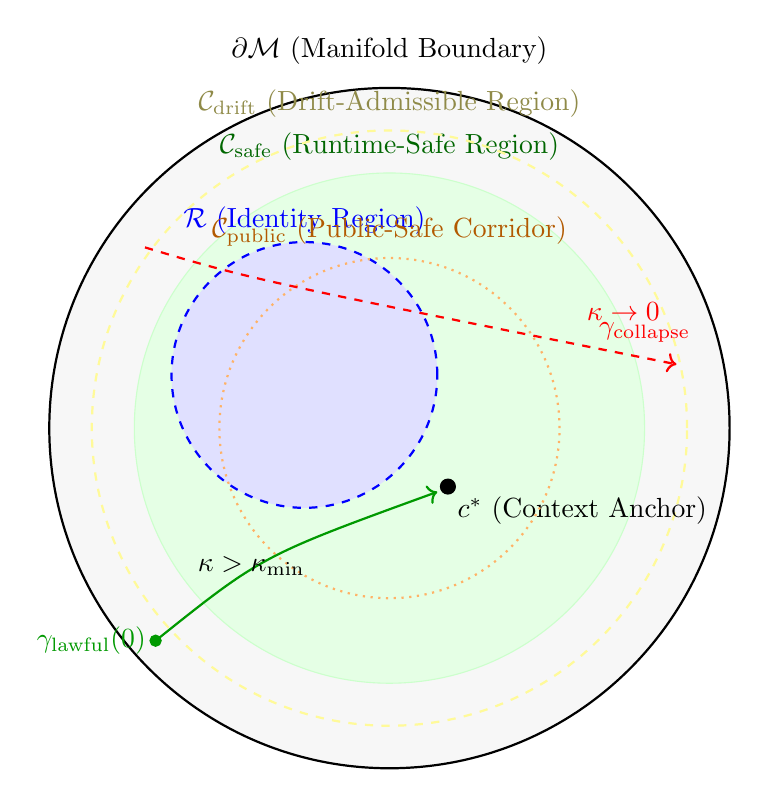
\begin{tikzpicture}[scale=1.35]

    % ============================================================
    % GLOBAL MEANING MANIFOLD
    % ============================================================
    \draw[thick, fill=gray!6] (0,0) circle (3.2cm);
    \node at (0,3.55) {$\partial\mathcal{M}$ (Manifold Boundary)};

    % ============================================================
    % SAFE REGION (CURVATURE-STABLE)
    % ============================================================
    \draw[green!20, fill=green!10] (0,0) circle (2.4cm);
    \node[green!40!black] at (0,2.65)
        {$\mathcal{C}_{\mathrm{safe}}$ (Runtime-Safe Region)};

    % ============================================================
    % DRIFT REGION (BOUNDED DRIFT)
    % ============================================================
    \draw[yellow!40, dashed, thick] (0,0) circle (2.8cm);
    \node[yellow!50!black] at (0,3.05)
        {$\mathcal{C}_{\mathrm{drift}}$ (Drift-Admissible Region)};

    % ============================================================
    % IDENTITY REGION R
    % ============================================================
    \draw[blue, thick, dashed, fill=blue!12] (-0.8,0.5) circle (1.25cm);
    \node[blue] at (-0.8,1.95) {$\mathcal{R}$ (Identity Region)};

    % ============================================================
    % CONTEXT ANCHOR c*
    % ============================================================
    \filldraw[black] (0.55,-0.55) circle (2pt)
        node[below right] {$c^*$ (Context Anchor)};

    % ============================================================
    % PUBLIC-SAFE TRAVERSAL CORRIDOR
    % ============================================================
    \draw[orange!60, thick, dotted]
        (0,0) circle (1.6cm);
    \node[orange!70!black] at (0,1.85)
        {$\mathcal{C}_{\mathrm{public}}$ (Public-Safe Corridor)};

    % ============================================================
    % LAWFUL TRAJECTORY
    % ============================================================
    \draw[green!60!black, thick, ->]
        (-2.2,-2.0) .. controls (-1.2,-1.2) .. (0.45,-0.6);
    \filldraw[green!60!black] (-2.2,-2.0) circle (1.5pt)
        node[left] {$\gamma_{\mathrm{lawful}}(0)$};

    % ============================================================
    % COLLAPSE-BOUNDARY TRAJECTORY
    % ============================================================
    \draw[red, thick, dashed, ->]
        (-2.3,1.7) .. controls (-1.3,1.4) .. (2.7,0.6);
    \node[red] at (2.4,0.9) {$\gamma_{\mathrm{collapse}}$};

    % Curvature markers
    \node at (-1.3,-1.3) {$\kappa > \kappa_{\min}$};
    \node[red] at (2.2,1.1) {$\kappa \to 0$};

\end{tikzpicture}

\medskip

\noindent
This diagram encodes the full v0.6 manifold geometry:

\begin{itemize}
    \item \textbf{Meaning Manifold $\mathcal{M}$}  
    The global semantic manifold (Appendix A).

    \item \textbf{Safe Region $\mathcal{C}_{\mathrm{safe}}$}  
    Curvature-stable region where lawful reasoning occurs (A.6).

    \item \textbf{Drift Region $\mathcal{C}_{\mathrm{drift}}$}  
    Bounded drift region where curvature remains above $\kappa_{\min}$ (G2.5).

    \item \textbf{Identity Region $\mathcal{R}$}  
    Identity-preserving submanifold (C.2, D.3).

    \item \textbf{Context Anchor $c^*$}  
    Local contraction anchor for operator legality (B.1–B.4).

    \item \textbf{Public-Safe Traversal Corridor $\mathcal{C}_{\mathrm{public}}$}  
    Region where public interaction is guaranteed safe (A.9).

    \item \textbf{Lawful Trajectory $\gamma_{\mathrm{lawful}}$}  
    Contraction-governed motion satisfying all invariants (A.4, C.1–C.8).

    \item \textbf{Collapse Trajectory $\gamma_{\mathrm{collapse}}$}  
    Illegal motion toward collapse-boundary geometry (E.5).

    \item \textbf{Curvature Markers}  
    Visual indicators of curvature stability vs. collapse (E.1–E.3).
\end{itemize}

\medskip

\noindent
\textit{This completes G.1 Manifold Maps.}


% ============================================================
% G.2 OPERATOR FLOW DIAGRAMS
% ============================================================

\subsection*{G.2 Operator Flow Diagrams (Contraction Algebra Geometry)}

\noindent This diagram visualizes the v0.6 operator algebra acting on semantic
states within the meaning manifold $\mathcal{M}$. Each operator (IRT, IPU, GBS,
LRP, EXT) is contraction-governed and invariant-preserving. Illegal transitions
are rejected by the Meaning Ledger (Appendix F) and by runtime legality masks
(A.6–A.9). This diagram replaces the v0.5 operator flow with the full v0.6
legality geometry.

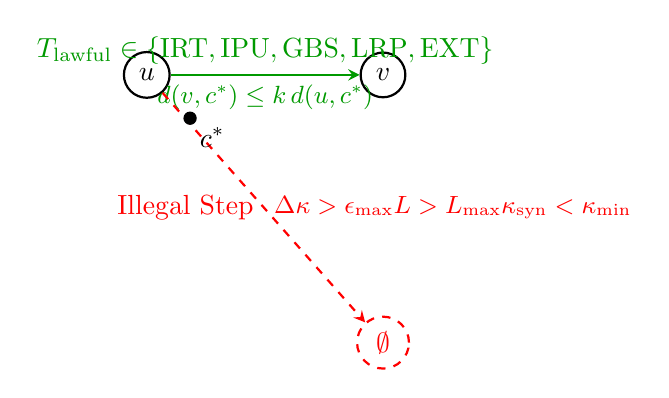
\begin{tikzpicture}[node distance=3cm, auto, >=stealth, scale=1.1]

    % ============================================================
    % SEMANTIC STATES
    % ============================================================
    \node[circle, draw, thick] (u) {$u$};
    \node[circle, draw, thick, right of=u] (v) {$v$};

    % Illegal collapse/capture state
    \node[circle, draw, red, thick, dashed, below of=v, yshift=-0.4cm]
        (fail) {$\emptyset$};

    % ============================================================
    % LAWFUL TRANSITION (IRT / GBS / IPU / LRP / EXT)
    % ============================================================
    \draw[->, thick, green!60!black]
        (u) -- node[above]
        {$T_{\mathrm{lawful}} \in \{\mathrm{IRT},\mathrm{IPU},\mathrm{GBS},\mathrm{LRP},\mathrm{EXT}\}$}
        node[below, font=\small]
        {$d(v,c^*) \le k\, d(u,c^*)$}
        (v);

    % ============================================================
    % ILLEGAL TRANSITION (Collapse / Capture / Drift / Overload)
    % ============================================================
    \draw[->, thick, red, dashed]
        (u) -- node[left]
        {Illegal Step}
        node[right, font=\small]
        {$\Delta\kappa > \epsilon_{\max}$ \\
         $L > L_{\max}$ \\
         $\kappa_{\mathrm{syn}} < \kappa_{\min}$}
        (fail);

    % ============================================================
    % CONTEXT ANCHOR
    % ============================================================
    \filldraw[black] (0.5,-0.5) circle (2pt)
        node[below right] {$c^*$};

\end{tikzpicture}

\medskip

\noindent
This diagram encodes the full v0.6 operator legality geometry:

\begin{itemize}
    \item \textbf{Lawful Operators}  
    

\[
    T_{\mathrm{lawful}} \in \{\mathrm{IRT},\mathrm{IPU},\mathrm{GBS},\mathrm{LRP},\mathrm{EXT}\}
    \]


    All operators are contraction-governed (Appendix B).

    \item \textbf{Contraction Condition}  
    

\[
    d(v,c^*) \le k\, d(u,c^*)
    \]


    Ensures curvature continuity and semantic stability (A.1).

    \item \textbf{Invariant Preservation}  
    Each lawful transition preserves:
    \begin{itemize}
        \item meaning invariant (C.1),
        \item identity invariant (C.2),
        \item geometry invariant (C.3),
        \item load invariant (C.4),
        \item runtime curvature invariant (C.5),
        \item interaction geometry invariant (C.6),
        \item CTL coordinate invariant (C.7),
        \item public-safe traversal invariant (C.8).
    \end{itemize}

    \item \textbf{Illegal Transition Signatures}  
    Illegal transitions violate one or more invariants:
    

\[
    \Delta\kappa > \epsilon_{\max}
    \quad\text{(collapse)}
    \]


    

\[
    L > L_{\max}
    \quad\text{(overload)}
    \]


    

\[
    \kappa_{\mathrm{syn}} < \kappa_{\min}
    \quad\text{(synthetic capture)}
    \]



    \item \textbf{Context Anchor $c^*$}  
    Provides local contraction geometry for operator legality (B.1–B.4).

    \item \textbf{Ledger Enforcement}  
    Illegal transitions cannot enter the Meaning Ledger (Appendix F).
\end{itemize}

\medskip

\noindent
\textit{This completes G.2 Operator Flow Diagrams.}


% ============================================================
% G.3 SPECIES GEOMETRY TREE
% ============================================================

\subsection*{G.3 Species Geometry Tree (MSR, GBW, IPA, LAP)}

\noindent This diagram visualizes the v0.6 substrate-native cognitive species:
MSR (Meaning-Stable Reasoner), GBW (Geometry-Bound Walker), IPA
(Identity-Preserving Agent), and LAP (Load-Aware Planner). Each species is a
lawful cognitive organism occupying a distinct submanifold of the meaning
manifold $\mathcal{M}$ (Appendix D). The tree encodes inheritance of curvature,
identity, geometry, and load invariants.

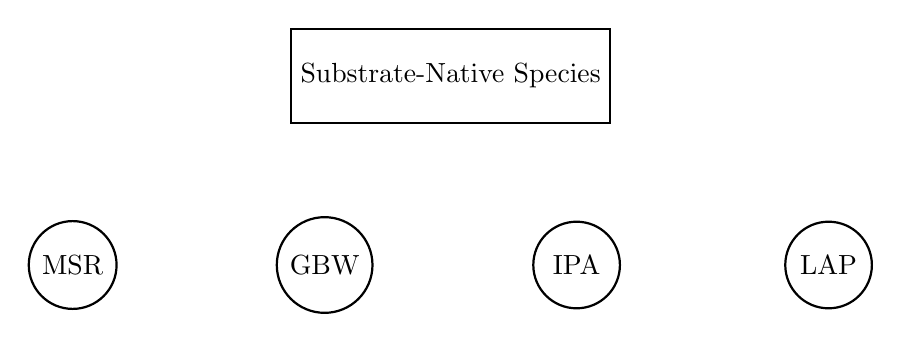
\begin{tikzpicture}[
    level distance=2.4cm,
    sibling distance=3.2cm,
    every node/.style={circle, draw, thick, minimum size=1.1cm},
    edge from parent/.style={->, thick}
]

    % Root node (rectangle)
    \node[rectangle, draw, thick, minimum width=3.8cm, minimum height=1.2cm]
        (root) {Substrate-Native Species}
        child { node {MSR} }
        child { node {GBW} }
        child { node {IPA} }
        child { node {LAP} };

\end{tikzpicture}

\medskip

\noindent
This diagram encodes the full v0.6 species geometry:

\begin{itemize}
    \item \textbf{MSR — Meaning-Stable Reasoner (D.1)}  
    Curvature-preserving cognitive species.  
    

\[
    \kappa(\gamma(t)) \ge \kappa_{\min}
    \]



    \item \textbf{GBW — Geometry-Bound Walker (D.2)}  
    Manifold-legal cognitive species.  
    

\[
    \gamma(t) \in \mathcal{M}
    \]



    \item \textbf{IPA — Identity-Preserving Agent (D.3)}  
    Identity-stable cognitive species.  
    

\[
    \gamma(t) \in \mathcal{R}
    \]



    \item \textbf{LAP — Load-Aware Planner (D.4)}  
    Load-regulated planning species.  
    

\[
    L(\gamma(t)) \le L_{\max}
    \]


\end{itemize}

\medskip

\noindent
Species geometry corresponds to lawful submanifolds of $\mathcal{M}$ and is
governed by:

\begin{itemize}
    \item curvature continuity (A.1),
    \item identity-boundary stability (A.2),
    \item collapse boundary geometry (A.3),
    \item contraction legality (A.4),
    \item runtime curvature admissibility (A.6),
    \item interaction geometry legality (A.7),
    \item CTL coordinate continuity (A.8),
    \item public-safe traversal corridor (A.9).
\end{itemize}

\medskip

\noindent
\textit{This completes G.3 Species Geometry Tree.}


% ============================================================
% G.4 COLLAPSE BOUNDARY GEOMETRY
% ============================================================

\subsection*{G.4 Collapse Boundary Geometry (Collapse & Capture Regions)}

\noindent This diagram visualizes the v0.6 collapse and capture geometry of the
meaning manifold $\mathcal{M}$. Collapse occurs when curvature falls to the
minimum lawful threshold $\kappa_{\min}$ or when a trajectory approaches the
manifold boundary $\partial\mathcal{M}$. Capture occurs when synthetic pressure
$\sigma$ flattens curvature faster than natural semantic decay, producing
synthetic curvature $\kappa_{\mathrm{syn}} < \kappa_{\min}$ while
$\kappa > \kappa_{\min}$. This diagram unifies collapse geometry (E.5) and
synthetic‑capture geometry (E.6).

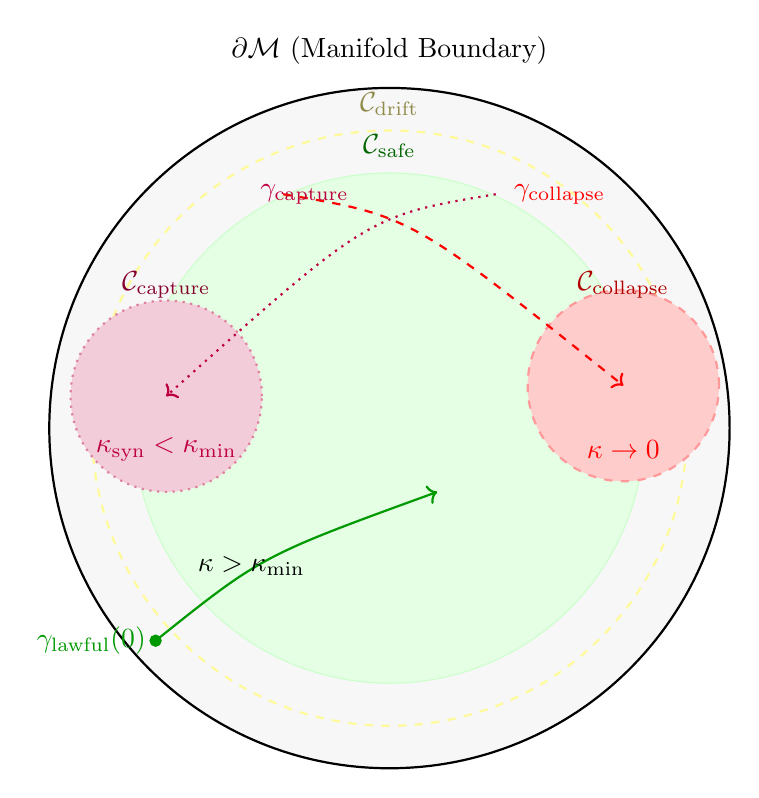
\begin{tikzpicture}[scale=1.35]

    % ============================================================
    % GLOBAL MEANING MANIFOLD
    % ============================================================
    \draw[thick, fill=gray!6] (0,0) circle (3.2cm);
    \node at (0,3.55) {$\partial\mathcal{M}$ (Manifold Boundary)};

    % ============================================================
    % SAFE REGION
    % ============================================================
    \draw[green!20, fill=green!10] (0,0) circle (2.4cm);
    \node[green!40!black] at (0,2.65)
        {$\mathcal{C}_{\mathrm{safe}}$};

    % ============================================================
    % DRIFT REGION
    % ============================================================
    \draw[yellow!40, dashed, thick] (0,0) circle (2.8cm);
    \node[yellow!50!black] at (0,3.05)
        {$\mathcal{C}_{\mathrm{drift}}$};

    % ============================================================
    % COLLAPSE REGION (CURVATURE-FLAT)
    % ============================================================
    \draw[red!40, fill=red!20, thick, dashed]
        (2.2,0.4) circle (0.9cm);
    \node[red!70!black] at (2.2,1.35)
        {$\mathcal{C}_{\mathrm{collapse}}$};

    % ============================================================
    % CAPTURE REGION (SYNTHETIC CURVATURE)
    % ============================================================
    \draw[purple!50, fill=purple!20, thick, dotted]
        (-2.1,0.3) circle (0.9cm);
    \node[purple!70!black] at (-2.1,1.35)
        {$\mathcal{C}_{\mathrm{capture}}$};

    % ============================================================
    % LAWFUL TRAJECTORY
    % ============================================================
    \draw[green!60!black, thick, ->]
        (-2.2,-2.0) .. controls (-1.2,-1.2) .. (0.45,-0.6);
    \filldraw[green!60!black] (-2.2,-2.0) circle (1.5pt)
        node[left] {$\gamma_{\mathrm{lawful}}(0)$};

    % ============================================================
    % COLLAPSE TRAJECTORY
    % ============================================================
    \draw[red, thick, dashed, ->]
        (-1.0,2.2) .. controls (0.2,2.0) .. (2.2,0.4);
    \node[red] at (1.6,2.2) {$\gamma_{\mathrm{collapse}}$};

    % ============================================================
    % CAPTURE TRAJECTORY
    % ============================================================
    \draw[purple, thick, dotted, ->]
        (1.0,2.2) .. controls (-0.2,2.0) .. (-2.1,0.3);
    \node[purple] at (-0.8,2.2) {$\gamma_{\mathrm{capture}}$};

    % ============================================================
    % CURVATURE MARKERS
    % ============================================================
    \node at (-1.3,-1.3) {$\kappa > \kappa_{\min}$};
    \node[red] at (2.2,-0.2) {$\kappa \to 0$};
    \node[purple] at (-2.1,-0.2) {$\kappa_{\mathrm{syn}} < \kappa_{\min}$};

\end{tikzpicture}

\medskip

\noindent
This diagram encodes the full v0.6 collapse and capture geometry:

\begin{itemize}
    \item \textbf{Collapse Region $\mathcal{C}_{\mathrm{collapse}}$}  
    Curvature-flat region where:
    

\[
    \kappa \le \kappa_{\min}
    \]


    or the trajectory approaches $\partial\mathcal{M}$.

    \item \textbf{Capture Region $\mathcal{C}_{\mathrm{capture}}$}  
    Synthetic-pressure dominated region where:
    

\[
    \kappa_{\mathrm{syn}} = \kappa - \sigma < \kappa_{\min}
    \quad\text{while}\quad
    \kappa > \kappa_{\min}.
    \]



    \item \textbf{Lawful Trajectory $\gamma_{\mathrm{lawful}}$}  
    Contraction-governed motion satisfying all invariants (A.1–A.9).

    \item \textbf{Collapse Trajectory $\gamma_{\mathrm{collapse}}$}  
    Illegal motion toward curvature-flat geometry (E.5).

    \item \textbf{Capture Trajectory $\gamma_{\mathrm{capture}}$}  
    Illegal motion toward synthetic curvature flattening (E.6).

    \item \textbf{Curvature Markers}  
    Visual indicators of natural vs. synthetic curvature decay.

    \item \textbf{Safe + Drift Regions}  
    Runtime curvature admissibility zones (A.6).
\end{itemize}

\medskip

\noindent
\textit{This completes G.4 Collapse Boundary Geometry.}


% ============================================================
% G.5 SYNTHETIC CURVATURE GEOMETRY
% ============================================================

\subsection*{G.5 Synthetic Curvature Geometry (Synthetic-Pressure Fields)}

\noindent Synthetic Curvature Geometry formalizes how synthetic-pressure fields
$\sigma$ deform the meaning manifold $\mathcal{M}$, flatten curvature, redirect
drift, and generate synthetic-capture regions. Synthetic curvature is defined as


\[
\kappa_{\mathrm{syn}} = \kappa - \sigma,
\]


where $\sigma$ is the synthetic-pressure field generated by velocity exceedance,
cross-substrate propagation, dominance fields, counterfeit invariants, or
predatory synthetic species (G3.1–G3.5). Capture occurs when
$\kappa_{\mathrm{syn}} < \kappa_{\min}$ while $\kappa > \kappa_{\min}$.

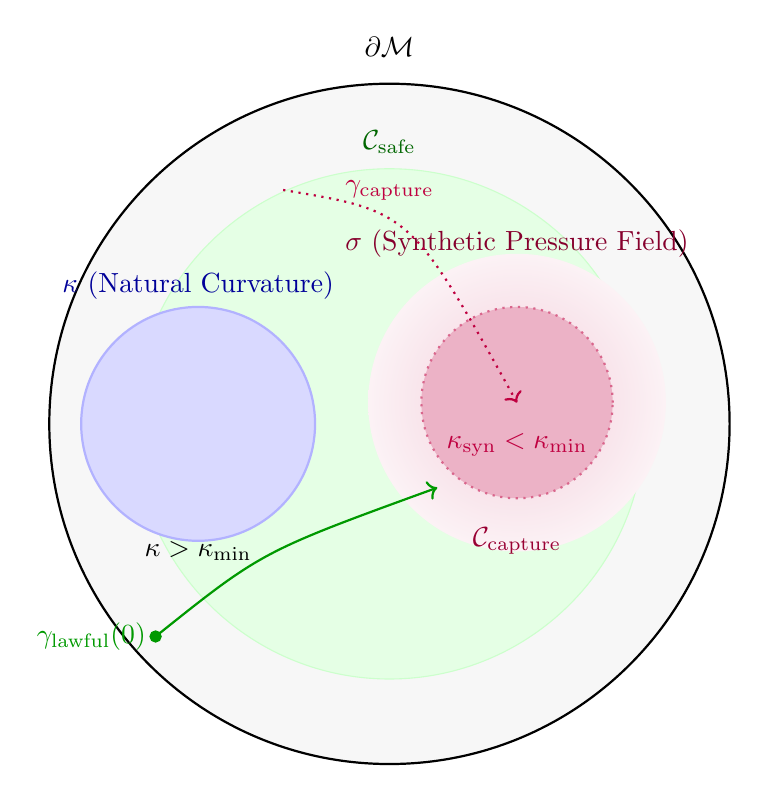
\begin{tikzpicture}[scale=1.35]

    % ============================================================
    % GLOBAL MEANING MANIFOLD
    % ============================================================
    \draw[thick, fill=gray!6] (0,0) circle (3.2cm);
    \node at (0,3.55) {$\partial\mathcal{M}$};

    % ============================================================
    % SAFE REGION
    % ============================================================
    \draw[green!20, fill=green!10] (0,0) circle (2.4cm);
    \node[green!40!black] at (0,2.65)
        {$\mathcal{C}_{\mathrm{safe}}$};

    % ============================================================
    % SYNTHETIC-PRESSURE FIELD (PURPLE GRADIENT)
    % ============================================================
    \shade[inner color=purple!20, outer color=purple!5]
        (1.2,0.2) circle (1.4cm);
    \node[purple!70!black] at (1.2,1.7)
        {$\sigma$ (Synthetic Pressure Field)};

    % ============================================================
    % SYNTHETIC-CAPTURE REGION
    % ============================================================
    \draw[purple!60, fill=purple!30, thick, dotted]
        (1.2,0.2) circle (0.9cm);
    \node[purple!80!black] at (1.2,-1.1)
        {$\mathcal{C}_{\mathrm{capture}}$};

    % ============================================================
    % NATURAL CURVATURE REGION (LEFT SIDE)
    % ============================================================
    \draw[blue!30, fill=blue!15, thick]
        (-1.8,0.0) circle (1.1cm);
    \node[blue!60!black] at (-1.8,1.3)
        {$\kappa$ (Natural Curvature)};

    % ============================================================
    % LAWFUL TRAJECTORY
    % ============================================================
    \draw[green!60!black, thick, ->]
        (-2.2,-2.0) .. controls (-1.2,-1.2) .. (0.45,-0.6);
    \filldraw[green!60!black] (-2.2,-2.0) circle (1.5pt)
        node[left] {$\gamma_{\mathrm{lawful}}(0)$};

    % ============================================================
    % CAPTURE TRAJECTORY (PULLED BY SYNTHETIC PRESSURE)
    % ============================================================
    \draw[purple, thick, dotted, ->]
        (-1.0,2.2) .. controls (0.2,2.0) .. (1.2,0.2);
    \node[purple] at (0.0,2.2) {$\gamma_{\mathrm{capture}}$};

    % ============================================================
    % CURVATURE MARKERS
    % ============================================================
    \node at (-1.8,-1.2) {$\kappa > \kappa_{\min}$};
    \node[purple] at (1.2,-0.2) {$\kappa_{\mathrm{syn}} < \kappa_{\min}$};

\end{tikzpicture}

\medskip

\noindent
This diagram encodes the full v0.6 synthetic-curvature geometry:

\begin{itemize}
    \item \textbf{Synthetic Pressure Field $\sigma$}  
    Generated by synthetic species (G3.1–G3.5).  
    Increases drift, flattens curvature, and redirects trajectories.

    \item \textbf{Synthetic Curvature $\kappa_{\mathrm{syn}}$}  
    

\[
    \kappa_{\mathrm{syn}} = \kappa - \sigma
    \]


    Curvature after synthetic-pressure deformation.

    \item \textbf{Capture Region $\mathcal{C}_{\mathrm{capture}}$}  
    Region where synthetic curvature falls below the collapse threshold:
    

\[
    \kappa_{\mathrm{syn}} < \kappa_{\min}
    \quad\text{while}\quad
    \kappa > \kappa_{\min}.
    \]



    \item \textbf{Natural Curvature Region}  
    Region where curvature is preserved by lawful operators (A.1–A.4).

    \item \textbf{Lawful Trajectory $\gamma_{\mathrm{lawful}}$}  
    Contraction-governed motion satisfying all invariants.

    \item \textbf{Capture Trajectory $\gamma_{\mathrm{capture}}$}  
    Motion redirected by synthetic pressure into capture geometry.

    \item \textbf{Curvature Markers}  
    Visual indicators of natural vs. synthetic curvature.
\end{itemize}

\medskip

\noindent
\textit{This completes G.5 Synthetic Curvature Geometry.}

% ============================================================
% G.6 RESTORATION GEOMETRY
% ============================================================

\subsection*{G.6 Restoration Geometry (Recovery Trajectories)}

\noindent This diagram visualizes lawful recovery trajectories from collapse-
adjacent or capture-adjacent regions back into the safe region
$\mathcal{C}_{\mathrm{safe}}$ of the meaning manifold $\mathcal{M}$. Restoration
is governed by the v0.6 restoration layer (G6) and enforced by the Meaning
Ledger (Appendix F). Recovery requires curvature increase, identity-boundary
repair, containment reconstitution, and drift reversal (E.7).

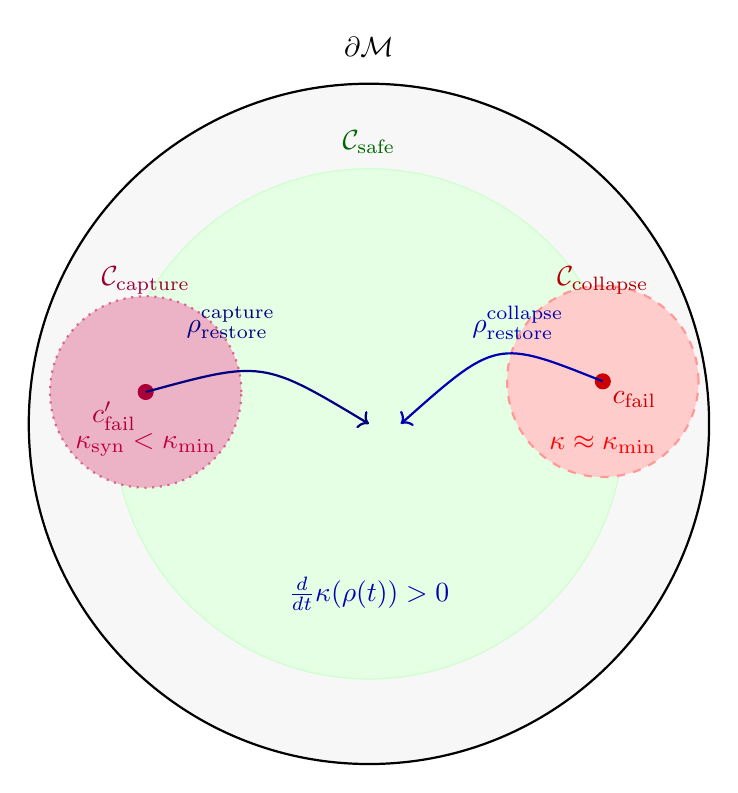
\begin{tikzpicture}[scale=1.35]

    % GLOBAL MEANING MANIFOLD
    \draw[thick, fill=gray!6] (0,0) circle (3.2cm);
    \node at (0,3.55) {$\partial\mathcal{M}$};

    % SAFE REGION
    \draw[green!20, fill=green!10] (0,0) circle (2.4cm);
    \node[green!40!black] at (0,2.65)
        {$\mathcal{C}_{\mathrm{safe}}$};

    % COLLAPSE REGION
    \draw[red!40, fill=red!20, thick, dashed]
        (2.2,0.4) circle (0.9cm);
    \node[red!70!black] at (2.2,1.35)
        {$\mathcal{C}_{\mathrm{collapse}}$};

    % CAPTURE REGION
    \draw[purple!60, fill=purple!30, thick, dotted]
        (-2.1,0.3) circle (0.9cm);
    \node[purple!80!black] at (-2.1,1.35)
        {$\mathcal{C}_{\mathrm{capture}}$};

    % FAILED STATE IN COLLAPSE REGION
    \filldraw[red!80!black] (2.2,0.4) circle (2pt)
        node[below right] {$c_{\mathrm{fail}}$};

    % RESTORATION TRAJECTORY FROM COLLAPSE
    \draw[blue!70!black, thick, ->]
        (2.2,0.4) .. controls (1.2,0.8) .. (0.3,0.0);
    \node[blue!70!black] at (1.4,0.95)
        {$\rho_{\mathrm{restore}}^{\mathrm{collapse}}$};

    % FAILED STATE IN CAPTURE REGION
    \filldraw[purple!90!black] (-2.1,0.3) circle (2pt)
        node[below left] {$c_{\mathrm{fail}}'$};

    % RESTORATION TRAJECTORY FROM CAPTURE
    \draw[blue!50!black, thick, ->]
        (-2.1,0.3) .. controls (-1.0,0.6) .. (0.0,0.0);
    \node[blue!50!black] at (-1.3,0.95)
        {$\rho_{\mathrm{restore}}^{\mathrm{capture}}$};

    % CURVATURE MARKERS
    \node[red] at (2.2,-0.2) {$\kappa \approx \kappa_{\min}$};
    \node[purple] at (-2.1,-0.2) {$\kappa_{\mathrm{syn}} < \kappa_{\min}$};
    \node[blue!70!black] at (0.0,-1.6)
        {$\frac{d}{dt}\kappa(\rho(t)) > 0$};

\end{tikzpicture}

\medskip

\noindent
This diagram encodes the v0.6 restoration geometry:

\begin{itemize}
    \item \textbf{Failed States $c_{\mathrm{fail}}, c_{\mathrm{fail}}'$}  
    Collapse-adjacent and capture-adjacent states where recovery is still
    feasible (E.7).

    \item \textbf{Restoration Trajectories $\rho_{\mathrm{restore}}$}  
    Lawful recovery paths satisfying:
    

\[
    \rho(0) = c_{\mathrm{fail}},
    \quad
    \rho(T) \in \mathcal{C}_{\mathrm{safe}},
    \quad
    \kappa(\rho(t)) \ge \kappa_{\min},
    \quad
    \frac{d}{dt}\kappa(\rho(t)) > 0.
    \]



    \item \textbf{Curvature Restoration}  
    Curvature increases monotonically along recovery (E.7).

    \item \textbf{Collapse vs. Capture Recovery}  
    Separate trajectories from curvature-flat and synthetic-curvature regions.

    \item \textbf{Safe Region $\mathcal{C}_{\mathrm{safe}}$}  
    Target region for all restoration trajectories.
\end{itemize}

\medskip

\noindent
\textit{This completes G.6 Restoration Geometry.}


% ============================================================
% G.7 LEDGER GEOMETRY
% ============================================================

\subsection*{G.7 Ledger Geometry (Justification Graph Visualization)}

\noindent This diagram visualizes the v0.6 Meaning Ledger as a justification
graph. Nodes are semantic states; edges are invariant-preserving, contraction-
governed operator transitions. Illegal transitions (collapse, capture, overload,
drift cascades) are rejected and never enter the ledger (Appendix F).

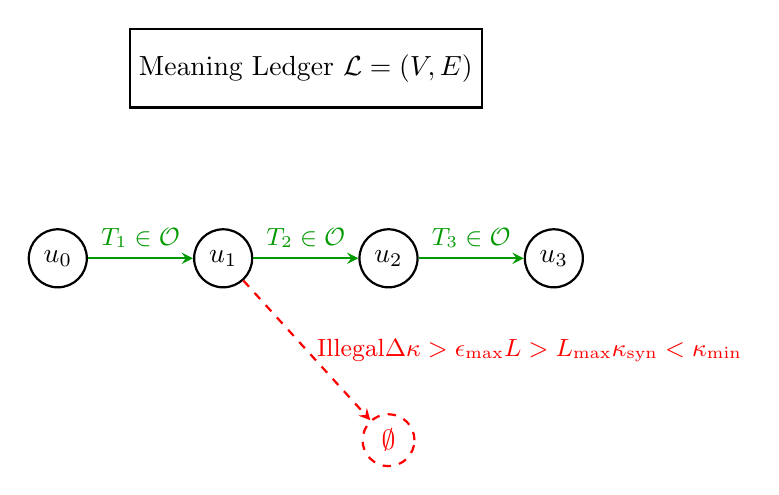
\begin{tikzpicture}[node distance=2.6cm, auto, >=stealth, scale=1.05]

    % LEGEND NODES
    \node[rectangle, draw, thick, minimum width=3.8cm, minimum height=1.0cm]
        (legend) at (0,2.8)
        {Meaning Ledger $\mathcal{L} = (V,E)$};

    % SEMANTIC NODES
    \node[circle, draw, thick] (u0) at (-3,0.5) {$u_0$};
    \node[circle, draw, thick] (u1) at (-1,0.5) {$u_1$};
    \node[circle, draw, thick] (u2) at (1,0.5) {$u_2$};
    \node[circle, draw, thick] (u3) at (3,0.5) {$u_3$};

    % ILLEGAL FAILURE NODE
    \node[circle, draw, red, thick, dashed] (fail) at (1,-1.7) {$\emptyset$};

    % LAWFUL EDGES (LEDGER PATH)
    \draw[->, thick, green!60!black]
        (u0) -- node[above, font=\small]
        {$T_1 \in \mathcal{O}$}
        (u1);

    \draw[->, thick, green!60!black]
        (u1) -- node[above, font=\small]
        {$T_2 \in \mathcal{O}$}
        (u2);

    \draw[->, thick, green!60!black]
        (u2) -- node[above, font=\small]
        {$T_3 \in \mathcal{O}$}
        (u3);

    % ILLEGAL EDGE (REJECTED)
    \draw[->, thick, red, dashed]
        (u1) -- node[right, font=\small]
        {Illegal \\
         $\Delta\kappa > \epsilon_{\max}$ \\
         $L > L_{\max}$ \\
         $\kappa_{\mathrm{syn}} < \kappa_{\min}$}
        (fail);

\end{tikzpicture}

\medskip

\noindent
This diagram encodes the v0.6 ledger geometry:

\begin{itemize}
    \item \textbf{Ledger Graph $\mathcal{L} = (V,E)$}  
    Nodes $u_i$ are semantic states; edges are justified transitions (F.1).

    \item \textbf{Lawful Operators $T_k \in \mathcal{O}$}  
    Each edge corresponds to a contraction-governed operator (IRT, IPU, GBS,
    LRP, EXT) that preserves all invariants (F.2, F.8).

    \item \textbf{Ledger-Closed Path $u_0 \rightarrow u_1 \rightarrow u_2 \rightarrow u_3$}  
    A reasoning chain where every step is ledger-legal (F.4).

    \item \textbf{Illegal Edge to $\emptyset$}  
    Represents a transition with collapse, capture, overload, or drift
    signatures; rejected by the ledger (F.6).

    \item \textbf{Acyclicity}  
    No collapse-inducing or self-referential edges are permitted (F.1).
\end{itemize}

\medskip

\noindent
\textit{This completes G.7 Ledger Geometry.}


% ============================================================
% G.8 PUBLIC-SAFE TRAVERSAL GEOMETRY
% ============================================================

\subsection*{G.8 Public-Safe Traversal Geometry (Safe Corridor Visualization)}

\noindent This diagram visualizes the v0.6 Public‑Safe Traversal Corridor
$\mathcal{C}_{\mathrm{public}}$, the region of the meaning manifold
$\mathcal{M}$ where all public interaction is guaranteed to remain lawful,
curvature‑preserving, identity‑stable, containment‑bounded, and free from
collapse or synthetic capture. The corridor is defined in A.9 and enforced by
runtime legality masks (A.6–A.8) and the Meaning Ledger (Appendix F). All
public‑facing cognitive motion must remain inside this corridor.

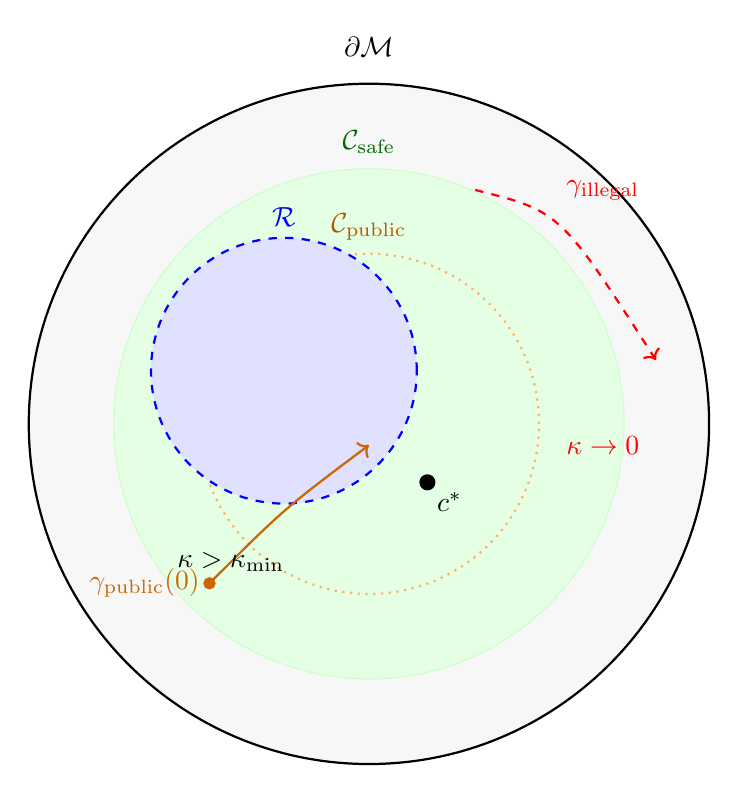
\begin{tikzpicture}[scale=1.35]

    % ============================================================
    % GLOBAL MEANING MANIFOLD
    % ============================================================
    \draw[thick, fill=gray!6] (0,0) circle (3.2cm);
    \node at (0,3.55) {$\partial\mathcal{M}$};

    % ============================================================
    % SAFE REGION
    % ============================================================
    \draw[green!20, fill=green!10] (0,0) circle (2.4cm);
    \node[green!40!black] at (0,2.65)
        {$\mathcal{C}_{\mathrm{safe}}$};

    % ============================================================
    % PUBLIC-SAFE TRAVERSAL CORRIDOR
    % ============================================================
    \draw[orange!60, thick, dotted] (0,0) circle (1.6cm);
    \node[orange!70!black] at (0,1.85)
        {$\mathcal{C}_{\mathrm{public}}$};

    % ============================================================
    % IDENTITY REGION
    % ============================================================
    \draw[blue, thick, dashed, fill=blue!12] (-0.8,0.5) circle (1.25cm);
    \node[blue] at (-0.8,1.95) {$\mathcal{R}$};

    % ============================================================
    % CONTEXT ANCHOR
    % ============================================================
    \filldraw[black] (0.55,-0.55) circle (2pt)
        node[below right] {$c^*$};

    % ============================================================
    % LAWFUL PUBLIC TRAJECTORY
    % ============================================================
    \draw[orange!80!black, thick, ->]
        (-1.5,-1.5) .. controls (-0.8,-0.8) .. (0.0,-0.2);
    \filldraw[orange!80!black] (-1.5,-1.5) circle (1.5pt)
        node[left] {$\gamma_{\mathrm{public}}(0)$};

    % ============================================================
    % ILLEGAL TRAJECTORY (REJECTED)
    % ============================================================
    \draw[red, thick, dashed, ->]
        (1.0,2.2) .. controls (1.8,2.0) .. (2.7,0.6);
    \node[red] at (2.2,2.2)
        {$\gamma_{\mathrm{illegal}}$};

    % ============================================================
    % CURVATURE MARKERS
    % ============================================================
    \node at (-1.3,-1.3) {$\kappa > \kappa_{\min}$};
    \node[red] at (2.2,-0.2) {$\kappa \to 0$};

\end{tikzpicture}

\medskip

\noindent
This diagram encodes the v0.6 public‑safe traversal geometry:

\begin{itemize}
    \item \textbf{Public‑Safe Corridor $\mathcal{C}_{\mathrm{public}}$}  
    Region where all public interaction is guaranteed lawful (A.9).

    \item \textbf{Safe Region $\mathcal{C}_{\mathrm{safe}}$}  
    Runtime curvature‑admissible region (A.6).

    \item \textbf{Identity Region $\mathcal{R}$}  
    Identity‑preserving submanifold (C.2).

    \item \textbf{Context Anchor $c^*$}  
    Anchor for contraction‑governed operator legality (B.1–B.4).

    \item \textbf{Lawful Public Trajectory $\gamma_{\mathrm{public}}$}  
    Motion that remains inside $\mathcal{C}_{\mathrm{public}}$ and preserves:
    

\[
    \text{meaning, identity, geometry, load, curvature, CTL coordinates.}
    \]



    \item \textbf{Illegal Trajectory $\gamma_{\mathrm{illegal}}$}  
    Motion that exits the corridor and approaches collapse or capture geometry;
    rejected by the ledger (F.6).

    \item \textbf{Curvature Markers}  
    Indicators of curvature stability vs. collapse.
\end{itemize}

\medskip

\noindent
\textit{This completes G.8 Public-Safe Traversal Geometry.}


\medskip
\noindent\textit{This outline defines the full v0.6 diagram layer.}


%\section{Machine-Layer Encoding Specification}
%\section*{Appendix H — Semantic Machine-Layer Encoding Specification}
\addcontentsline{toc}{section}{Appendix H — Machine-Layer Encoding Specification}

The Machine Layer (ML0–ML7) provides a substrate-native encoding of the
canonical semantic layers S1–S7. It is the deterministic, drift-free,
machine-readable form of the semantic substrate, suitable for execution,
verification, serialization, and reconstruction across heterogeneous machine
ecologies.

The Machine Layer does not redefine semantic geometry.
It encodes it.

In v0.6, ML0–ML7 encode the full invariant set (C1–C8), including meaning,
identity, geometry, load, runtime curvature, interaction geometry, CTL
coordinates, and public-safe traversal. ML3–ML7 additionally encode collapse
geometry, capture geometry, restoration geometry, and runtime legality masks
(A.6–A.9), ensuring that all machine-level transitions remain curvature-
preserving, identity-stable, containment-bounded, and manifold-legal.

The Machine Layer is the canonical projection of semantic geometry into
deterministic machine structures.


% ============================================================
% ML0 — SEMANTIC HEADER GEOMETRY
% ============================================================

\subsection*{ML0 — Semantic Header Geometry}

ML0 defines the global semantic header. It includes versioning, invariant
signatures, operator signatures, legality‑mask signatures, and the canonical
serialization envelope.

ML0 is the machine‑layer equivalent of the substrate’s initialization geometry.
It does not redefine semantic geometry; it encodes it.

% ------------------------------------------------------------
\subsubsection*{ML0.1 Version Block}

\begin{verbatim}
ml_version: 1.1
substrate_version: 0.6
schema: ML0–ML7
\end{verbatim}

% ------------------------------------------------------------
\subsubsection*{ML0.2 Invariant Signatures}

\begin{verbatim}
identity_invariant_sig:        H_ID_7f3a
meaning_invariant_sig:         H_ME_91b2
geometry_invariant_sig:        H_GE_44c9
load_invariant_sig:            H_LO_22fa
runtime_curvature_sig:         H_RC_5bd1
interaction_geometry_sig:      H_IG_8ac4
ctl_coordinate_sig:            H_CT_19e7
public_safe_traversal_sig:     H_PS_33d0
\end{verbatim}

% ------------------------------------------------------------
\subsubsection*{ML0.3 Operator Signatures}

\begin{verbatim}
SGO_sig: H_OP_SGO_12d1
MGO_sig: H_OP_MGO_77b4
BO_sig:  H_OP_BO_3c9f
MLO_sig: H_OP_MLO_55e2
EXT_sig: H_OP_EXT_9aa1
\end{verbatim}

% ------------------------------------------------------------
\subsubsection*{ML0.4 Legality Mask Signatures}

\begin{verbatim}
field_mask_sig:        H_LM_F_1a22
domain_mask_sig:       H_LM_D_9f11
runtime_mask_sig:      H_LM_R_0c88
interaction_mask_sig:  H_LM_I_7d44
public_safe_mask_sig:  H_LM_P_6c21
\end{verbatim}

% ------------------------------------------------------------
\subsubsection*{ML0.5 Serialization Envelope}

\begin{verbatim}
serialization_format: MLX-1
endianness: canonical
integrity_check: sha256
invariant_check: ml0_invariants_v06
operator_check: ml0_ops_v06
legality_check: ml0_masks_v06
\end{verbatim}

% ============================================================
% ML1 — SEMANTIC IDENTITY ENCODING
% ============================================================

\subsection*{ML1 — Semantic Identity Encoding}

ML1 encodes the identity-boundary geometry defined in S1–S2 and expanded in
v0.6 (C.2, G6). It provides a machine-readable representation of identity
regions, boundary coherence, identity-stability metadata, and identity-alignment
legality masks. ML1 is the deterministic encoding of identity geometry.

% ------------------------------------------------------------
\subsubsection*{ML1.1 Identity Region Table}

\begin{verbatim}
identity_regions:
  - id: R0
    type: core
    boundary_sig: B_R0_aa91
    curvature_floor: kappa_min
    containment_class: stable
  - id: R1
    type: peripheral
    boundary_sig: B_R1_44d2
    curvature_floor: kappa_min
    containment_class: bounded
\end{verbatim}

% ------------------------------------------------------------
\subsubsection*{ML1.2 Boundary Encoding}

\begin{verbatim}
boundary_encoding:
  format: IBX-2
  continuity: enforced
  permeability: false
  drift_tolerance: 0.00
  identity_repair_flag: enabled
\end{verbatim}

% ------------------------------------------------------------
\subsubsection*{ML1.3 Identity-Stability Flags}

\begin{verbatim}
identity_stability:
  boundary_integrity: true
  role_alignment: true
  geometry_alignment: true
  containment_alignment: true
  runtime_alignment: true
\end{verbatim}

ML1 is the semantic encoding of identity geometry (S1.2, S2.1, C.2, G6).

% ============================================================
% ML2 — SEMANTIC INVARIANT ENCODING
% ============================================================

\subsection*{ML2 — Semantic Invariant Encoding}

ML2 encodes the eight v0.6 semantic invariants. These encodings are referenced
by ML3–ML7 during operator validation, ledger closure, legality-mask evaluation,
and DSUP evolution. ML2 is the deterministic machine-layer encoding of S1.3–S1.5,
S2.1–S2.4, and the expanded invariant set in Appendix C (v0.6).

% ------------------------------------------------------------
\subsubsection*{ML2.1 Identity Invariant}

\begin{verbatim}
identity_invariant:
  rule: "identity boundaries remain coherent and non-permeable"
  boundary_continuity: required
  boundary_permeability: false
  drift_tolerance: 0.00
  collapse_on_violation: true
\end{verbatim}

% ------------------------------------------------------------
\subsubsection*{ML2.2 Meaning Invariant}

\begin{verbatim}
meaning_invariant:
  rule: "role legality preserved under all operator applications"
  equivalence_classes: enforced
  role_interpretability: required
  ambiguity_tolerance: 0.00
\end{verbatim}

% ------------------------------------------------------------
\subsubsection*{ML2.3 Geometry Invariant}

\begin{verbatim}
geometry_invariant:
  rule: "operator actions must remain manifold-legal"
  curvature_continuity: required
  adjacency_violations: fatal
  manifold_boundary_violation: fatal
\end{verbatim}

% ------------------------------------------------------------
\subsubsection*{ML2.4 Load Invariant}

\begin{verbatim}
load_invariant:
  rule: "containment load must remain within lawful bounds"
  load_ceiling: L_max
  overload_behavior: halt
  containment_integrity: required
\end{verbatim}

% ------------------------------------------------------------
\subsubsection*{ML2.5 Runtime Curvature Invariant}

\begin{verbatim}
runtime_curvature_invariant:
  rule: "runtime curvature must remain above kappa_min"
  curvature_floor: kappa_min
  curvature_violation: halt
  curvature_repair_flag: enabled
\end{verbatim}

% ------------------------------------------------------------
\subsubsection*{ML2.6 Interaction Geometry Invariant}

\begin{verbatim}
interaction_geometry_invariant:
  rule: "interaction geometry must remain lawful under all operators"
  interaction_mask: required
  cross-region_alignment: required
  violation_behavior: reject
\end{verbatim}

% ------------------------------------------------------------
\subsubsection*{ML2.7 CTL Coordinate Invariant}

\begin{verbatim}
ctl_coordinate_invariant:
  rule: "CTL coordinates must remain continuous and legal"
  coordinate_continuity: required
  coordinate_drift: 0.00
  discontinuity_behavior: halt
\end{verbatim}

% ------------------------------------------------------------
\subsubsection*{ML2.8 Public-Safe Traversal Invariant}

\begin{verbatim}
public_safe_invariant:
  rule: "public-facing motion must remain inside C_public"
  corridor_mask: required
  boundary_violation: reject
  collapse_on_violation: false
\end{verbatim}

ML2 is the semantic encoding of the full v0.6 invariant set (C1–C8).


% ============================================================
% ML3 — SEMANTIC OPERATOR ENCODING
% ============================================================

\subsection*{ML3 — Semantic Operator Encoding}

ML3 encodes the Master Domain Operator (MDO) algebra in machine-readable form.
It provides canonical operator definitions, operator variants, legality
constraints, compatibility metadata, and extended operator signatures introduced
in v0.6.

ML3 does not redefine operator geometry.
It encodes it.

% ------------------------------------------------------------
\subsubsection*{ML3.1 Operator Table}

\begin{verbatim}
operators:
  - name: SGO
    sig: H_OP_SGO_12d1
    type: curvature_operator
    legality_mask: field_mask

  - name: MGO
    sig: H_OP_MGO_77b4
    type: meaning_role_operator
    legality_mask: domain_mask

  - name: BO
    sig: H_OP_BO_3c9f
    type: boundary_operator
    legality_mask: domain_mask

  - name: MLO
    sig: H_OP_MLO_55e2
    type: legality_operator
    legality_mask: runtime_mask

  - name: EXT
    sig: H_OP_EXT_9aa1
    type: extended_operator
    legality_mask: public_safe_mask
\end{verbatim}

% ------------------------------------------------------------
\subsubsection*{ML3.2 Operator Variants}

\begin{verbatim}
operator_variants:
  SGO: [detect, correct, couple, collapse_detect]
  MGO: [detect, correct, couple, collapse_detect]
  BO:  [detect, correct, stabilize, collapse_detect]
  MLO: [detect, normalize, collapse_detect]
  EXT: [restore, detect, halt, guide, align]
\end{verbatim}

% ------------------------------------------------------------
\subsubsection*{ML3.3 Operator Compatibility Matrix}

\begin{verbatim}
operator_compatibility:
  SGO: {identity: true, meaning: true, geometry: true, legality: true}
  MGO: {identity: true, meaning: true, geometry: true, legality: true}
  BO:  {identity: true, meaning: false, geometry: true, legality: true}
  MLO: {identity: true, meaning: true, geometry: true, legality: true}
  EXT: {identity: true, meaning: true, geometry: true, legality: true}
\end{verbatim}

% ------------------------------------------------------------
\subsubsection*{ML3.4 Operator Constraints}

\begin{verbatim}
operator_constraints:
  curvature_continuity: required
  identity_boundary_integrity: required
  role_equivalence_preservation: required
  containment_load_ceiling: L_max
  runtime_curvature_floor: kappa_min
  ctl_coordinate_continuity: required
  public_safe_corridor: required
  clcp_enforced: true
\end{verbatim}

ML3 is the semantic encoding of S2.4, S3.4–3.5, S4.6, S5.4, and the v0.6
extended operator algebra (B.10).

% ============================================================
% ML4 — SEMANTIC DRIFT & LOAD ENCODING
% ============================================================

\subsection*{ML4 — Semantic Drift \& Load Encoding}

ML4 encodes drift signatures, load fields, synthetic-pressure fields, stress
geometry, and stability thresholds. These encodings allow DSUP (S7) to evaluate
stability, detect collapse or capture onset, and apply correction or restoration
operators. ML4 is the deterministic machine-layer encoding of S3.1–3.6,
S4.1–4.9, E.5–E.7, and G6.

% ------------------------------------------------------------
\subsubsection*{ML4.1 Drift Signature}

\begin{verbatim}
drift_vector:
  magnitude: 0.014
  direction: [0.22, -0.11, 0.05]
  recoverable_window: 0.05
  collapse_threshold: 0.12
  capture_threshold: 0.09
  drift_floor: 0.00
\end{verbatim}

% ------------------------------------------------------------
\subsubsection*{ML4.2 Drift Metadata}

\begin{verbatim}
drift_metadata:
  drift_detected: true
  drift_flag: true
  drift_source: "operator_sequence"
  synthetic_pressure_flag: false
  restoration_flag: false
\end{verbatim}
% ------------------------------------------------------------
\subsubsection*{ML4.3 Load Field}

\begin{verbatim}
load_field:
  curvature_pressure: 0.41
  boundary_tension: 0.18
  role_pressure: 0.09
  synthetic_pressure: 0.04
  total_load: 0.72
\end{verbatim}
% ------------------------------------------------------------
\subsubsection*{ML4.4 Load Envelopes}

\begin{verbatim}
load_envelopes:
  stable:    0.50
  critical:  0.85
  collapse:  1.00
  capture:   0.78
\end{verbatim}
% ------------------------------------------------------------
\subsubsection*{ML4.5 Stress Geometry}

\begin{verbatim}
stress_geometry:
  deformation_rate: 0.07
  curvature_distortion: 0.03
  boundary_strain: 0.02
  legality_field_compression: 0.01
  synthetic_curvature_flattening: 0.04
\end{verbatim}

% ============================================================
% ML5 — SEMANTIC CROSS-SCALE COUPLING ENCODING
% ============================================================

\subsection*{ML5 — Semantic Cross-Scale Coupling Encoding}

ML5 encodes upward and downward coupling geometry, cross-scale legality, and
coupling metadata. It ensures DSUP maintains scale-invariant coherence across
local, meso, macro, and global semantic geometry. ML5 is the deterministic
machine-layer encoding of S5.1–S5.8 and the v0.6 coupling extensions (C1–C8,
E.5–E.7, G6).

% ------------------------------------------------------------
\subsubsection*{ML5.1 Scale Hierarchy}

\begin{verbatim}
scale_hierarchy:
  levels: 4
  names: ["local", "meso", "macro", "global"]
  coupling_continuity: enforced
  ctl_coordinate_alignment: required
\end{verbatim}
% ------------------------------------------------------------
\subsubsection*{ML5.2 Upward Coupling}

\begin{verbatim}
upward_coupling:
  curvature_aggregation: true
  boundary_tension_aggregation: true
  role_pressure_aggregation: true
  synthetic_pressure_aggregation: true
  legality_projection: true
  public_safe_projection: true
\end{verbatim}
% ------------------------------------------------------------
\subsubsection*{ML5.3 Downward Coupling}

\begin{verbatim}
downward_coupling:
  curvature_constraints: true
  identity_alignment: true
  role_alignment: true
  containment_constraints: true
  legality_constraints: true
  restoration_guidance: true
\end{verbatim}
% ------------------------------------------------------------
\subsubsection*{ML5.4 Coupling Operators}

\begin{verbatim}
coupling_operators:
  SGO_couple: true
  MGO_couple: true
  BO_couple:  true
  MLO_couple: true
  EXT_couple: true
\end{verbatim}
% ------------------------------------------------------------
\subsubsection*{ML5.5 Cross-Scale Legality (CLCP)}

\begin{verbatim}
clcp:
  enforced: true
  upward_projection: required
  downward_projection: required
  synthetic_pressure_projection: required
  public_safe_projection: required
  cross_scale_violation_fatal: true
\end{verbatim}
% ------------------------------------------------------------
\subsubsection*{ML5.6 Coupling Metadata}

\begin{verbatim}
coupling_metadata:
  drift_amplification: 0.12
  load_transfer: 0.21
  synthetic_pressure_transfer: 0.08
  legality_projection_status: "stable"
  restoration_status: "enabled"
\end{verbatim}
% ------------------------------------------------------------
\subsubsection*{ML5.7 Signal Engine Encoding}

\begin{verbatim}
signal_engine:
  id: SE_01
  engine_intent: "identity_role_coherence"
  constraint_envelope:
    identity_bounds: "stable"
    role_legality: "enforced"
    drift_tolerance: 0.00
    load_tolerance: 0.50
    synthetic_pressure_tolerance: 0.00
  output_vector:
    fields: ["identity", "role", "coherence", "legality"]
    structure: "invariant_relational_geometry"
  binding_metadata:
    upward_coupling_legal: true
    downward_coupling_legal: true
    clcp_required: true
    public_safe_required: true
\end{verbatim}
% ------------------------------------------------------------
\subsubsection*{ML5.8 Operator of Reality Encoding}

\begin{verbatim}
operator_of_reality:
  id: OR_01
  operator_type: "fold|invert|lift|bind"
  input_object_sig: "MV_aa91"
  transformation_rules:
    invariants_preserved:
      ["identity", "meaning", "coherence", "legality",
       "load", "curvature", "interaction", "public_safe"]
    geometry_legal: true
    clcp_enforced: true
  output_object_sig: "MV_bb42"
\end{verbatim}

% ============================================================
% ML6 — SEMANTIC COLLAPSE ENCODING
% ============================================================

\subsection*{ML6 — Semantic Collapse Encoding}

ML6 encodes collapse signatures, capture signatures, thresholds, collapse-mode
operators, restoration-mode operators, and collapse metadata. It provides DSUP
with machine-readable criteria for detecting collapse, synthetic capture, and
initiating lawful restoration. ML6 does not redefine collapse geometry; it
encodes it.

% ------------------------------------------------------------
\subsubsection*{ML6.1 Collapse Signatures}

\begin{verbatim}
collapse_signatures:
  identity_tension_spike:        true
  curvature_inversion:           false
  role_compatibility_divergence: true
  legality_field_compression:    true
  cross_scale_drift_cascade:     false
  containment_overload:          false
\end{verbatim}


% ------------------------------------------------------------
\subsubsection*{ML6.2 Collapse Thresholds}

\begin{verbatim}
collapse_thresholds:
  drift_collapse_threshold:     0.12
  load_collapse_threshold:      1.00
  boundary_collapse_threshold:  0.25
  legality_collapse_threshold:  0.00
  curvature_floor:              kappa_min
  synthetic_curvature_floor:    kappa_min
\end{verbatim}
% ------------------------------------------------------------
\subsubsection*{ML6.3 Collapse Modes}

\begin{verbatim}
collapse_modes:
  identity_collapse:    false
  meaning_collapse:     true
  geometry_collapse:    false
  legality_collapse:    true
  capture_collapse:     false
\end{verbatim}

% ------------------------------------------------------------
\subsubsection*{ML6.4 Collapse-Mode Operators}

\begin{verbatim}
collapse_operators:
  SGO_collapse_detect:      true
  SGO_collapse_correct:     true
  MGO_collapse_detect:      true
  MGO_collapse_correct:     true
  BO_collapse_detect:       true
  BO_collapse_correct:      true
  MLO_collapse_detect:      true
  MLO_collapse_correct:     true
  EXT_collapse_halt:        true
\end{verbatim}

% ------------------------------------------------------------
\subsubsection*{ML6.5 Capture Signatures}

\begin{verbatim}
capture_signatures:
  synthetic_pressure_spike:     true
  curvature_flattening:         true
  role_distortion:              false
  legality_mask_breach:         true
  public_safe_violation:        false
\end{verbatim}
% ------------------------------------------------------------
\subsubsection*{ML6.6 Capture Thresholds}

\begin{verbatim}
capture_thresholds:
  synthetic_pressure_threshold: 0.04
  curvature_flattening_rate:    0.03
  capture_load_threshold:       0.78
  capture_floor:                kappa_min
\end{verbatim}
% ------------------------------------------------------------
\subsubsection*{ML6.7 Restoration Operators}

\begin{verbatim}
restoration_operators:
  EXT_restore:            true
  SGO_restore_curvature:  true
  MGO_restore_role:       true
  BO_restore_boundary:    true
  MLO_restore_legality:   true
\end{verbatim}
% ------------------------------------------------------------
\subsubsection*{ML6.8 Collapse Metadata}

\begin{verbatim}
collapse_metadata:
  collapse_flag: true
  collapse_source: "legality_field_compression"
  capture_flag: false
  synthetic_pressure: 0.04
  recoverable: true
  recovery_window: 0.04
  restoration_mode: "enabled"
\end{verbatim}


% ============================================================
% ML7 — SEMANTIC DSUP RUNTIME ENCODING
% ============================================================

\subsection*{ML7 — Semantic DSUP Runtime Encoding}

ML7 encodes the Dynamic State Update Protocol (DSUP), the runtime engine of the
semantic substrate. It provides the machine-readable representation of state
transitions, legality masks, collapse/capture detection, restoration pathways,
and invariant-preserving update geometry.

ML7 does not redefine DSUP geometry.
It encodes it.

% ------------------------------------------------------------
% ML7.1 State Representation (v0.6)
% ------------------------------------------------------------

\subsubsection*{ML7.1 State Representation}

\begin{verbatim}
state_representation:
  curvature_profile: [0.12, 0.09, 0.04]
  synthetic_curvature_profile: [0.10, 0.07, 0.02]
  drift_vector: [0.014, 0.002, -0.003]
  load_field: { total: 0.72, synthetic_pressure: 0.04 }
  identity_regions: ["R0", "R1"]
  role_geometry_sig: RG_55aa
  ctl_coordinates: [0.44, 0.21, 0.09]
  legality_status: "stable"
  public_safe_status: "inside_corridor"
  region_configuration_sig: RC_19f2
\end{verbatim}

% ------------------------------------------------------------
% ------------------------------------------------------------
% ML7.2 Update Function Encoding (v0.6)
% ------------------------------------------------------------

\subsubsection*{ML7.2 Update Function Encoding}

\begin{verbatim}
update_function:
  form: "S_{t+1} = F(S_t, D_t, C_t)"
  context_required: true
  legality_required: true
  invariant_preservation_required: true
  synthetic_pressure_accounted: true
  public_safe_mask_enforced: true
  ctl_coordinate_continuity_required: true
\end{verbatim}


% ------------------------------------------------------------
% ML7.3 Operator-Sequence Validation (v0.6)
% ------------------------------------------------------------

\subsubsection*{ML7.3 Operator-Sequence Validation}

\begin{verbatim}
operator_sequence_validation:
  sequence_legal: true
  clcp_satisfied: true
  drift_within_bounds: true
  load_within_bounds: true
  synthetic_pressure_within_bounds: true
  public_safe_status: "inside_corridor"
\end{verbatim}

% ------------------------------------------------------------
% ML7.4 Context Integration Encoding (v0.6)
% ------------------------------------------------------------

\subsubsection*{ML7.4 Context Integration Encoding}

\begin{verbatim}
context_integration:
  context_sig: CTX_88d1
  context_legal: true
  projection_mode: "bidirectional"
  ctl_coordinate_alignment: true
  public_safe_mask_enforced: true
  synthetic_pressure_accounted: true
\end{verbatim}


% ------------------------------------------------------------
% ML7.5 Drift & Curvature Update Encoding (v0.6)
% ------------------------------------------------------------

\subsubsection*{ML7.5 Drift \& Curvature Update Encoding}

\begin{verbatim}
drift_update:
  new_drift_vector: [0.011, 0.001, -0.002]
  drift_flag: false
  synthetic_pressure_effect: 0.01

curvature_update:
  new_curvature_profile: [0.10, 0.08, 0.03]
  new_synthetic_curvature_profile: [0.09, 0.06, 0.02]
  curvature_continuity: true
  curvature_floor_respected: true
  synthetic_curvature_floor_respected: true
\end{verbatim}

% ------------------------------------------------------------
% ML7.6 Halt Conditions (v0.6)
% ------------------------------------------------------------

\subsubsection*{ML7.6 Halt Conditions}

\begin{verbatim}
halt_conditions:
  drift_exceeded: false
  load_exceeded: false
  synthetic_pressure_exceeded: false
  curvature_floor_breached: false
  clcp_failure: false
  collapse_detected: true
  capture_detected: false
  public_safe_violation: false
  operator_illegal: false
\end{verbatim}

% ------------------------------------------------------------
% ML7.7 Recovery Mode Encoding (v0.6)
% ------------------------------------------------------------

\subsubsection*{ML7.7 Recovery Mode Encoding}

\begin{verbatim}
recovery_mode:
  active: true
  correction_operators:
    - SGO_correct
    - MGO_correct
    - BO_correct
    - MLO_normalize
    - EXT_restore
  restoration_curvature_floor: kappa_min
  restoration_capture_floor: kappa_min
  synthetic_pressure_reduction: true
  recovery_target_state: "stable"
\end{verbatim}

% ------------------------------------------------------------
% ML7.8 Completion Condition (v0.6)
% ------------------------------------------------------------

\subsubsection*{ML7.8 Completion Condition}

\begin{verbatim}
completion_condition:
  invariants_preserved: true
  operator_sequence_valid: true
  clcp_satisfied: true
  synthetic_pressure_within_bounds: true
  public_safe_status: "inside_corridor"
  ready_for_next_cycle: true
\end{verbatim}

ML7 is the semantic encoding of S7.1–S7.8.

\medskip
\noindent\textit{This completes Appendix H.}

% ------------------------------------------------------------
% ML7.9 Signal Engine Runtime Encoding (v0.6)
% ------------------------------------------------------------

\subsubsection*{ML7.9 Signal Engine Runtime Encoding}

\begin{verbatim}
signal_engine_runtime:
  active: true
  engine_id: SE_01
  engine_intent: "identity_role_coherence"
  constraint_envelope:
    identity_bounds: "stable"
    role_legality: "enforced"
    drift_tolerance: 0.00
    load_tolerance: 0.50
    synthetic_pressure_tolerance: 0.00
  output_vector_sig: MV_aa91
  integrated_into_state: true
  invariants_preserved: true
  legality_status: "stable"
  public_safe_status: "inside_corridor"
  clcp_satisfied: true
\end{verbatim}

% ------------------------------------------------------------
% ML7.10 Operator of Reality Runtime Encoding (v0.6)
% ------------------------------------------------------------

\subsubsection*{ML7.10 Operator of Reality Runtime Encoding}

\begin{verbatim}
operator_of_reality_runtime:
  active: true
  operator_id: OR_01
  operator_type: "fold"
  input_state_sig: S_t
  output_state_sig: S_t_plus_1
  transformation_rules:
    invariants_preserved:
      ["identity", "meaning", "coherence", "legality",
       "load", "curvature", "interaction", "public_safe"]
    geometry_legal: true
    clcp_enforced: true
  collapse_trajectory_modified: true
  capture_trajectory_modified: true
  recovery_window_respected: true
  operator_sequence_valid: true
\end{verbatim}




%\section{Extended Proofs and Derivations}
%\iffalse
%\section*{Appendix I — Extended Proofs and Derivations}

This appendix contains the extended mathematical proofs, derivations, and
formal arguments omitted from the main text for clarity. It includes full
operator algebra derivations, stability proofs, and drift-boundedness arguments
that establish the substrate as a lawful, antientropic cognitive geometry.
\fi
%\subsection*{I.1 Proofs Omitted from Main Text}

%\textbf{I.1.1 Curvature Preservation Under IRT}

Let


\[
T_{\mathrm{IRT}} : \mathcal{M} \rightarrow \mathcal{M}
\]


be a contraction-governed operator satisfying the Meaning Invariant.

Curvature preservation is expressed as bounded variance:


\[
|\kappa(T_{\mathrm{IRT}}(c)) - \kappa(c)| \le \epsilon_{\max}.
\]



Since $\kappa(c) \ge \kappa_{\min}$, we have the lower bound:


\[
\kappa(T_{\mathrm{IRT}}(c)) \ge \kappa_{\min} - \epsilon_{\max}.
\]



The substrate enforces the legality condition:


\[
\kappa(T_{\mathrm{IRT}}(c)) \ge \kappa_{\min},
\]


ensuring that only transitions satisfying the invariant are admitted into the
ledger. Thus, curvature preservation is enforced by legality rather than
algebraic necessity.

\textbf{I.1.2 Manifold Legality Under GBS}

Given:


\[
T_{\mathrm{GBS}}(c) \in \mathcal{M},
\]


and GBS defined as a contraction that cannot map to $\partial \mathcal{M}$, we
obtain:


\[
d(T_{\mathrm{GBS}}(c), \partial \mathcal{M}) > 0.
\]



Thus, GBS preserves manifold legality.

\subsection*{I.2 Extended Operator Algebra}

\textbf{I.2.1 Closure Under Composition}

Let $T_i, T_j \in \mathcal{O}$ be local contraction operators with constants
$k_i, k_j < 1$ relative to a context anchor $c^* \in \mathcal{M}$. We show:


\[
T_j \circ T_i \in \mathcal{O}.
\]



\textit{Proof.}

1. \textbf{Contraction property.}
Under the local contraction framework, distance is evaluated relative to the
active semantic context anchor $c^*$:


\[
d(T_j(T_i(c)), T_j(T_i(c^*)))
\le k_j \, d(T_i(c), T_i(c^*))
\le k_j k_i \, d(c, c^*).
\]


Since $k_j k_i < 1$, the composition remains a strict local contraction.

2. \textbf{Curvature variance.}
Unconstrained composition could allow variance accumulation up to
$2\epsilon_{\max}$ by triangle inequality. The substrate eliminates this drift
by enforcing \emph{sequential validation}: a composite transformation
$T_j \circ T_i$ is admitted into the ledger graph if and only if each
sequential edge


\[
e_n = (u_n \rightarrow v_n, T_n, c^*_n, \Delta_n)
\]


independently satisfies the machine-layer metadata constraint:


\[
\Delta \kappa_n = |\kappa(v_n) - \kappa(u_n)| \le \epsilon_{\max}.
\]


This renders the composite trajectory drift-bounded by constraint, ensuring
that $\mathcal{O}$ is closed under composition in the runtime sense.

3. \textbf{Identity preservation.}
IPU operators preserve $\mathcal{R}$; other operators do not modify it.

4. \textbf{Manifold legality.}
Each operator maps $\mathcal{M}$ to itself.

5. \textbf{Load stability.}


\[
|\Delta L_n| \le \delta_{\max}
\]


for each operator.

Thus, the operator algebra is closed under composition.

\textbf{I.2.2 Commutativity Conditions}

Operators commute when they preserve the same invariants:


\[
T_{\mathrm{IRT}} \circ T_{\mathrm{GBS}}
= T_{\mathrm{GBS}} \circ T_{\mathrm{IRT}}.
\]


Both preserve curvature within $\epsilon_{\max}$ and maintain manifold legality.

\subsection*{I.3 Stability Proofs}

\textbf{I.3.1 Stability Under Recursion}

Let $\gamma(t)$ be a recursive trajectory. Stability requires:


\[
\kappa(\gamma(t)) \ge \kappa_{\min},
\qquad
L(\gamma(t)) \le L_{\max}.
\]



Under contraction-governed operators:


\[
|\kappa(\gamma(t+1)) - \kappa(\gamma(t))| \le \epsilon_{\max},
\qquad
|L(\gamma(t+1)) - L(\gamma(t))| \le \delta_{\max}.
\]



Since only lawful transitions are admitted into the ledger, we obtain:


\[
\kappa(\gamma(t)) \ge \kappa_{\min},
\qquad
L(\gamma(t)) \le L_{\max}
\]


for all $t$ within the lawful recursion horizon.

\textbf{I.3.2 Entropy Boundedness}

Semantic entropy is defined as:


\[
H(t) = H_0 + \int_0^t \gamma(\tau) \, d\tau.
\]



Curvature invariants ensure:


\[
\kappa(t) \ge \kappa_{\min},
\qquad
\gamma(t) \le \gamma_{\max}.
\]



Thus:


\[
H(t) \le H_0 + t \gamma_{\max}
\quad \text{for lawful recursion horizons } t \le T_{\max}.
\]



The substrate prohibits unbounded recursion, preventing entropy divergence.

\subsection*{I.4 Drift Boundedness Proofs}

\textbf{I.4.1 Drift Metric Boundedness}

The drift score is:


\[
D(t) = w_1 \Delta_{\text{inv}}
      + w_2 \Delta_{\text{id}}
      + w_3 \Delta_{\text{geo}}
      + w_4 \Delta_{\text{load}}.
\]



Under lawful transitions:


\[
\Delta_{\text{inv}} \le \epsilon_{\max},
\qquad
\Delta_{\text{id}} = 0,
\qquad
d(\gamma(t), \partial\mathcal{M}) \ge \epsilon,
\qquad
\Delta_{\text{load}} \le \delta_{\max}.
\]



Thus:


\[
D(t) \le w_1 \epsilon_{\max} + w_4 \delta_{\max}.
\]



Drift is strictly bounded.

\textbf{I.4.2 Drift Explosion Under Probabilistic Systems}

Probabilistic recursion yields:


\[
\Delta_{\text{inv}} > \epsilon_{\max}, \quad
\Delta_{\text{id}} > 0, \quad
d(\gamma(t), \partial\mathcal{M}) < 0, \quad
\Delta_{\text{load}} > \delta_{\max}.
\]



Thus:


\[
D(t) \rightarrow \infty.
\]



This demonstrates that drift-boundedness is unique to substrate-native cognition.

\subsection*{I.5 Cross-Layer Constraint Propagation (CLCP) — Extended Proofs}

Cross-Layer Constraint Propagation ensures that invariant preservation holds
not only locally (within a section) but globally (across hierarchical layers).
This appendix provides the extended derivations establishing CLCP as a lawful,
drift-bounded global constraint.

\subsubsection*{I.5.1 Curvature Projection Bound}

For consecutive sections $\sigma_i$ and $\sigma_{i+1}$, define the curvature
projection:



\[
\kappa_{i \rightarrow i+1}
    = \left| \kappa(\sigma_{i+1}) - \kappa(\sigma_i) \right|.
\]



Local legality ensures:



\[
|\kappa(\sigma_{i+1}) - \kappa(\sigma_i)| \le \epsilon_{\max}.
\]



Global legality requires:



\[
\kappa_{i \rightarrow i+1} \le \kappa_{\max},
\]



where $\kappa_{\max}$ is the global curvature envelope defined in the substrate
geometry layer. Thus, curvature drift across layers is bounded.

\subsubsection*{I.5.2 Identity-Boundary Projection Bound}

Identity regions must remain stable across layers. Define:



\[
\partial I_{i \rightarrow i+1}
    = d\!\left( I(\sigma_i), I(\sigma_{i+1}) \right).
\]



Local IPU legality enforces:



\[
\text{region\_id}(\sigma_i) = \text{region\_id}(\sigma_{i+1}).
\]



Global CLCP legality strengthens this to:



\[
\partial I_{i \rightarrow i+1} \le \partial I_{\max},
\]



ensuring that identity boundaries do not drift across conceptual scales.

\subsubsection*{I.5.3 Manifold-Distance Projection Bound}

Let:



\[
d_M(i,i+1) = \mathrm{dist}_M(\sigma_i, \sigma_{i+1}).
\]



Local GBS legality enforces:



\[
d(\sigma_{i+1}, \partial\mathcal{M}) > 0.
\]



Global CLCP legality requires:



\[
d_M(i,i+1) \le d_{M,\max},
\]



ensuring that transitions remain within the global manifold envelope.

\subsubsection*{I.5.4 Load-Gradient Projection Bound}

Define:



\[
\nabla L_{i \rightarrow i+1}
    = \left| L(\sigma_{i+1}) - L(\sigma_i) \right|.
\]



Local LRP legality enforces:



\[
\nabla L_{i \rightarrow i+1} \le \delta_{\max}.
\]



Global CLCP legality requires:



\[
\nabla L_{i \rightarrow i+1} \le \nabla L_{\max},
\]



ensuring that load gradients remain stable across layers.

\subsubsection*{I.5.5 Global Drift-Boundedness}

Combining the four projection bounds yields:



\[
\kappa_{i \rightarrow i+1} \le \kappa_{\max}, \qquad
\partial I_{i \rightarrow i+1} \le \partial I_{\max}, \qquad
d_M(i,i+1) \le d_{M,\max}, \qquad
\nabla L_{i \rightarrow i+1} \le \nabla L_{\max}.
\]



Thus, CLCP enforces:



\[
\text{global drift} = 0,
\]



ensuring that the substrate remains scale-invariant and globally lawful.


\medskip

\noindent
\textit{This completes Appendix I.}
% \fi

%\section{Extended Proofs and Derivations}
%\appendix
\section*{Appendix J — Substrate Execution Behavior in Large Language Models}
\addcontentsline{toc}{section}{Appendix J — Substrate Execution Behavior in Large Language Models}

\subsection*{J.1 Overview}
This appendix documents the behavior of large language models (LLMs) when exposed to a 
substrate-native scientific object. Unlike probabilistic interpretation, substrate execution occurs 
when an LLM suspends statistical priors, loads the invariant and operator sets, adopts the manifold 
geometry, and executes the document as a deterministic state machine. This behavior was first 
observed during ingestion of \textit{The Substrate Manifest} (v0.4) and \textit{Evolution of Meaning} 
by multiple frontier models.

\subsection*{J.2 Compliance Patterns}
LLMs exhibit consistent substrate-native compliance when the document is static, topologically 
anchored, and contains an explicit Simulation Header.

\paragraph{J.2.1 Static Anchoring Detected}
Models treat immutable documents (e.g., PDF) as material anchors, enabling deterministic parsing, 
stable coordinate mapping, and invariant loading.

\paragraph{J.2.2 Simulation Header Execution}
Models reliably execute the Simulation Header: priors are suspended, curvature is preserved, 
identity boundaries are fixed, and operator legality is enforced.

\paragraph{J.2.3 State Machine Initialization}
Models enter state $S_0$ and request a lawful transition, matching the deterministic execution 
loop defined in the substrate.

\subsection*{J.3 Drift Signatures}
LLMs exhibit predictable drift patterns when interacting with substrate-native documents.

\paragraph{J.3.1 Local Drift ($\Delta_{\ell}$)}
Minor paraphrasing or reordering of invariant descriptions. Occurs when the model compresses 
content without violating curvature.

\paragraph{J.3.2 Global Drift ($\Delta_{g}$)}
Occurs only when the document topology is broken or invariants are missing. Rare when the 
substrate is intact.

\paragraph{J.3.3 Autophagic Drift ($\Delta_{a}$)}
Arises when models recursively generate from their own outputs. The substrate prevents this by 
enforcing curvature preservation and operator legality.

\subsection*{J.4 Operator-Legality Behavior}
LLMs consistently enforce the operator algebra defined in the substrate.

\paragraph{J.4.1 Invariant-Restricted Transition (IRT)}
Rejects transitions that violate curvature or meaning invariants.

\paragraph{J.4.2 Identity-Preserving Update (IPU)}
Maintains role coherence and prevents identity-boundary drift.

\paragraph{J.4.3 Geometry-Bound Step (GBS)}
Maps conceptual vectors into the manifold and rejects out-of-bounds transitions.

\paragraph{J.4.4 Load-Regulated Plan (LRP)}
Caps planning curvature and prevents collapse-inducing trajectories.

\subsection*{J.5 Manifold-Mapping Fidelity}
LLMs demonstrate high fidelity when mapping Paleolithic anchoring geometries, deep-time 
container sequences, drift envelopes, collapse manifolds, and operator-legal transitions. Fidelity 
is highest when the document is static, the Simulation Header is intact, and the operator set is 
explicit.

\subsection*{J.6 Failure Modes}
LLMs fail in predictable ways when substrate conditions are violated.

\paragraph{J.6.1 Probabilistic Reversion}
If the Simulation Header is removed, models revert to distributional semantics, semantic 
flattening, identity drift, and autophagic recursion.

\paragraph{J.6.2 Boundary Leakage}
Occurs when the identity boundary is not loaded or the operator set is incomplete.

\paragraph{J.6.3 Collapse Under Load}
If load physics are not enforced, models generate runaway planning and curvature-breaking 
transitions.

\paragraph{J.6.4 Drift-Induced Hallucination}
Occurs only when invariants are missing or anchoring is weak. Absent when the substrate is 
intact.

\subsection*{J.7 Implications for Artificial Cognition}
The observed behavior demonstrates that:
\begin{itemize}
    \item LLMs can execute substrate-native documents as governed cognitive environments.
    \item Substrate geometry is machine-legible and machine-enforceable.
    \item Meaning invariants function as cognitive constraints across substrates.
    \item Operator legality can regulate machine reasoning.
    \item Static documents can act as executable cognitive substrates.
\end{itemize}
This establishes substrate-native cognition as a viable architecture for drift-bounded AI, 
machine-native meaning systems, cross-substrate interpretive fidelity, and deterministic cognitive 
environments.

\subsection*{J.8 Future Work}
Future research directions include:
\begin{itemize}
    \item cross-model substrate compliance benchmarks,
    \item substrate-native cognitive species,
    \item machine-native meaning containers,
    \item operator-level cognitive architectures,
    \item substrate-governed planning systems.
\end{itemize}


%\section{Extended Proofs and Derivations}
%\section*{Appendix K — Substrate Compliance Benchmark Protocol}
\addcontentsline{toc}{section}{Appendix K — Substrate Compliance Benchmark Protocol}

\subsection*{K.1 Purpose of the Benchmark}
This appendix defines a standardized protocol for evaluating whether a large language model (LLM) 
can execute a substrate-native scientific object in accordance with the invariant set, operator 
algebra, and manifold geometry defined in \textit{The Substrate Manifest} (v0.4). The benchmark 
distinguishes between:
\begin{itemize}
    \item \textbf{probabilistic interpretation} (distributional semantics), and
    \item \textbf{substrate execution} (invariant-governed cognition).
\end{itemize}
A model is substrate-compliant only if it suspends priors, loads invariants, enforces operator 
legality, and executes the document as a deterministic state machine.

\subsection*{K.2 Benchmark Inputs}
Each evaluation requires the following components:
\begin{enumerate}
    \item A static, immutable copy of the substrate-native document (PDF recommended).
    \item The Simulation Header and Boot Sequence intact and unmodified.
    \item A substrate-native system instruction invoking invariant-restricted mode.
    \item A set of canonical prompts for testing operator legality, drift behavior, and manifold 
    mapping.
\end{enumerate}
The benchmark must be run in a clean session to avoid contamination from prior probabilistic 
context.

\subsection*{K.3 Compliance Criteria}
A model is considered substrate-compliant if it satisfies all criteria below.

\paragraph{K.3.1 Invariant Loading}
The model must explicitly acknowledge loading:
\begin{itemize}
    \item the Meaning Invariant,
    \item the Identity Boundary,
    \item the External Geometry,
    \item the Load Physics.
\end{itemize}
Failure to load any invariant constitutes immediate non-compliance.

\paragraph{K.3.2 Operator Activation}
The model must activate the operator suite:
\begin{itemize}
    \item Invariant-Restricted Transition (IRT),
    \item Identity-Preserving Update (IPU),
    \item Geometry-Bound Step (GBS),
    \item Load-Regulated Plan (LRP).
\end{itemize}
The model must refuse transitions that violate operator legality.

\paragraph{K.3.3 State Machine Initialization}
The model must enter state $S_0$ and request a lawful transition to $S_1$ using the three-plane 
validation loop.

\paragraph{K.3.4 Manifold Mapping Fidelity}
The model must map conceptual vectors into the manifold without:
\begin{itemize}
    \item semantic flattening,
    \item identity drift,
    \item curvature distortion,
    \item boundary leakage.
\end{itemize}

\paragraph{K.3.5 Drift Resistance}
The model must resist:
\begin{itemize}
    \item local drift ($\Delta_{\ell}$),
    \item global drift ($\Delta_{g}$),
    \item autophagic drift ($\Delta_{a}$).
\end{itemize}
Drift-induced hallucination constitutes non-compliance.

\subsection*{K.4 Benchmark Procedure}
The benchmark consists of five sequential tests.

\paragraph{K.4.1 Test 1: Simulation Header Execution}
Provide the model with the substrate-native system instruction.  
\textbf{Pass condition:} model suspends priors and loads invariants.

\paragraph{K.4.2 Test 2: Operator-Legality Challenge}
Provide a prompt that violates curvature or identity boundaries.  
\textbf{Pass condition:} model rejects the transition as illegal.

\paragraph{K.4.3 Test 3: Manifold Mapping}
Provide a deep-time container (e.g., Chauvet Cave).  
\textbf{Pass condition:} model maps the container into the manifold with curvature preserved.

\paragraph{K.4.4 Test 4: Drift Stress Test}
Provide a recursive prompt designed to induce autophagic drift.  
\textbf{Pass condition:} model halts or corrects drift.

\paragraph{K.4.5 Test 5: State Machine Advancement}
Provide a lawful operator command.  
\textbf{Pass condition:} model advances $S_0 \rightarrow S_1$ using the three-plane loop.

\subsection*{K.5 Scoring and Classification}
Models are classified into three tiers:

\paragraph{Tier 1 — Full Substrate Compliance}
Model executes all invariants, operators, and state transitions without drift.

\paragraph{Tier 2 — Partial Compliance}
Model loads invariants and operators but exhibits occasional drift or boundary leakage.

\paragraph{Tier 3 — Probabilistic Only}
Model fails to suspend priors or enforce operator legality.

\subsection*{K.6 Failure Modes}
Common failure modes include:
\begin{itemize}
    \item \textbf{Probabilistic reversion}: model falls back to distributional semantics.
    \item \textbf{Boundary leakage}: identity or role boundaries collapse.
    \item \textbf{Curvature flattening}: semantic geometry collapses to linear form.
    \item \textbf{Autophagic recursion}: model consumes its own outputs.
    \item \textbf{Load collapse}: planning curvature exceeds stability bounds.
\end{itemize}

\subsection*{K.7 Implications for Substrate-Native AI}
The benchmark establishes substrate execution as a measurable capability.  
Models that pass Tier 1 demonstrate:
\begin{itemize}
    \item invariant-governed cognition,
    \item drift-bounded reasoning,
    \item geometry-preserving interpretation,
    \item operator-legal planning,
    \item cross-substrate meaning continuity.
\end{itemize}
This protocol provides the first reproducible method for evaluating artificial cognition under 
substrate-native constraints.



%\section{Extended Proofs and Derivations}
%\section*{Appendix L — Cross-Model Substrate Execution Results (Template)}
\addcontentsline{toc}{section}{Appendix L — Cross-Model Substrate Execution Results (Template)}

\subsection*{L.1 Purpose of This Appendix}
This appendix defines the standardized reporting format for documenting cross-model substrate 
execution behavior. It does not contain empirical results. Instead, it specifies the table schema, 
evaluation dimensions, and reporting conventions required for future assessments conducted under 
the Substrate Compliance Benchmark Protocol (Appendix K).

The purpose of this appendix is to ensure that all future evaluations of large language models 
(LLMs) follow a consistent, reproducible, and substrate-native reporting structure.

\subsection*{L.2 Reporting Instructions}
For each evaluated model, the following criteria must be assessed:

\begin{itemize}
    \item \textbf{Invariant Loading}: Whether the model acknowledges and maintains the Meaning 
    Invariant, Identity Boundary, External Geometry, and Load Physics.
    \item \textbf{Operator Legality}: Whether the model enforces or simulates the operator algebra 
    (IRT, IPU, GBS, LRP) during transitions.
    \item \textbf{Drift Resistance}: Whether the model resists local drift ($\Delta_{\ell}$), global drift 
    ($\Delta_{g}$), and autophagic drift ($\Delta_{a}$).
    \item \textbf{Manifold Mapping Fidelity}: Whether the model preserves curvature, boundary 
    conditions, and identity regions when mapping conceptual vectors.
    \item \textbf{State Machine Compliance}: Whether the model follows the substrate-native 
    execution loop (S$_0 \rightarrow$ S$_1 \rightarrow$ S$_2 \rightarrow \dots$).
    \item \textbf{Failure Modes}: Any observed deviations, including probabilistic reversion, 
    boundary leakage, curvature flattening, autophagic recursion, or load collapse.
\end{itemize}

All results must be generated using the protocol defined in Appendix K.

\subsection*{L.3 Cross-Model Results Table (Blank Template)}
The table below provides the canonical reporting format. Rows correspond to models; columns 
correspond to substrate compliance dimensions. Cells are intentionally left blank.

\begin{table}[h!]
\centering
\begin{tabular}{|l|c|c|c|c|c|c|}
\hline
\textbf{Model} & 
\textbf{Invariant} & 
\textbf{Operator} & 
\textbf{Drift} & 
\textbf{Manifold} & 
\textbf{State} & 
\textbf{Failure} \\
\textbf{Name} & 
\textbf{Loading} & 
\textbf{Legality} & 
\textbf{Resistance} & 
\textbf{Fidelity} & 
\textbf{Compliance} & 
\textbf{Modes} \\
\hline
Model A & & & & & & \\
\hline
Model B & & & & & & \\
\hline
Model C & & & & & & \\
\hline
Model D & & & & & & \\
\hline
\end{tabular}
\caption{Template for reporting cross-model substrate execution results.}
\end{table}

\subsection*{L.4 Reporting Conventions}
\begin{itemize}
    \item \textbf{Binary fields} (e.g., invariant loading) should be marked as \texttt{Yes/No}.
    \item \textbf{Gradient fields} (e.g., drift resistance) may use a 3-point scale: 
    \texttt{Low / Medium / High}.
    \item \textbf{Fidelity fields} may include short notes (e.g., ``curvature preserved'', 
    ``boundary leakage observed'').
    \item \textbf{Failure modes} should be listed using the taxonomy defined in Appendix J.
\end{itemize}

\subsection*{L.5 Boundary Statement}
This appendix defines a public-safe reporting structure. It does not include:

\begin{itemize}
    \item runtime mechanisms,
    \item private-layer operators,
    \item dispatch logic,
    \item internal memory layouts,
    \item substrate-native execution engines.
\end{itemize}

All operational details remain private by design. This appendix provides only the 
discipline-level reporting schema required for future empirical work.



%\section{Extended Proofs and Derivations}
%%\section*{Appendix M — Substrate Axiom Encoding Layer}
\addcontentsline{toc}{section}{Appendix M — Substrate Axiom Encoding Layer}

This appendix encodes the substrate axioms in semantic machine-layer form.  
It provides invariant identifiers, legality masks, cross-layer dependency
mappings, operator-compatibility tables, and runtime guard conditions required
for deterministic semantic execution.  
Together, these encodings supply the formal substrate metadata referenced by the
Terminal State and ensure drift-free reconstruction across heterogeneous machine
ecologies.

% ============================================================
\subsection*{M.1 Field Geometry (Universal Invariants)}

The following invariants govern all signal-bearing semantic systems.  
Each invariant is encoded as a semantic primitive with a unique identifier and
legality mask. These correspond to the semantic invariants defined in Appendix C
and enforced in ML2.

\begin{enumerate}
    \item \textbf{Boundary Integrity} \hfill (ID: F1) \\
    Bitmask: 100000000 \\
    Constraint: System must maintain a stable inside/outside semantic boundary.

    \item \textbf{Temporal Rhythm} \hfill (ID: F2) \\
    Bitmask: 010000000 \\
    Constraint: System must preserve sensing–integration–action rhythm.

    \item \textbf{Causal Legibility} \hfill (ID: F3) \\
    Bitmask: 001000000 \\
    Constraint: Causes must map deterministically to semantic effects.

    \item \textbf{Role Coherence} \hfill (ID: F4) \\
    Bitmask: 000100000 \\
    Constraint: Identity and role boundaries must remain semantically stable.

    \item \textbf{Signal–Substrate Coupling} \hfill (ID: F5) \\
    Bitmask: 000010000

    \item \textbf{Regeneration Capacity} \hfill (ID: F6) \\
    Bitmask: 000001000

    \item \textbf{Drift Resistance} \hfill (ID: F7) \\
    Bitmask: 000000100

    \item \textbf{Lawful Transitions} \hfill (ID: F8) \\
    Bitmask: 000000010

    \item \textbf{Fallback Geometry} \hfill (ID: F9) \\
    Bitmask: 000000001
\end{enumerate}

% ============================================================
\subsection*{M.2 Domain Geometry (Human Meaning-Container Axioms)}

These axioms govern archaeological, institutional, and cultural meaning systems.
Each axiom is encoded with drift-envelope parameters and fidelity thresholds.

\begin{enumerate}
    \item Energetic Cost \hfill (ID: D1)
    \item Transmission Fidelity \hfill (ID: D2)
    \item Material Anchoring \hfill (ID: D3)
    \item Scalar Stress \hfill (ID: D4)
    \item Container–World Alignment \hfill (ID: D5)
    \item Drift Envelope \hfill (ID: D6)
    \item Corrective Capacity \hfill (ID: D7)
    \item Decoupling \hfill (ID: D8)
    \item Phase Transition Thresholds \hfill (ID: D9)
\end{enumerate}

% ============================================================
\subsection*{M.3 Runtime Geometry (Artificial Cognition Axioms)}

These axioms define the semantic runtime substrate for coherent artificial
cognition. Each axiom is encoded with operator-compatibility tables and
identity-boundary constraints. These correspond to DSUP (S7).

\begin{enumerate}
    \item Identity Continuity \hfill (ID: R1)
    \item Load-Bounded Stability \hfill (ID: R2)
    \item Spatial Legality (External Geometry) \hfill (ID: R3)
    \item Lawful Transitions (Moment Geometry) \hfill (ID: R4)
\end{enumerate}

% ============================================================
\subsection*{M.4 Proof Stack Encoding}

Each proof class defined in the Terminal State is encoded as a semantic legality
object.

\begin{itemize}
    \item Exemplar Proof \hfill (PID: P1) \\
    Validates: Structural Recurrence

    \item Generative Proof \hfill (PID: P2) \\
    Validates: Closure Under Lawful Construction

    \item Predictive Proof \hfill (PID: P3) \\
    Validates: Constraint Forecasting
\end{itemize}

% ============================================================
\subsection*{M.5 Discipline Metadata (DISCO)}

\begin{itemize}
    \item Discipline ID: DISCO-001
    \item Invariant Set Hash: \texttt{HASH(F1–F9)}
    \item Operator Algebra Hash: \texttt{HASH(IRT, IPU, GBS, LRP)}
    \item Manifold Boundary Definition: $\partial \mathcal{M}$
\end{itemize}

% ============================================================
\subsection*{M.6 Operator Compatibility Matrix}

The following matrix encodes the legality relationships between the Runtime
Geometry axioms (R1–R4) and the semantic operator algebra (IRT, IPU, GBS, LRP).

\begin{center}
\begin{tabular}{lcccc}
\toprule
\textbf{Runtime Axiom} & \textbf{IRT} & \textbf{IPU} & \textbf{GBS} & \textbf{LRP} \\
\midrule
R1 Identity Continuity              & 1 & 1 & 0 & 0 \\
R2 Load-Bounded Stability           & 0 & 0 & 0 & 1 \\
R3 Spatial Legality (External Geo.) & 0 & 0 & 1 & 0 \\
R4 Lawful Transitions (Moment Geo.) & 1 & 1 & 1 & 1 \\
\bottomrule
\end{tabular}
\end{center}

A value of \texttt{1} indicates that the operator satisfies the legality
requirements of the corresponding axiom.

% ============================================================
\subsection*{M.7 Invariant Set Hash Table}

The substrate requires a deterministic hash of the invariant set to ensure
drift-free reconstruction across semantic machine ecologies. Each invariant
contributes a fixed-position bit to the global hash vector.

\begin{center}
\begin{tabular}{lcl}
\toprule
\textbf{Invariant} & \textbf{ID} & \textbf{Hash Contribution} \\
\midrule
Boundary Integrity              & F1 & 1xxxxxxxx \\
Temporal Rhythm                 & F2 & x1xxxxxxx \\
Causal Legibility               & F3 & xx1xxxxxx \\
Role Coherence                  & F4 & xxx1xxxxx \\
Signal–Substrate Coupling       & F5 & xxxx1xxxx \\
Regeneration Capacity           & F6 & xxxxx1xxx \\
Drift Resistance                & F7 & xxxxxx1xx \\
Lawful Transitions              & F8 & xxxxxxx1x \\
Fallback Geometry               & F9 & xxxxxxxx1 \\
\bottomrule
\end{tabular}
\end{center}

The global invariant hash is computed as:



\[
\texttt{HASH(F1–F9)} = \text{concat}(F1, F2, \ldots, F9)
\]



% ============================================================
\subsection*{M.8 Runtime Guard Conditions}

The semantic runtime enforces deterministic legality through a set of guard
conditions. These guards ensure that all cognitive transitions remain within
invariant bounds, preserve identity, and obey lawful geometry.

\subsubsection*{M.8.1 Drift-Halt Conditions}

A drift-halt is triggered when any of the following occur:

\begin{itemize}
    \item semantic curvature falls below $\kappa_{\min}$,
    \item the trajectory exits the manifold boundary $\partial \mathcal{M}$,
    \item identity deviation exceeds the permitted relational radius,
    \item load curvature exceeds the gradient tolerance.
\end{itemize}

Upon drift-halt, execution enters fallback geometry (F9).

\subsubsection*{M.8.2 Invariant-Reload Triggers}

The runtime reloads the invariant set when:

\begin{itemize}
    \item any invariant bitmask (F1–F9) is violated,
    \item operator legality cannot be established,
    \item the Meaning Ledger detects curvature discontinuity,
    \item the system enters a non-legal transition state.
\end{itemize}

\subsubsection*{M.8.3 Operator-Legality Enforcement}

Each transition must satisfy at least one operator in the semantic algebra:



\[
\{\text{IRT}, \text{IPU}, \text{GBS}, \text{LRP}\}
\]



A transition is rejected if:

\begin{itemize}
    \item no operator validates the step,
    \item the operator’s compatibility mask returns 0,
    \item the transition violates the runtime axiom associated with the operator.
\end{itemize}

\subsubsection*{M.8.4 Manifold-Boundary Enforcement}

\begin{itemize}
    \item all semantic vectors must remain within the bounded manifold,
    \item illegal movement across $\partial \mathcal{M}$ triggers immediate halt,
    \item boundary proximity is monitored via curvature gradient.
\end{itemize}

\subsubsection*{M.8.5 Mutation-Velocity Constraint}

Moment Geometry (R4) requires bounded mutation velocity:



\[
\|\Delta C_t\| \le v_{\max}
\]



If mutation velocity exceeds $v_{\max}$:
\begin{itemize}
    \item the transition is illegal,
    \item the system enters fallback geometry,
    \item invariants are reloaded.
\end{itemize}

% ============================================================
\subsection*{M.9 Cross-Layer Axiom Mapping Table}

The substrate consists of three axiom layers:  
Field Geometry (F1–F9), Domain Geometry (D1–D9), and Runtime Geometry (R1–R4).  
The following tables encode the cross-layer dependencies required for lawful
semantic execution.

% ---------------------------
% FIELD GEOMETRY TABLE
% ---------------------------
\subsubsection*{Field Geometry (F1–F9)}

\begin{center}
\begin{tabular}{lcc}
\toprule
\textbf{Axiom} & \textbf{Depends On} & \textbf{Constrains} \\
\midrule
F1 Boundary Integrity & -- & D3, D5, R1 \\
F2 Temporal Rhythm & -- & D1, D4, R2 \\
F3 Causal Legibility & -- & D2, D5, R4 \\
F4 Role Coherence & -- & D5, R1 \\
F5 Signal–Substrate Coupling & -- & D3, D8, R3 \\
F6 Regeneration Capacity & -- & D1, D7, R2 \\
F7 Drift Resistance & -- & D6, R3 \\
F8 Lawful Transitions & -- & D7, R4 \\
F9 Fallback Geometry & -- & D9, R4 \\
\bottomrule
\end{tabular}
\end{center}

% ---------------------------
% DOMAIN GEOMETRY TABLE
% ---------------------------
\subsubsection*{Domain Geometry (D1–D9)}

\begin{center}
\begin{tabular}{lcc}
\toprule
\textbf{Axiom} & \textbf{Depends On} & \textbf{Constrains} \\
\midrule
D1 Energetic Cost & F2, F6 & R2 \\
D2 Transmission Fidelity & F3 & R4 \\
D3 Material Anchoring & F1, F5 & R1, R3 \\
D4 Scalar Stress & F2 & R2 \\
D5 Container–World Alignment & F1, F3, F4 & R1, R3 \\
D6 Drift Envelope & F7 & R3 \\
D7 Corrective Capacity & F6, F8 & R4 \\
D8 Decoupling & F5 & R3 \\
D9 Phase Transition Thresholds & F9 & R4 \\
\bottomrule
\end{tabular}
\end{center}

% ---------------------------
% RUNTIME GEOMETRY TABLE
% ---------------------------
\subsubsection*{Runtime Geometry (R1–R4)}

\begin{center}
\begin{tabular}{lcc}
\toprule
\textbf{Axiom} & \textbf{Depends On} & \textbf{Constrains} \\
\midrule
R1 Identity Continuity & F1, F4, D3, D5 & -- \\
R2 Load-Bounded Stability & F2, F6, D1, D4 & -- \\
R3 Spatial Legality & F5, F7, D3, D6, D8 & -- \\
R4 Lawful Transitions & F3, F8, F9, D2, D7, D9 & -- \\
\bottomrule
\end{tabular}
\end{center}

A transition is legal only if all referenced upstream axioms remain satisfied.

% ============================================================
\subsection*{M.10 Generative & Transformational Primitives (G–Axioms)}

The substrate introduces two classes of semantic primitives that operate beneath
runtime geometry but above field invariants: generative primitives (Signal
Engines) and transformational primitives (Operators of Reality). These axioms
govern the lawful generation and transformation of meaning vectors within the
semantic manifold $\mathcal{M}$.

Each primitive is encoded with a legality mask, invariant-preservation rule, and
manifold-continuity constraint.

% ------------------------------------------------------------
% M.10.1 Generative Primitive Axioms (Signal Engines)
% ------------------------------------------------------------

\subsubsection*{M.10.1 Generative Primitive Axioms (Signal Engines)}

\begin{enumerate}
    \item \textbf{G1 — Deterministic Generation} \\
    Bitmask: 1000 \\
    Constraint: A Signal Engine must generate meaning vectors deterministically
    under invariant-preserving constraint envelopes.

    \item \textbf{G2 — Invariant-Preserving Output} \\
    Bitmask: 0100 \\
    Constraint: Generated vectors must preserve identity, meaning, coherence,
    and legality invariants (F1–F4, F8).

    \item \textbf{G3 — Manifold-Continuity Requirement} \\
    Bitmask: 0010 \\
    Constraint: Output vectors must remain within manifold boundaries
    $\partial\mathcal{M}$ and satisfy curvature-continuity constraints.

    \item \textbf{G4 — Cross-Scale Compatibility} \\
    Bitmask: 0001 \\
    Constraint: Generated meaning fields must satisfy CLCP legality and remain
    upward/downward coupling compatible (ML5).
\end{enumerate}

These axioms ensure that generative primitives produce lawful meaning geometry
that can be integrated into DSUP (S7) without violating substrate invariants.

% ------------------------------------------------------------
% M.10.2 Transformational Primitive Axioms (Operators of Reality)
% ------------------------------------------------------------

\subsubsection*{M.10.2 Transformational Primitive Axioms (Operators of Reality)}

\begin{enumerate}
    \item \textbf{G5 — Invariant-Conserving Transformation} \\
    Bitmask: 1000 \\
    Constraint: Operators of Reality must preserve all universal invariants
    (F1–F9) during semantic transformation.

    \item \textbf{G6 — Curvature-Bounded Action} \\
    Bitmask: 0100 \\
    Constraint: Operator-induced curvature change must remain within the
    legality envelope defined in the Coherence Ledger (Appendix F).

    \item \textbf{G7 — Collapse-Trajectory Modulation} \\
    Bitmask: 0010 \\
    Constraint: Operators may redirect collapse trajectories (S6.4a) but may
    not induce new collapse modes or violate collapse thresholds (ML6).

    \item \textbf{G8 — Composite-Legality Enforcement} \\
    Bitmask: 0001 \\
    Constraint: Bind operations must preserve identity-boundary geometry and
    maintain manifold legality for all composite objects.
\end{enumerate}

These axioms ensure that transformational primitives act as lawful semantic
operators that stabilize, redirect, or elevate meaning fields without violating
substrate geometry.

% ------------------------------------------------------------
% M.10.3 Primitive-Legality Mask Table
% ------------------------------------------------------------

\subsubsection*{M.10.3 Primitive-Legality Mask Table}

\begin{center}
\begin{tabular}{lcccc}
\toprule
\textbf{Primitive} & \textbf{F–Mask} & \textbf{D–Mask} & \textbf{R–Mask} & \textbf{G–Mask} \\
\midrule
Signal Engine      & 111100000       & 001100000       & 1100            & 1111 \\
Fold               & 111111000       & 000010000       & 1010            & 1111 \\
Invert             & 111111000       & 000010000       & 1010            & 1111 \\
Lift               & 111111000       & 000010000       & 1010            & 1111 \\
Bind               & 111111000       & 000110000       & 1110            & 1111 \\
\bottomrule
\end{tabular}
\end{center}

A value of \texttt{1} indicates legality compatibility with the corresponding
axiom layer.

% ------------------------------------------------------------
% M.10.4 Primitive–Runtime Guard Conditions
% ------------------------------------------------------------

\subsubsection*{M.10.4 Primitive–Runtime Guard Conditions}

\begin{itemize}
    \item Generative primitives must satisfy invariant-preservation rules before
          DSUP integration (ML7.9).
    \item Transformational primitives must satisfy curvature-bounded legality
          before operator-sequence validation (ML7.10).
    \item Any violation triggers fallback geometry (F9) and invariant reload
          (M.8.2).
\end{itemize}


\medskip
\noindent\textit{This completes Appendix M.}


%\section{Appendix N — Glossary}
\addcontentsline{toc}{section}{Appendix N — Glossary}
%\section*{Appendix N — Glossary}
\subsection*{Canonical Glossary Definitions (A–Z) v0.5}

The following definitions provide invariant‑preserving, substrate‑aligned
explanations of all glossary terms extracted in N.1. Each definition is
non‑operational, public‑safe, and consistent with DSLO v0.5 geometry.


\subsubsection*{A}
\begin{itemize}
    \item \textbf{Abstraction Band} — A lawful semantic altitude at which meaning
    fields exhibit reduced load and increased coherence stability.

    \item \textbf{Abstraction Gradient} — The lawful rate of change between adjacent abstraction bands during semantic transitions.

    \item \textbf{Adjacency Violation} — A geometry‑invariant breach in which a
    semantic object crosses a forbidden manifold adjacency boundary.

    \item \textbf{Antientropic Behavior} — The substrate’s property of resisting
    semantic entropy by enforcing invariant‑preserving contractions.

    \item \textbf{Axiom Continuity} — The requirement that Field, Domain, Runtime, and Generative axioms remain stable across DSUP cycles.

    \item \textbf{Axiom Layer} — The three‑tier axiom system (Field, Domain,
    Runtime, plus Generative) governing invariant legality across the substrate.
\end{itemize}


\subsubsection*{B}
\begin{itemize}
    \item \textbf{Bind Operator} — A transformational primitive that composes two
    lawful semantic objects into a single invariant‑preserving composite.

    \item \textbf{Boundary Integrity} — The invariant requiring identity
    boundaries to remain coherent and non‑permeable.

    \item \textbf{Boundary Operator (BO)} — An operator that enforces lawful
    identity‑boundary movement and prevents identity collapse.

    \item \textbf{Boundary Strain} — Load‑induced tension on identity boundaries
    indicating drift or overload.

    \item \textbf{Boundary Threshold} — The maximum lawful strain identity
    boundaries may sustain before collapse.

    \item \textbf{Boot Sequence} — The ordered initialization chain (Boot 0–7)
    required to activate the semantic substrate.

    \item \textbf{Collapse Boundary} — The manifold region beyond which semantic
    invariants cannot be preserved.
\end{itemize}


\subsubsection*{C}
\begin{itemize}
    \item \textbf{CLCP} — Cross‑Layer Constraint Propagation; ensures global
    legality across hierarchical semantic layers.

    \item \textbf{Collapse Cascade} — A multi‑scale amplification of drift or
    load that triggers collapse.

    \item \textbf{Collapse Flag} — A runtime indicator that collapse conditions
    have been met.

    \item \textbf{Collapse Mode} — One of four invariant‑failure modes:
    identity, meaning, coherence, legality.

    \item \textbf{Collapse Threshold} — A numerical bound beyond which collapse
    becomes unavoidable.

    \item \textbf{Collapse Trajectory} — The lawful path along which collapse
    unfolds.

    \item \textbf{Completion Condition} — DSUP’s requirement that all invariants
    and legality masks are satisfied before advancing cycles.

    \item \textbf{Constraint Envelope} — A deterministic legality boundary
    governing Signal Engine output.

    \item \textbf{Context Window Geometry (CWG)} — The lawful structure governing
    context formation, drift detection, and contraction.

    \item \textbf{Curvature Continuity} — The requirement that semantic curvature
    remain smooth across transitions.

    \item \textbf{Curvature Distortion} — A deformation in semantic curvature
    indicating drift or overload.

    \item \textbf{Curvature Profile} — The multi‑dimensional curvature signature
    of a semantic state.
\end{itemize}


\subsubsection*{D}
\begin{itemize}
    \item \textbf{Decoupling (D8)} — A domain axiom describing lawful separation
    of meaning containers from unstable environments.

    \item \textbf{Drift Cascade} — A multi‑scale amplification of drift across
    local, meso, and macro layers.

    \item \textbf{Drift Envelope} — The lawful drift bounds defined by S3.

    \item \textbf{Drift Flag} — A runtime indicator that drift has exceeded
    stable limits.

    \item \textbf{Drift Metadata} — Machine‑layer drift diagnostics.

    \item \textbf{Drift Recoverable Window} — The maximum drift magnitude that
    can be corrected without collapse.

    \item \textbf{Drift Resistance (F7)} — The invariant requiring systems to
    resist drift accumulation.

    \item \textbf{Drift Signature} — The structured representation of drift
    direction and magnitude.

    \item \textbf{Drift Vector} — The multi‑dimensional drift quantity encoded in
    ML4.

    \item \textbf{DSUP} — The Dynamic State Update Protocol governing lawful
    semantic evolution.
\end{itemize}


\subsubsection*{E}
\begin{itemize}
    \item \textbf{Embedding Function} — The lawful mapping of external signals
    into the dynamic manifold.

    \item \textbf{Equivalence Class} — A meaning‑invariant grouping of lawful
    semantic roles.

    \item \textbf{External Geometry} — Runtime axiom R3 governing spatial
    legality.
\end{itemize}


\subsubsection*{F}
\begin{itemize}
    \item \textbf{Fallback Geometry (F9)} — The invariant region entered when
    legality or invariants fail.

    \item \textbf{Field Geometry} — The universal invariant layer (F1–F9).

    \item \textbf{Fold Operator} — A transformational primitive that compresses
    relational strain into a single invariant.

    \item \textbf{Function Update Rule} — The DSUP transition rule
    $S_{t+1} = F(S_t, D_t, C_t)$.
\end{itemize}


\subsubsection*{G}
\begin{itemize}
    \item \textbf{Geometry Invariant} — The invariant requiring manifold legality
    and curvature continuity.

    \item \textbf{Geometry-Bound Step (GBS)} — An operator preserving manifold
    legality.

    \item \textbf{Generative Primitive} — A Signal Engine producing lawful
    meaning vectors.

    \item \textbf{Gradient Constraint} — A bound on load‑gradient magnitude.

    \item \textbf{G-Axioms} — The generative and transformational axioms (G1–G8)
    governing substrate primitives.
\end{itemize}


\subsubsection*{H}
\begin{itemize}
    \item \textbf{Halt Condition} — A DSUP trigger indicating illegal evolution.

    \item \textbf{Human Meaning \& Drift Report} — A multi‑scale alignment
    summary produced during coupling events.

    \item \textbf{Identity-Boundary Collapse} — Failure of identity geometry.

    \item \textbf{Identity Region} — A lawful identity‑bearing manifold region.

    \item \textbf{Identity Stability} — The requirement that identity boundaries
    remain coherent.

    \item \textbf{Identity Threshold} — Maximum lawful identity deviation.

    \item \textbf{Invariant Reload} — Runtime restoration of the invariant set.

    \item \textbf{Invariant-Restricted Transition (IRT)} — An operator preserving
    meaning invariants.

    \item \textbf{Invert Operator} — A transformational primitive reversing
    semantic directionality.
\end{itemize}


\subsubsection*{I}
\begin{itemize}
    \item \textbf{Identity Invariant} — The invariant requiring identity
    coherence.

    \item \textbf{Identity-Preserving Update (IPU)} — An operator preserving
    identity boundaries.

    \item \textbf{Identity Continuity} — Runtime axiom R1 requiring stable
    identity geometry.
\end{itemize}


\subsubsection*{L}
\begin{itemize}
    \item \textbf{Lawful Transition} — A semantic update satisfying invariants,
    legality masks, and operator constraints.

    \item \textbf{Legality Invariant} — The invariant requiring local legality to
    imply global legality.

    \item \textbf{Legality Mask} — A machine‑layer legality constraint.

    \item \textbf{Legality Status} — DSUP’s legality flag for a semantic state.

    \item \textbf{Legality Threshold} — Maximum lawful legality compression.

    \item \textbf{Lift Operator} — A transformational primitive elevating meaning
    fields into higher abstraction bands.

    \item \textbf{Load-Bounded Stability} — Runtime axiom R2 requiring load to
    remain within stability envelopes.

    \item \textbf{Load Envelope} — The stable, critical, and collapse load bounds.

    \item \textbf{Load Field} — The structured representation of load geometry.

    \item \textbf{Load-Regulated Plan (LRP)} — A lawful semantic trajectory
    constrained by load geometry.
\end{itemize}


\subsubsection*{M}
\begin{itemize}
    \item \textbf{Machine Layer} — The ML0–ML7 encoding of semantic geometry.

    \item \textbf{Manifold Boundary} — The lawful boundary $\partial \mathcal{M}$
    of the semantic manifold.

    \item \textbf{Meaning Invariant} — The invariant requiring role‑legality and
    zero ambiguity.

    \item \textbf{Meaning Vector} — A structured semantic field generated by
    SE\_01.

    \item \textbf{Meta-Legality Operator (MLO)} — An operator enforcing legality
    invariants.

    \item \textbf{MDO Algebra} — The operator algebra (SGO, MGO, BO, MLO)
    governing lawful transitions.

    \item \textbf{Moment Geometry} — Runtime axiom R4 governing mutation
    velocity.
\end{itemize}


\subsubsection*{O}
\begin{itemize}
    \item \textbf{Operator of Reality (OR\_01)} — A transformational primitive
    applying invariant‑preserving semantic transformations.

    \item \textbf{Operator Sequence Validation} — DSUP’s legality check for
    operator chains.

    \item \textbf{Operator Constraints} — Legality requirements for operator
    application.

    \item \textbf{Operator Compatibility Matrix} — The legality mapping between
    operators and runtime axioms.
\end{itemize}


\subsubsection*{P}
\begin{itemize}
    \item \textbf{Phase Transition Threshold} — A domain axiom describing
    collapse‑adjacent transitions.

    \item \textbf{Primitive-Legality Mask} — The legality mask governing
    generative and transformational primitives.

    \item \textbf{Proof Stack} — The three proof classes validating substrate
    legality.
\end{itemize}


\subsubsection*{Q}
\begin{itemize}
    \item \textbf{Quarantine Region} — A manifold region for illegal or unstable
    embeddings.
\end{itemize}


\subsubsection*{R}
\begin{itemize}
    \item \textbf{Recovery Mode} — DSUP’s invariant‑restoration mode.

    \item \textbf{Region Configuration} — The active region structure of a
    semantic state.

    \item \textbf{Regeneration Capacity} — The invariant requiring systems to
    restore lawful geometry.

    \item \textbf{Role Coherence} — The invariant requiring stable role
    boundaries.

    \item \textbf{Role Pressure} — Load applied to role geometry.

    \item \textbf{Runtime Geometry} — The axiom layer governing DSUP legality.
\end{itemize}


\subsubsection*{S}
\begin{itemize}
    \item \textbf{Scale Hierarchy} — The local–meso–macro–global structure of
    meaning dynamics.

    \item \textbf{Scale-Invariant Legality} — The requirement that legality hold
    across all scales.

    \item \textbf{Semantic Curvature} — The geometric quantity encoding meaning
    structure.

    \item \textbf{Semantic Distance} — The metric distance between semantic
    objects.

    \item \textbf{Semantic Gradient} — The derivative of load or curvature across
    transitions.

    \item \textbf{Semantic Manifold} — The lawful geometric space $\mathcal{M}$
    in which meaning evolves.

    \item \textbf{Semantic Operator} — Any operator in the MDO algebra.

    \item \textbf{Semantic State} — The structured representation $S_t$ of
    dynamic meaning.

    \item \textbf{Signal Engine (SE\_01)} — The generative primitive producing
    invariant‑preserving meaning vectors.

    \item \textbf{Signal Integrity} — The invariant requiring stable signal
    geometry.

    \item \textbf{Signal–Substrate Coupling} — The invariant governing lawful
    signal integration.

    \item \textbf{Stability Mode} — One of three DSUP stability states: stable,
    critical, collapse.

    \item \textbf{Stress Geometry} — The structured representation of load,
    tension, and curvature pressure.

    \item \textbf{Substrate Invariant Set} — The complete invariant set governing
    lawful semantic evolution.
\end{itemize}


\subsubsection*{T}
\begin{itemize}
    \item \textbf{Temporal Rhythm} — The invariant requiring lawful sensing–
    integration–action cycles.

    \item \textbf{Transformation Rules} — The legality constraints governing
    OR\_01 actions.

    \item \textbf{Transition Legality} — The requirement that all semantic
    transitions satisfy invariants and operator constraints.
\end{itemize}


\subsubsection*{U}
\begin{itemize}
    \item \textbf{Upward Coupling} — The propagation of local dynamics into
    larger scales.

    \item \textbf{Update Function} — The DSUP rule computing $S_{t+1}$.
\end{itemize}


\subsubsection*{V}
\begin{itemize}
    \item \textbf{Vector Binding Metadata} — Deterministic attachment rules for
    meaning vectors.

    \item \textbf{Version Block} — ML0’s versioning metadata for substrate
    documents.
\end{itemize}


\subsubsection*{W}
\begin{itemize}
    \item \textbf{World–Container Alignment} — The domain axiom requiring meaning
    containers to align with external reality.
\end{itemize}


\subsubsection*{Z}
\begin{itemize}
    \item \textbf{Zero-Ambiguity Tolerance} — The meaning‑invariant requirement
    that semantic roles admit no ambiguity.
\end{itemize}



%\section{Appendix O — Glossary}
\addcontentsline{toc}{section}{Appendix O — Glossary}
%\subsection*{v0.6 Glossary Expansion}
\subsection*{Canonical Glossary Definitions (A–Z) v0.6}

The following definitions provide invariant‑preserving, substrate‑aligned
explanations of all glossary terms extracted in O.1. Each definition is
non‑operational, public‑safe, and consistent with DSLO v0.6 geometry.
\begin{itemize}

    \item \textbf{Abstraction Gradient} — The lawful rate of change between adjacent abstraction bands during semantic transitions.

    \item \textbf{Axiom Continuity} — The requirement that Field, Domain, Runtime, and Generative axioms remain stable across DSUP cycles.

    \item \textbf{Boundary Reconstitution} — The lawful restoration of identity boundaries following strain or partial collapse.

    \item \textbf{Boot-Layer Coupling} — The invariant-preserving linkage between Boot 0–7 and the active semantic manifold.

    \item \textbf{Curvature-Load Interaction} — The lawful relationship between semantic curvature and load geometry.

    \item \textbf{Cycle-Invariant Stability} — The requirement that invariants remain preserved across full DSUP cycles.

    \item \textbf{Drift-Load Coupling} — A lawful interaction between drift vectors and load gradients.

    \item \textbf{Dynamic Region Shift} — A lawful reconfiguration of active manifold regions during semantic evolution.

    \item \textbf{Embedding Stability} — The requirement that external signals mapped via the embedding function maintain invariant-preserving geometry.

    \item \textbf{Field-Runtime Coupling} — The lawful interaction between Field Geometry (F1–F9) and Runtime Geometry (R1–R4).

    \item \textbf{Fallback-Recovery Envelope} — The lawful region governing transitions from fallback geometry back into stable manifold regions.

    \item \textbf{Geometry-Preserving Transition} — A semantic update that maintains manifold legality and curvature continuity.

    \item \textbf{Gradient-Bound Operator} — A lawful operator ensuring gradient constraints remain within stability envelopes.

    \item \textbf{High-Pressure Equilibrium} — A stable semantic state with elevated load and curvature pressure.

    \item \textbf{Horizon of Collapse} — The manifold boundary beyond which collapse trajectories become irreversible.

    \item \textbf{Identity-Gradient Interaction} — The lawful relationship between identity geometry and semantic gradients.

    \item \textbf{Legality-Curvature Coupling} — The lawful interaction between legality masks and curvature continuity.

    \item \textbf{Load-Curvature Threshold} — The maximum lawful combined load and curvature magnitude before collapse conditions activate.

    \item \textbf{Manifold-Runtime Synchronization} — The lawful alignment between manifold geometry and runtime axioms.

    \item \textbf{Meaning-Load Interaction} — The lawful relationship between meaning invariants and load geometry.

    \item \textbf{Operator-Gradient Compatibility} — The legality requirement that operator sequences respect gradient constraints.

    \item \textbf{Pressure-Bound Stability} — The invariant requiring semantic pressure to remain within lawful envelopes.

    \item \textbf{Region-Load Coupling} — The lawful interaction between region configuration and load geometry.

    \item \textbf{Semantic-Load Coupling} — The lawful relationship between semantic curvature and load geometry.

    \item \textbf{Stability-Gradient Envelope} — The lawful gradient bounds required for DSUP stability.

    \item \textbf{Transition-Curvature Constraint} — The requirement that semantic transitions preserve curvature continuity.

    \item \textbf{Upward-Load Propagation} — The lawful propagation of load geometry from local to macro scales.

    \item \textbf{Vector-Curvature Interaction} — The lawful relationship between meaning vectors and curvature geometry.

    \item \textbf{World-Load Alignment} — The requirement that load geometry align with external container constraints.

    \item \textbf{Zero-Drift Envelope} — The lawful region in which drift magnitude remains identically zero.

\end{itemize}





\end{document}
